\documentclass[12pt,a4paper]{article}
\usepackage{wrapfig}
\usepackage{tikz} 
\usepackage{amsmath}
\usepackage{graphicx}
\usepackage{subcaption}
\usepackage{schemabloc}
\usepackage{listings}
\usepackage{booktabs}
\usepackage{tabularx}
\usepackage{enumitem}
\usepackage[hidelinks]{hyperref}
\usepackage[
    left = 2cm, 
    right = 2cm, 
    top = 2cm, 
    bottom = 1.5cm
]{geometry}
\usetikzlibrary{
  shapes.geometric, 
  arrows, 
  shapes.symbols, 
  fit, 
  positioning, 
  shadows
}

\makeatletter
\pgfkeys{/pgf/.cd,
parallelepiped offset x/.initial=2mm,
parallelepiped offset y/.initial=2mm
}
\pgfdeclareshape{parallelepiped}
{
\inheritsavedanchors[from=rectangle] 
\inheritanchorborder[from=rectangle]
\inheritanchor[from=rectangle]{north}
\inheritanchor[from=rectangle]{north west}
\inheritanchor[from=rectangle]{north east}
\inheritanchor[from=rectangle]{center}
\inheritanchor[from=rectangle]{west}
\inheritanchor[from=rectangle]{east}
\inheritanchor[from=rectangle]{mid}
\inheritanchor[from=rectangle]{mid west}
\inheritanchor[from=rectangle]{mid east}
\inheritanchor[from=rectangle]{base}
\inheritanchor[from=rectangle]{base west}
\inheritanchor[from=rectangle]{base east}
\inheritanchor[from=rectangle]{south}
\inheritanchor[from=rectangle]{south west}
\inheritanchor[from=rectangle]{south east}
\backgroundpath{
  % store lower right in xa/ya and upper right in xb/yb
  \southwest \pgf@xa=\pgf@x \pgf@ya=\pgf@y
  \northeast \pgf@xb=\pgf@x \pgf@yb=\pgf@y
  \pgfmathsetlength\pgfutil@tempdima{\pgfkeysvalueof{/pgf/parallelepiped offset x}}
  \pgfmathsetlength\pgfutil@tempdimb{\pgfkeysvalueof{/pgf/parallelepiped offset y}}
  \def\ppd@offset{\pgfpoint{\pgfutil@tempdima}{\pgfutil@tempdimb}}
  \pgfpathmoveto{\pgfqpoint{\pgf@xa}{\pgf@ya}}
  \pgfpathlineto{\pgfqpoint{\pgf@xb}{\pgf@ya}}
  \pgfpathlineto{\pgfqpoint{\pgf@xb}{\pgf@yb}}
  \pgfpathlineto{\pgfqpoint{\pgf@xa}{\pgf@yb}}
  \pgfpathclose
  \pgfpathmoveto{\pgfqpoint{\pgf@xb}{\pgf@ya}}
  \pgfpathlineto{\pgfpointadd{\pgfpoint{\pgf@xb}{\pgf@ya}}{\ppd@offset}}
  \pgfpathlineto{\pgfpointadd{\pgfpoint{\pgf@xb}{\pgf@yb}}{\ppd@offset}}
  \pgfpathlineto{\pgfpointadd{\pgfpoint{\pgf@xa}{\pgf@yb}}{\ppd@offset}}
  \pgfpathlineto{\pgfqpoint{\pgf@xa}{\pgf@yb}}
  \pgfpathmoveto{\pgfqpoint{\pgf@xb}{\pgf@yb}}
  \pgfpathlineto{\pgfpointadd{\pgfpoint{\pgf@xb}{\pgf@yb}}{\ppd@offset}}
}
}
% https://tex.stackexchange.com/a/103691/121799
\pgfdeclareshape{document}{
\inheritsavedanchors[from=rectangle] % this is nearly a rectangle
\inheritanchorborder[from=rectangle]
\inheritanchor[from=rectangle]{center}
\inheritanchor[from=rectangle]{north}
\inheritanchor[from=rectangle]{north east}
\inheritanchor[from=rectangle]{north west}
\inheritanchor[from=rectangle]{south}
\inheritanchor[from=rectangle]{south east}
\inheritanchor[from=rectangle]{south west}
\inheritanchor[from=rectangle]{west}
\inheritanchor[from=rectangle]{east}
\backgroundpath{%
\southwest \pgf@xa=\pgf@x \pgf@ya=\pgf@y
\northeast \pgf@xb=\pgf@x \pgf@yb=\pgf@y
\pgf@xc=\pgf@xb \advance\pgf@xc by-5pt % this should be a parameter
\pgf@yc=\pgf@ya \advance\pgf@yc by5pt
\pgfpathmoveto{\pgfpoint{\pgf@xa}{\pgf@ya}}
\pgfpathlineto{\pgfpoint{\pgf@xa}{\pgf@yb}}
\pgfpathlineto{\pgfpoint{\pgf@xb}{\pgf@yb}}
\pgfpathlineto{\pgfpoint{\pgf@xb}{\pgf@yc}}
\pgfpathlineto{\pgfpoint{\pgf@xc}{\pgf@ya}}
\pgfpathclose
% add little corner
\pgfpathmoveto{\pgfpoint{\pgf@xc}{\pgf@ya}}
\pgfpathlineto{\pgfpoint{\pgf@xc}{\pgf@yc}}
\pgfpathlineto{\pgfpoint{\pgf@xb}{\pgf@yc}}
\pgfpathclose
}
}
\makeatother

\newcommand{\NotationEntry}[2]{
    #1 & #2 \\
    \addlinespace
}

\usepackage[section]{placeins}

\title{Bericht}
\author{Tim Straube}
\date{26.09.2024}

\begin{document}
\tikzset{doc/.style={document,fill=white!25,draw,thin,minimum
height=1cm,align=center},
pics/.cd,
pack/.style={code={%
\draw[fill=blue!50,opacity=0.2] (0,0) -- (0.5,-0.25) -- (0.5,0.25) -- (0,0.5) -- cycle;
\draw[fill=blue!50,opacity=0.2] (0,0) -- (-0.5,-0.25) -- (-0.5,0.25) -- (0,0.5) -- cycle;
\draw[fill=blue!60,opacity=0.2] (0,0) -- (-0.5,-0.25) -- (0,-0.5) -- (0.5,-0.25) -- cycle;
\draw[fill=blue!60] (0,0) -- (0.25,0.125) -- (0,0.25) -- (-0.25,0.125) -- cycle;
\draw[fill=blue!50] (0,0) -- (0.25,0.125) -- (0.25,-0.125) -- (0,-0.25) -- cycle;
\draw[fill=blue!50] (0,0) -- (-0.25,0.125) -- (-0.25,-0.125) -- (0,-0.25) -- cycle;
\draw[fill=blue!50,opacity=0.2] (0,-0.5) -- (0.5,-0.25) -- (0.5,0.25) -- (0,0) -- cycle;
 \draw[fill=blue!50,opacity=0.2] (0,-0.5) -- (-0.5,-0.25) -- (-0.5,0.25) -- (0,0) -- cycle;
\draw[fill=blue!60,opacity=0.2] (0,0.5) -- (-0.5,0.25) -- (0,0) -- (0.5,0.25) -- cycle;
}}}

\begin{titlepage}
	\begin{center}
		\vspace{300cm}
		\Huge Bericht\\
		\vspace{3cm}
		\large Hochschule Konstanz\\
		\large Fakultät für Elektrotechnik und Informationstechnik\\
		\vspace{1cm}
		\large Tim Straube\\
		\vspace{1cm}
	\end{center}
\end{titlepage}

\hypersetup{
	colorlinks=true,
	linkcolor=blue,
	filecolor=magenta,      
	urlcolor=cyan,
	pdftitle={Overleaf Example},
	pdfpagemode=FullScreen,
}

\newpage
\tableofcontents
\newpage

\section{Einleitung} 
Quadcopter sind vielseitige Flugsysteme, welche die Luftfahrt revolutioniert haben und in einer stetig wachsenden Zahl an Anwendungen zum Tragen kommen. Diverse Forschungsprojekte weltweit beschäftigen sich mit der Entwicklung, Implementierung und Optimierung von Teil- und Gesamtsystemen. So beispielsweise eine Gruppe in Kanada, welche ein Programm zur Flugdynamiksimulation eines generischen Quadcopters veröffentlicht hat \ref{link:SimCon}. Am Institut für Dynamische Systeme und Regelung der ETH Zürich wurde ein Quadcopterregler entwickelt und in einer Veröffentlichung beschrieben \ref{link:ETH}. Dieser baut auf einer kaskadierten Architektur auf, funktioniert mit Einheitsquaternionen und verspricht hohe Performance besonders in dynamischen Lagen auch elf Jahre nach der Veröffentlichung. Neben diesen eher klassischen regelungstechnischen Ansätzen welche unter anderem mit PID-Reglern oder Modellprädiktiver Regelung \ref{link:MPC} arbeiten gibt es Ansätze das Problem der Quadcopterregelung mit Methoden des tiefen verstärkenden Lernens zu lösen \ref{link:ReinforcementLearningQuadcopter}. Die hohe Dynamik des Felds lässt hoffen, dass die Neuentwicklung eines Quadcopters von Grund auf besser realisierbar ist als noch vor ein paar Jahren da der Zugang zu relevanten Informationen und Programmbeispielen verbessert worden sein könnte. Um dieser Frage nachzugehen wurden in dieser Arbeit praktisch versucht ein Quadcopter von null aufzubauen.\\
Primärziel ist einen Quadcopterprototyp mit allen relevanten Systemkomponenten zu produzieren. Sekundärziel ist die Regelung des Quadcopter eigenständig zu entwickeln wobei verschiedene Methoden analysiert und erprobt werden sollen.

\begin{align}
    \text{Beobachtung}\ o_t,\ \text{Belohnung}\ r_t
\end{align}

\begin{align}
    \text{Aktion}\ a_t    
\end{align}

\section{Informationstheoretische Vorbetrachtungen}
\subsection{Translatorische Orientierungssysteme}
\subsubsection{Himmelsrichtungen}
Ein dreidimensionaler Vektorraum habe die drei orthogonalen Basisvektoren $x$, $y$ und $z$. Mithilfe von Elementen des Vektorraumes soll die Position eines Flugobjekts repräsentiert werden.
Dabei können aussagekräftige Achsenbezeichner der Anschaulichkeit erheblich zutragen. Eine generische Bezeichnung mit $x$, $y$ und $z$ mag für sich genommen anschaulich sein, kann aber beispielsweise zu Kompatibilitätsproblemen bei der Systemintegration führen. Bei einem Flugobjekt, welches die Erdatmosphäre nicht verlässt, bietet sich an Himmelsrichtungen, also Nord oder Süd und Ost oder West zu verwenden ergänzt durch Bezeichner wie oben oder unten für den dritten Freiheitsgrad. Die Begriffe oben oder unten lassen keinen Zweifel an der Orientierung des Koordinatensystems beispielsweise in Bezug auf den Gravitationsvektor wohingegen eine Bezeichnung mit z uneindeutig ist. Insgesamt reduziert sich die Fehlerwahrscheinlichkeit.\\
Für diese Arbeit wurde das Basissystem Nord-Ost-Unten (NOU eng. NED) gewählt \ref{link:LocalTangent}.



\subsection{Rotatorische Orientierungssysteme}

\subsubsection{Einführung}
Für die Drehlagen- oder Rotationsgeschwindigkeitsmodellierung eines Objekts im dreidimensionalen Raum sind Fragen das statische und dynamische Verhalten betreffend signifikant.
Welche Repräsentationen eignen sich die Drehlage eines Objekts eindeutig zu beschreiben und wie lässt sich zwischen ihnen wechseln? Und welche Operatoren eignen sich den Übergang von einer Drehlage zur anderen zu beschreiben innerhalb eines Repräsentationssystem und zwischen Repräsentationssystemen?\\
Euler-, Kardanwinkel und Quaternionen sind Teil der Antwort \ref{link:Eulerwinkel}.

\subsubsection{Eulerwinkel}
Eulerwinkel bilden ein Winkeltripel welches die Drehlage eines Objekts im dreidimensionalen Raum beschreibt und sich auch zur Rotationsmodellierung eignet.\\
Tatsächlich ist es nicht zwingend notwendig drei Winkeländerungen zu kennen um eine beliebige Rotation im dreidimensionalen Raum durchzuführen. Solange man die Rotationsachse kennt, ist eine Winkeländerung um diese eine Achse ausreichend. Quaternionen, eine andere Form der Drehlage-Repräsentation, arbeiten stärker nach diesem Prinzip. In Eulerwinkelnotation wird eine Rotation $D$ durch drei Teilrotationen, beispielsweise $D_x$, $D_{y'}$ und $D_{x''}$, dargestellt welche sequenziell um drei lokale Teilrotationsachsen, hier $x$, $y$ und $z$, ausgeführt werden wobei die dritte Teilrotationsachse gleich der ersten \ref{link:Eulerwinkel}. Die Teilrotationsnummer ist gekennzeichnet durch die Anzahl der Apostrophe welche bei null starten.
Bei einer intrinsischen Rotation wird bei der zweiten und dritten Rotation um die aktuelle Achse des Objekts rotiert. Bei einer extrinsischen Rotation wird um ein fixes kartesisches Koordinatensystem gedreht \ref{link:Eulerwinkel}.
Sechs Permutationen von Eulerwinkelkonventionen existieren.
\begin{align}
	D_z-D_{x'}-D_{z''}\\
	D_z-D_{y'}-D_{z''}\\
	D_y-D_{z'}-D_{y''}\\
	D_y-D_{x'}-D_{y''}\\
	D_x-D_{y'}-D_{x''}\\
	D_x-D_{z'}-D_{x''}
\end{align}
Unterscheidet man extrinsische und intrinsische Winkelvariationen verdoppelt sich die Zahl.
\begin{center}
	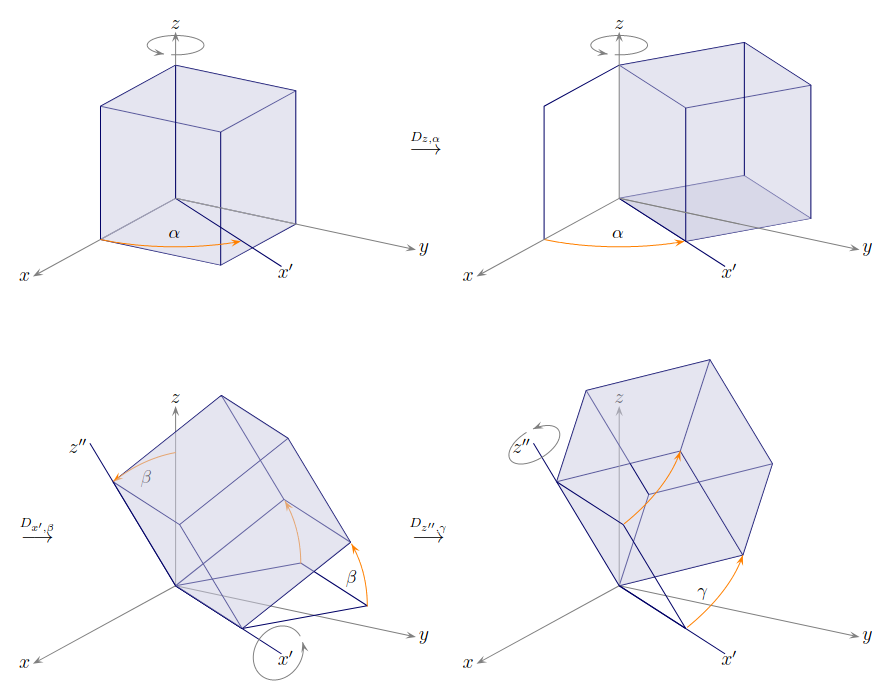
\includegraphics[scale=0.5]{../images/0026 Eulerwinkel.png}{\\Intrinsische Rotationsmodellierung in Eulerwinkel bei z-x'-z'' Konvention \ref{bild:1}}
\end{center}
Ist die Drehlage eines Objekts durch Eulerwinkel definiert können Drehmatrizen herangezogen werden als Operatoren welche Drehlageänderungen beschreiben. Das Drehmatrizentripel welches mit Eulerwinkeln funktionieren hat 3x3 Matrizen als Elemente \ref{link:Eulerwinkel}. Die Rotationsmatrizen können achsenspezifisch wie folgt definiert werden
\begin{align}
	D_{x,\varphi} &= \begin{pmatrix}
		1 & 0 & 0\\
		0 & \cos{\varphi} & -\sin{\varphi}\\
		0 & \sin{\varphi} & \cos{\varphi}
	\end{pmatrix}\\
	D_{y,\varphi} &= \begin{pmatrix}
		\cos{\varphi} & 0 & \sin{\varphi}\\
		0 & 1 & 0\\
		-\sin{\varphi} & 0 & \cos{\varphi} 
	\end{pmatrix}\\
	D_{z,\varphi} &= \begin{pmatrix}
		\cos{\varphi} & -\sin{\varphi} & 0\\
		\sin{\varphi} & \cos{\varphi} & 0\\
		0 & 0 & 1
	\end{pmatrix}.
\end{align}
Rotationsmatrizen lassen sich zu einer Eulerrotation $D_{Euler}$ verketten
\begin{align}
	D_{Euler} &= D_{z, \alpha}\circ D_{x', \beta}\circ D_{z'', \gamma}. 
\end{align}
Mit der Matrizenmultiplikation als Operator berechnet sich $D_{Euler}$ zu folgender 3x3 Rotationsmatrizen
\begin{align}
	D_{Euler} &= \begin{pmatrix}
		\cos{\alpha}\cos{\gamma} - \sin{\alpha}\cos{\beta}\sin{\gamma} & -\cos{\alpha}\sin{\gamma} - \sin{\alpha}\cos{\beta}\cos{\gamma} & \sin{\alpha}\sin{\beta}\\
		\sin{\alpha}\cos{\gamma} + \cos{\alpha}\cos{\beta}\sin{\gamma} & -\sin{\alpha}\sin{\gamma} + \cos{\alpha}\cos{\beta}\cos{\gamma} & -\cos{\alpha}\sin{\beta}\\
		\sin{\beta}\sin{\gamma} & \sin{\beta}\cos{\gamma} & \cos{\beta}
	\end{pmatrix}.
\end{align}
Die Determinante und die Eigenwerte von Rotationsmatrizen sind +1. Wird eine Verkettung vieler Rotationsmatrizen numerische berechnet, kommt es aufgrund von Rundungsfehler zu einem abdriften der Eigenwerte. Um dem entgegenzuwirken werden die Drehlage-Vektoren in der Praxis periodisch normiert.

\subsubsection{Kardanwinkel}
Kardanwinkel welche auch als Tait-Bryan-Winkel genannt werden, gehören zur Klasse der Eulerwinkel sind aber keine Eulerwinkel im klassischen Sinne \ref{link:Eulerwinkel}. Im Gegensatz zu den klassischen Eulerwinkeln wird um jede Achse gedreht und nicht bei der dritten Drehung nochmal um die erste Achse.
\begin{center}
	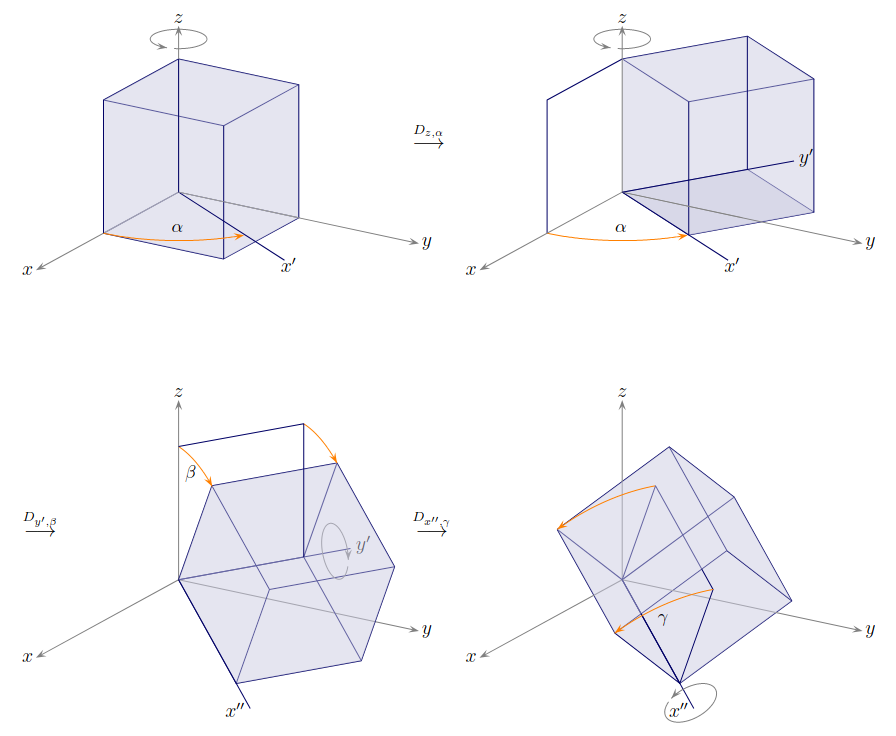
\includegraphics[scale=0.5]{../images/0028 Kardanwinkel.png}{\\Intrinsische Rotationsmodellierung in Kardanwinkeln bei z-y-x Konvention \ref{bild:1}}
\end{center}
Es existieren auch Sechs Permutationen von Kardanwinkeln. 
\begin{align}
	D_x-D_{y'}-D_{z''}\\
	D_y-D_{x'}-D_{z''}\\
	D_x-D_{z'}-D_{y''}\\
	D_z-D_{x'}-D_{y''}\\
	D_z-D_{y'}-D_{x''}\\
	D_y-D_{z'}-D_{x''}
\end{align}
Die Drehlagerepräsentation des Quadcopters erfolgt in der Konvention $D_z-D_{y'}-D_{x''}$ also mit Kardanwinkeln, sofern nicht Quaternion zur Drehlagerepräsentation verwendet wurden.

\subsubsection{Flugsystemlage}
Flugzeuge, Helikopter, Quadcopter und Raketen sind Objekte welche beliebt im dreidimensionalen Raum orientiert sein können. Bei den genannten Objekten sind bestimmte Drehlagen zu gewissen Zeiten unerwünscht. Will man die Objekte in eine Solldrehlage bringen muss man ihre Drehlage quantifizieren. Dazu eignen sich Kardanwinkel. Besser geeignet sind Kardanwinkel mit modellspezifischer Achsenbezeichnung. Fachleute sprechen aus diesem Grund von Rollwinkel $\phi$, Nickwinkel $\theta$ und Gierwinkel $\psi$ \ref{link:SimCon}.
Die Fluglagenwinkel können zu einem Vektor
\begin{align}
	\varphi &= \begin{pmatrix}
		\phi\\
		\theta\\
		\psi
	\end{pmatrix}
	\Leftrightarrow 
	\begin{pmatrix}
		D_{x''}\\
		D_{y'}\\
		D_{z}
	\end{pmatrix}.
\end{align}
zusammengefasst werden. Zu erkennen ist zudem die gewählte Äquivalentbeziehung zwischen Kardanwinkeln und Fluglagenwinkeln.
\begin{center}
	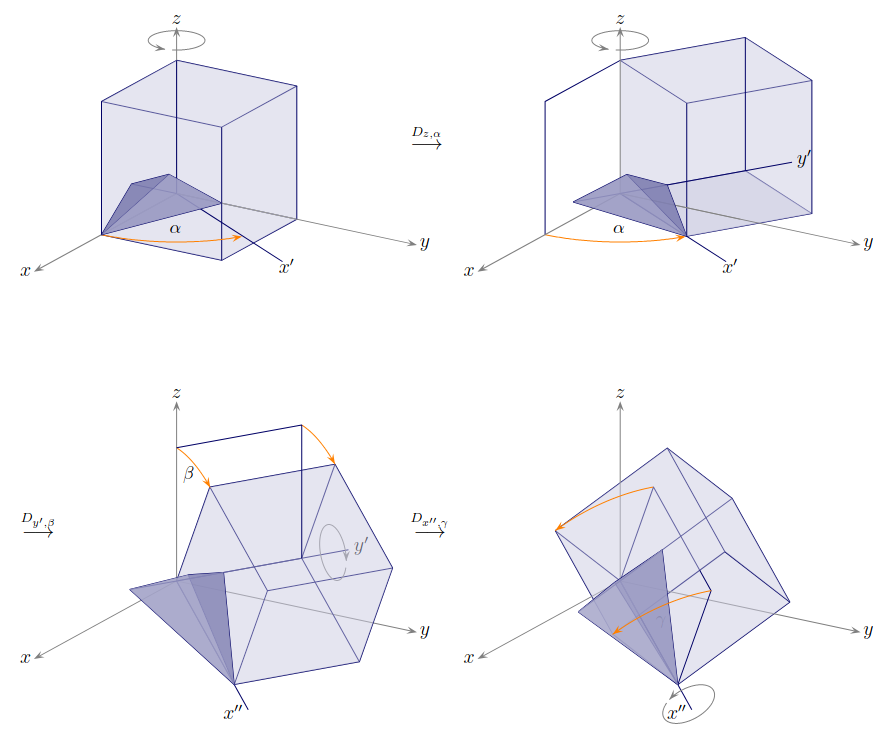
\includegraphics[scale=0.5]{../images/0029 Roll-Pitch-Yaw.png}{\\Zunächst wird gegiert, dann genickt und dann gerollt. Die Winkelvorzeichen wurden für alle Implementierungen übernommen. \ref{bild:1}}
\end{center}

\subsubsection{Gimbel Lock}
Eulerwinkel punkten in Sachen anschaulich haben aber ein signifikantes strukturelles Problem.
Wird beispielsweise zunächst mit einem beliebigen Winkel $\alpha$ um die z-Achse gedreht, dann mit dem Winkel $\frac{\pi}{2}$ um die $y'$-Achse entspricht die dritte Rotationsachse der Ersten \ref{link:Eulerwinkel}. Immer wenn das der Fall ist, geht ein Freiheitsgrad verloren und der Zustand Gimbel-Lock tritt ein. Die Bezeichnung ist entstanden, weil kardanischen Lagerungen (eng. Gimbel) welche bei Messinstrumenten zum Einsatz kommen in den unerwünschten Zustand gebracht werden können.
\begin{center}
	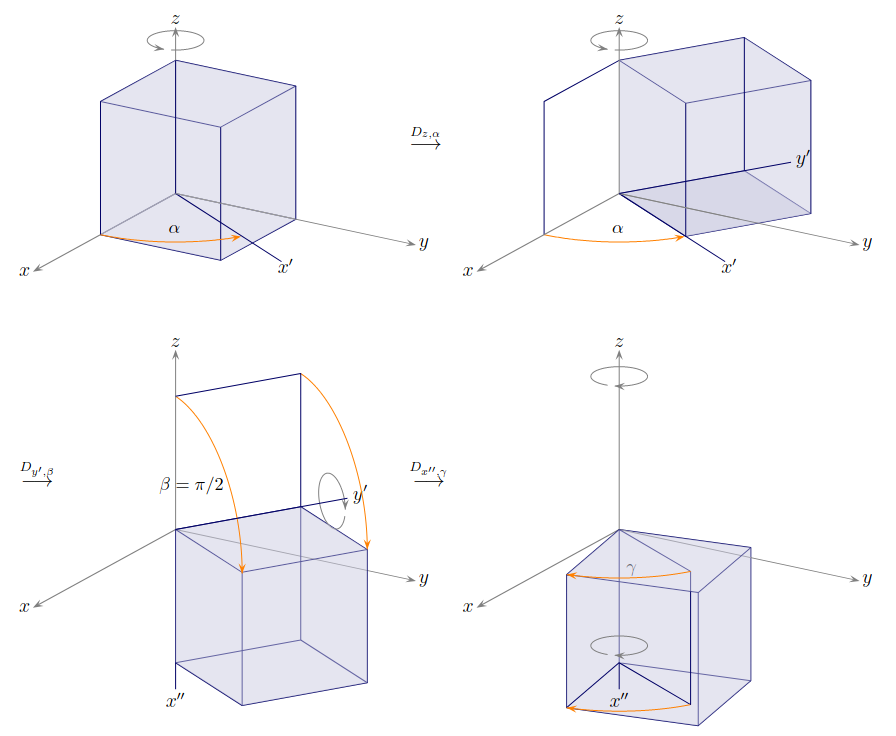
\includegraphics[scale=0.5]{../images/0027 Gimbel Lock.png}{\\Gimbel Lock auf der z-Achse nachdem zweimal um die z-Achse gedreht wird. \ref{bild:1}}
\end{center}


\subsubsection{Quaternionen}
Eulerwinkel sind anschaulich aber nicht besonders handlich für die mathematische Modellierung von Drehlagen und Rotationsprozessen. Grund dafür ist unter anderem Gimbel Lock.\\
Quaternionen sind vierdimensionale Zahlen mit speziellen Eigenschaften die insbesondere aufgrund von ihren, die Zustandseindeutigkeit und Laufzeit betreffenden Vorteilen, im Bereich der Drehlagen und Rotationsprozesse eingesetzt werden. Eine Quaternion
\begin{align}
	q &= q_w + iq_x + jq_y + kq_z,\ q_w, q_x, q_y, q_z \in R
\end{align}
wird in kartesischer Form notiert mit drei imaginären Einheiten $i$, $j$ und $k$ welche allesamt Lösungen für negative Einheitswurzeln sind
\begin{align}
	i &= j = k = \sqrt{-1}.
\end{align}
Die Norm einer Quaternion $|q|$ entspricht dem euklidischen Abstand berechnet auf allen Elementen
\begin{align*}
	|q| &= \left (q_w^2 + q_x^2 + q_y ^ 2 + q_z ^ 2\right )^{\frac{1}{2}}.
\end{align*}
Oft ist es notwendig eine Quaternion zu normieren da die Rotationsmodellierung nur mit Einheitsquaternionen funktioniert.
\begin{align}
	\frac{q}{|q|} &= \frac{q_w}{|q|} + i\frac{q_x}{|q|} + j\frac{q_y}{|q|} + k\frac{q_z}{|q|}
\end{align}
Zu jeder Quaternion existiert mit
\begin{align}
	q^{-1} &= \frac{1}{|q|}(q_w - iq_x - jq_y - kq_z)
\end{align}
eine Inverse für die gilt
\begin{align}
	qq^{-1} &= q^{-1}q = 1.
\end{align}
Geht man von einer Rotation in Form von einem Winkel
\begin{align}
	\theta &\in [0, 2\pi]
\end{align}
und einem Eulervektor
\begin{align}
	v &= \begin{pmatrix}
		v_x\\
		v_y\\
		v_z
	\end{pmatrix}
	\in R^3
\end{align} 
als einen Vektor mit Elementen eines dreidimensionalen Vektorraumes aus und will diesen als Quaternion ausdrücken kann dies über trigonometrische Funktionen passieren
\begin{align}
	\begin{pmatrix}
		q_w\\
		q_x\\
		q_y\\
		q_z
	\end{pmatrix}
	&= \begin{pmatrix}
		\cos\left (\frac{\theta}{2}\right )\\
		v_x \sin \left (\frac{\theta}{2}\right )\\
		v_y \sin \left (\frac{\theta}{2}\right )\\
		v_z \sin \left (\frac{\theta}{2}\right )
	\end{pmatrix}.
\end{align}
Soll ein Vektor oder Punkt $p = (p_x, p_y, p_z) \in R^3$ im dreidimensionalen Raum rotiert werden transformiert man zunächst den Vektor in eine Quaternion, indem der Realteil zu null gesetzt wird und die drei Imaginärteile aufsteigend mit den Elementen des Vektors gleichsetzt werden
\begin{align}
	q_p &= \begin{pmatrix}
		0\\
		p_x\\
		p_y\\
		p_z
	\end{pmatrix}.
\end{align}
Die Rotation wird nun berechnet, indem zunächst die Rotationsquaternion auf $q_p$ multipliziert wird und dann die Inverse der Rotationsquaternion multipliziert wird
\begin{align}
	q_p' &= qq_pq^{-1}.
\end{align}
Kardanwinkel lassen sich zu einer Quaternion umrechnen
\begin{align*}
	\begin{pmatrix}
		q_w\\
		q_x\\
		q_y\\
		q_z
	\end{pmatrix}
	&=
	\frac{1}{|q|}
	\begin{pmatrix}
		\cos(0.5\psi)\cos(0.5\theta)\cos(0.5\phi) + \sin(0.5\psi)\sin(0.5\theta)\sin(0.5\phi)\\
		\cos(0.5\psi)\cos(0.5\theta)\sin(0.5\phi) - \sin(0.5\psi)\sin(0.5\theta)\cos(0.5\phi)\\
		\cos(0.5\psi)\sin(0.5\theta)\cos(0.5\phi) + \sin(0.5\psi)\cos(0.5\theta)\cos(0.5\phi)\\
		\sin(0.5\psi)\cos(0.5\theta)\cos(0.5\phi) - \cos(0.5\psi)\sin(0.5\theta)\cos(0.5\phi)
	\end{pmatrix}
\end{align*}
und die Umkehrabbildung ist, ebenfalls nach \ref{link:Quaternion}, folgende
\begin{align}
	\begin{pmatrix}
		\psi\\
		\theta\\
		\phi
	\end{pmatrix}
	&= 
	\begin{pmatrix}
		\text{arctan}\left (\frac{2(q_xq_y + q_0q_z)}{q_w ^ 2 + q_x ^ 2 - q_y ^ 2 - q_z ^ 2}\right )\\
		\text{arcsin}\left (-2(q_yq_z + q_wq_x)\right )\\
		\text{arctan}\left (\frac{2(q_yq_z+q_wq_x)}{q_w ^ 2 - q_x ^ 2 - q_y ^ 2 + q_z ^ 2}\right )
	\end{pmatrix}.
\end{align}


\section{Systemtheoretische Vorbetrachtungen}
\subsection{Modellierung und Quadcoptersystem}
\subsubsection{Allgemeine Anforderungen an ein Dynamikmodell}
Unter einem Modell versteht man in der Philosophie eine Abbildung oder Repräsentation eines Objektes, eines Verhaltens oder eines Systems, das man verstehen möchte \ref{link:Modelle}.\\
Im Falle des Quadcopters galt es ein Dynamikmodell zu finden welches dessen Verhalten ausreichend gut abbildet um alle gesetzten Ziele zu erreichen. Aus dem primär, gesetzten Ziel, der Entwicklung eines flugfähigen Quadcopters, lassen sich Anforderungen ableiten.
Zum einen sollen die Vorhersagen des Modells über den tatsächlichen Zustand des Quadcopters nur bis auf einen maximalen Fehler abweichen von demjenigen Zustand, den man beobachten würde bei einem Quadcopter mit gleichen Input- und Systemparametern. Weicht auch nur ein vorhergesagter Wert weiter von seinem Soll ab als gewünscht ist das Modell unbrauchbar. Bei jedem Modell ist zu erwarten, dass die Vorhersagen in einer dynamischen Umwelt degradieren. Aus diesem Grund sollte die Qualität eines Modells auch abhängig von der Zeit betrachtet werden. Da für die Entwicklung eines Fluglagereglers nur Zustände innerhalb eines Flugintervalls vorhergesagt werden müssen, wurde von dem Modell nur erwartet, dass es über den Zeitraum von circa 5 Minuten vorhersagen innerhalb der Fehlerschranken liefert.\\
Wird ein Modell nicht Grund auf neu entwickelt, sondern aus einer Quelle herangezogen gilt es zu Validieren, dass das Modell den Anforderungen entspricht.\\
Das Flugdynamikmodell sowie die Implementierung eines Quadcopterreglerns wurden aus einem öffentlichen Repository bezogen und angepasst.
\begin{align}
	\label{simcon:simcon}\text{https://github.com/bobzwik/Quadcopter\_SimCon}
\end{align}
Da die Praktikabilität bei dieser Arbeit im Vordergrund steht wurde das Modell nach minimalen Plausibilitätstest für gut befunden und übernommen. Unter anderen Umständen ist es sinnvoll umfangreichere Tests an unbekannten Modellen oder Black-Box-Software durchzuführen.
Diese Tests könnten Mängel der Vorhersagegenauigkeit des Modells, invalide gewählte Inputparameter oder numerische Stabilitäts- und Konvergenzprobleme mit höherer Wahrscheinlichkeit zu Tage treffen lassen. Insgesammt stand der Nutzen für den Prototypen in keinem Verhältnis zu den Kosten sodass sich fokusiert wurde auf die korrekte Implementierung aller Schnittstellen. 
\subsubsection{Teilsysteme des Quadcopters}
Ein technisches System kann zur Veranschaulichung nahezu beliebig oft unterteilt werden. Naheliegend ist beispielsweise Hardware- und Softwarekomponenten zu trennen. In dieser Arbeit wurde ein anderer Ansatz verwendet. Geclustert wurden Teilsysteme nach ihren primär abgeleiteten Flussgrößen. Primärziel eines Motors ist beispielsweise einen Impulsfluss zu generieren und abzugeben. Aus diesem Grund wird er zum Impulsflusssystem zugeordnet und nicht zum Energieflusssystem. Mikrocontroller nehmen in der Funktion als Quadcopterregler Informationssignale, Energiesignale und technisch gesehen auch Impulse auf, geben aber primär Informationssignale ab.\\
Entsprechend wurde eine Klassifizierung zentraler Teilsysteme erstellt. Die Simulationssoftware umfasst nicht die Reglersoftware auf einem Mikrocontroller sondern nur jene PC seitige. Die Parameter sind in \ref{simcon:simcon} bereits mit erwartbaren Werten initalisiert worden. Ziel bei der Entwicklung des Programms war die Simulationssoftware in ihrer Allgemeinheit zu bewahren sodass diese weitestgehend unabhängig vom realen Quadcopter entwickelt werden kann. Gewählt wurde diese Herangehensweise, da die Adaption des Modells auf den realen Quadcopter am Ende als weniger arbeitsaufwändig eingeschätzt wurde als kontinuirlich zu versuchen das Simulationsmodell mit der realen Quadcopter zu vergleichen. Gerade zu Beginn wäre letzteres Vorgehen unpraktikel da noch kein Quadcopterprototyp produzieren war.
\vspace*{0.5cm}
\begin{center}
	\begin{tabular}[h]{|l|l|l|l|}
		\hline 
		System & Komponenten & Modellparameter \\
		\hline 
		Gesamt & Quadcopter & Masse $m$ [kg]\\
		& & Trägheit Nord-Achse $I_{B,xx}$ $\left [\frac{kg}{m^2}\right ]$\\
		& & Trägheit Ost-Achse $I_{B,yy}$ $\left [\frac{kg}{m^2}\right ]$\\
		& & Trägheit Unten-Achse $I_{B,zz}$ $\left [\frac{kg}{m^2}\right ]$\\
		\hline
		Impulsfluss & BLDC-Motor und Propeller & Zeitkonstante $\tau$ [1]\\
		& & Dämpfung d [1]\\
		& & Motorbefehlsgewinn $k_p$ [1]\\
		& & Schubkoeffizient $k_{Th}$ $\left [\frac{Ns^2}{rad^2}\right ]$\\
		& & Drehmomentkoeffizient $k_{To}$ $\left [\frac{Nms^2}{rad^2}\right ]$\\
		& Rahmen & Länge $l$ [m]\\
		& & Breite $w$ [m]\\
		& & Motorüberhöhung $h_M$ [m]\\
		\hline
		Energiefluss & Akkumulator/Netzteil & Maximalstrom $u_{max}$ [V]\\
		& & Maximalstrom $i_{max}$ [A]\\
		& BLDC-Treiber & Solldrehzahl $u_{soll, gelb}$ [V]\\
		& & Versorgungsspannung $u_{soll, rot}$ [V]\\
		& & Referenzspannung $u_{soll, braun}$ [V]\\
		\hline
		Informationsfluss & Simulationssoftware & siehe \ref{software:Software}\\
		& Mikrocontroller & siehe \ref{Reglerimplementierung:Reglerimplementierung} \\
		\hline
	\end{tabular}
\end{center}
Weitere Parameter wie die Rahmenelastizität oder der BLDC-Motorstrom wurden nicht betrachtet und aus diesem Grund nicht aufgeführt. Auch nicht betrachtet wird verwendetes externes Equipment. Nennenswertes elektrisches Equipment welches verwendet wurde war ein Multimeter, ein Signalgenerator und ein Oszilloskop.\\
Das Gesamtsystem hat zehn Freiheitsgrade. Diese sind die Position und Drehlage in jeweils drei Dimension und die vier Rotordrehlagen.\\
Zentrale Komponente eines Quadcopters ist der Rahmen. In der Regel sind alle Komponenten mechanisch direkt mit diesem verbunden. Für die mechanische Dynamik des Systems ist insbesondere auch  die Position der Motoren relativ zum Schwerpunkt des Systems ausschlaggebened.
\subsubsection{Zustandsvektor und Quadcopterdynamikmodell}
Die volatilen Parameter des Systems lassen sich übersichtlich in Vektorform schreiben. Die Zahlen im Index entsprechen der Elementanzahl der jeweiligen Vektoren.
\begin{align}
	s_{21} &= 
	\begin{pmatrix}
		p_3\\
		q_4\\
		v_3\\
		\dot{\varphi} _3\\
		\omega_4\\
		\dot{\omega}_4
	\end{pmatrix}
	=
	\begin{pmatrix}
		\text{Position (NED) [m]}\\
		\text{Drehlage (Quadternionenform)}\\
		\text{Geschwindigkeit [m/s]}\\
		\text{Winkelgeschwindigkeit [rad/s]}\\
		\text{Drehlage der Rotoren [rad]}\\
		\text{Winkelgeschwindigkeit der Rotoren [rad/$s^2$]}
	\end{pmatrix}.
\end{align}
Das Flugdynamikmodell ist in \ref{simcon:simcon} mit der Methode von Kane aufgestellt worden. Im Gegensatz zu Newtons-Methode oder zur Lagrange-Methode lässt sich Kanes-Methode relativ einfach auf mehrdimensionale Probleme der klassischen Mechanik anwenden \ref{link:Kane}.\\
Das Modell berechnet den Zustandsänderungsvektor $\dot{s}$ welcher mit der Motorengesamtkraft als die Summe aller Motorkräfte
\begin{align}
	F_G &= \sum_{M=1}^4 F_M
\end{align}
und den rotationsdimensionsabhängigen Kraftdifferenzen 
\begin{align}
	F_{D} &= \sum_{M=1}^4 v_{D,M}F_M
\end{align}
berechnet wird zu
\begin{align}\label{zustandsvektor:zustandsvektor}
	\dot{s} &= 
	\begin{pmatrix}
		\dot{p}_x\\
		\dot{p}_y\\
		\dot{p}_z\\
		\dot{q}_w\\
		\dot{q}_x\\
		\dot{q}_y\\
		\dot{q}_z\\
		\dot{v}_x\\
		\dot{v}_y\\
		\dot{v}_z\\
		\ddot{\phi}\\
		\ddot{\theta}\\
		\ddot{\psi}
	\end{pmatrix} = 
	\begin{pmatrix}
		\dot{p}_x\\
		\dot{p}_y\\
		\dot{p}_z\\
		-0.5\dot{\phi} q_x - 0.5\dot{\theta} q_y - 0.5\dot{\psi} q_z\\
		+0.5\dot{\phi} q_w - 0.5\dot{\theta} q_z + 0.5\dot{\psi} q_y\\
		+0.5\dot{\phi} q_z + 0.5\dot{\theta} q_w - 0.5\dot{\psi} q_x\\
		-0.5\dot{\phi} q_y + 0.5\dot{\theta} q_x + 0.5\dot{\psi} q_w\\
		-2(q_wq_y + q_xq_z) F_G \frac{1}{m}\\
		+2(q_wq_x - q_yq_z) F_G \frac{1}{m}\\
		(-(q_w^2-q_x^2-q_y^2+q_z^2) F_G + mg) \frac{1}{m}\\
		((I_{B,yy} - I_{B,zz}) \theta \psi + F_{\phi} w) \frac{1}{I_{B,xx}}\\
		((I_{B,zz} - I_{B,xx}) \phi \psi + F_{\theta} l) \frac{1}{I_{B,yy}}\\
		((I_{B,xx} - I_{B,yy}) \phi \theta + F_{\psi})\frac{1}{I_{B,zz}}
	\end{pmatrix}.
\end{align}
Die Vorzeichenvektoren für die Roll-, Nick- und Gierachsen sind
\begin{align}
	v_{\phi} &= \begin{pmatrix}
		v_{\phi, M1}\\
		v_{\phi, M2}\\
		v_{\phi, M3}\\
		v_{\phi, M4}
	\end{pmatrix} =
	\begin{pmatrix}
		1\\
		-1\\
		-1\\
		1
	\end{pmatrix},\
	v_{\theta} =
	\begin{pmatrix}
		1\\
		1\\
		-1\\
		-1
	\end{pmatrix},\
	v_{\psi} =
	\begin{pmatrix}
		-1\\
		1\\
		-1\\
		1
	\end{pmatrix}.
\end{align}
Die Rotordrehlage und -geschwindigkeit jedes Motors welche auch Element des Zustandsvektors sind, können mithilfe von einer Differenzialgleichung
\begin{align}
	\ddot{\omega}_{M1} &= \frac{-2d}{\tau}\dot{\omega}_{M1} - \frac{1}{\tau^2}\omega_{M1} + \frac{k_p}{\tau^2}\Omega_{M1}\\
	\ddot{\omega}_{M2} &= \frac{-2d}{\tau}\dot{\omega}_{M2} - \frac{1}{\tau^2}\omega_{M2} + \frac{k_p}{\tau^2}\Omega_{M2}\\
	\ddot{\omega}_{M3} &= \frac{-2d}{\tau}\dot{\omega}_{M3} - \frac{1}{\tau^2}\omega_{M3} + \frac{k_p}{\tau^2}\Omega_{M3}\\
	\ddot{\omega}_{M4} &= \frac{-2d}{\tau}\dot{\omega}_{M4} - \frac{1}{\tau^2}\omega_{M4} + \frac{k_p}{\tau^2}\Omega_{M4}.
\end{align}
für jeden Motor berechnet werden.
Dabei ist $\tau$ eine Zeitkonstante, $d$ die Dämpfung und $k_p$ der Gewinn der Motorbefehle $\Omega_{M}$.
Die Drehzahlbeschleunigung ist abhängig von der Drehrate und der Drehzahl sowie dem Motorbefehlen $\omega_{Mx}$. Aus einer Rotordrehzahl kann mit dem Schubkoeffizient auf den Schub
\begin{align}
	\text{Schub} &= k_{Th}\cdot \omega^2
\end{align} und mit dem Drehmomentkoeffizient auf das Drehmoment
\begin{align}
	\text{Drehmoment} &= k_{To}\cdot \omega^2
\end{align}
geschlossen werden.\\
Auf eine ausführliche Herleitung und Beschreibung des Modells wird an dieser Stelle verzichtet da das Modell als Systemkomponente betrachtet wurde und nicht als Kernkomponente.\\
Nicht verzichtet werden soll auf den Hinweis, dass ein Quadcopter ein sehr instabiles System ist. Selbst bei gleich verteilten Motorbefehlen mit dem Erwartungswert gleich den Schwebebefehlen fängt das System stark an zu rotieren.
\begin{center}
	\includegraphics[scale=0.3]{../images/0047 Eulerwinkel Zufällige Aktionen.png
	}{\\Drehageentwicklung bei zufälligen gleichverteilten Rotorbefehlen nach 5s. Je stärker der Erwartungswert absolut von den Schwebebefehlen abweicht und je größer die Varianz der Wahrscheinlichkeitsverteilung desto instabiler wird System. Im Bild kann sich der Quadcopter aufgrund seiner Trägheit für circa 5e-1s stabil halten das ist nicht der Regelfall.}
\end{center}



\subsection{Regelungstechnik}

\subsubsection{Regelungsproblem}
Die Regelungstechnik hilft, wenn einer Solltrajektorie wegen Modellgenauigkeiten oder\\ Störgrößen nicht gefolgt werden kann. Durch Vergleich der Solltrajektorie mit der tatsächlich Trajektorie und Rückkopplung über einen Regler werden die Eingangsgrößen des zu regelnden Systems angepasst und die Trajektorie korrigiert \ref{link:Regelungstechnik1}. Man ist bestrebt einen Regler zu finden welcher das Verhältnis aus Reglergüte und Implementierungskosten maximiert.

\subsubsection{Fehler}
Ein Fehler ist ein Maß für ungewollte Abweichung zwischen zwei Objekten gleichen Datentyps, beispielsweise Punkten auf zwei Trajektorien. Fehler können verglichen werden. Kein Fehler ist gleichbedeutend mit den äquivalenten Objekten. Der minimalste Fehler ist keiner. Fehler lassen sich theoretisch auf verschiedene Weisen berechnen, die Methode mit den geringsten Rechenkosten ist 
\begin{align}
	e(t) &= s_{Soll}(t) - s_{Ist}(t)
\end{align}
die Subtraktion von Sollwert $s_{Soll}$ und Istwert $s_{Ist}$ \ref{link:Regelungstechnik1}.

\subsubsection{Regler}
Ein Regler ist ein Algorithmus welcher einen oder mehrere Fehler sampelt und basierend auf den Fehlern regelbasiert Signale generiert mit dem Ziel keinen Fehler zu produzieren. Ein Regler ist eingebettet in ein rückgekoppeltes dynamisches System \ref{link:Regelungstechnik1}.

\subsubsection{\label{pid:pid}PID-Regler}
PID-Regler sind eine Klasse von Reglern mit geringen Implementierungskosten.
Die Elemente der Klasse, auch Glieder genannt, beispielsweise P-Glied, lassen sich addititiv kombinieren mit anderen Elementen wie den I-Glied oder dem D-Glied.
Ein PID-Regler berechnet eine Stellgröße $u$ aus einem Fehler $e$ nach der Vorschrift
\label{pidregler}
\begin{align}
	u(t) = K_Pe(t) + K_I\int_0^t e(\tau)d\tau + K_D\frac{de}{dt}.
\end{align}
Durch die Optimierung der Parameter $K_P$, $K_I$ und $K_D$ kann der Regler auf ein System abgestimmt werden \ref{link:Regelungstechnik1}. Ohne ein I-Glied wäre der PID-Regler nicht in der Lage stationäre Regelabweichung auf Null zu regeln. D-Glieder sind deutlich schneller als P-Glieder und werden dann eingesetzt wenn die Anforderungen welche von der Systemdynamik ausgehen hoch sind. Quadcopter stellen derartige Anforderungen an einen Regler. Bei D-Gliedern ist darauf zu achten, dass die gezeigte Form zu Impulsspitzen bei der Stellgröße führt. In Praxis kann das Verhalten minimiert werden indem statt dem Fehler nur der Istzustand differenziert wird oder ein Tiefpass zugeschaltet wird \ref{link:Regelungstechnik1}. 

\subsubsection{\label{Quadcopterregelungsproblem}Quadcopterregelungsproblem}
Ein intuitiver Ansatz für das Design eines Quadcopterlage- und -geschwindigkeitsreglers könnte sein alle Sollwertachsen, also die Roll-, Nick- und Gierachse sowie die drei Geschwindigkeiten auf der Nord-, Ost- und Unten-Achse jeweils mit einem PI- oder besser einem PID-Regler zu versehen. Doch bevor sich auf die Implementierung eines solchen Reglers gestützt werden kann stellt man hoffentlich fest, dass aus der Beschreibung des Reglers in keiner Weise hervorgeht wie die Stellgrößen von PID-Regler auf die Motoren wirken. Für die Drehlage-PID-Regler wäre denkbar, dass beispielsweise eine Nickbewegung zu einer Erhöhung der Drehzahl der BLDC-Motoren auf der Vorderseite führen muss. Äquivalent könnte für die anderen Drehachsen vorgegangen werden. Bis man feststellt, dass die Gierachse orthogonal steht zu den Motorachsen. Auch nicht weiter tragisch, denn mithilfe von differenzieller Motordrehzahlen kann der Quadcopter um die Gierachse gedreht werden. Dazu muss bei einem positiven Gierfehler die Summe der Rotordrehmomente negativ sein. Durch Addition der Stellwerte aller Regler könnten die Motorbefehle berechnet werden. Spätestens beim Versuch den Geschwindigkeitsregler auf ähnliche Weise beizumischen wird aber deutlich, Quadcopter sind in hohem Maße nichtlinear bedingt durch die systemeigene Geometrie. In \ref{simcon:simcon} hat man sich für einen spezielleren Regler entschieden schlichtweg, weil der intuitive Standard-PID-Regler an seine Grenzen kommt. Nichtlineare Systeme können oft gar nicht mit Methoden aus der linearen Regelungstechnik stabilisiert werden stattdessen müssen neue, oftmals gänzlich andere, Klassen von Verfahren und Algorithmen zur Regelung betrachtet werden. Stichworte aus dem Bereich der nichtlinearen Regelungstechnik sind, Linearisierung, Modellprädiktive Regelung \ref{link:MPC}, $H_{\infty}$-Regelung und nichtlineare Regelung mit tiefen Netzwerken \ref{link:Regelungstechnik2}. Durch Linearisierung kann ein nichtlineares Zustandsraummodell in ein lineares transformiert werden. Modellprädiktive Regelung und gerade $H_{\infty}$-Regler sind in der Luft- und Raumfahrtbranche häufig angewendet Verfahren mit hoher Robustheit. Wobei $H_{\infty}$-Regler für lineare Modelle entwickelt wurden aber adaptiert werden können auf nichtlineare. Die tiefen Netzwerke müssen an der Stelle kurz hinten anstehen werden in dieser Arbeit noch eine hohe Bedeutung zugemessen bekommen. Die anderen Verfahren wurden nicht weiter betrachtet, nicht weil sie ungeeignet oder uninteressant sind, sondern weil sie den Weg mit dem höheren Lern- und Implementierungswiderstand darstellten. Und auch da in \ref{simcon:simcon} bereits ein anderer erfolgversprechender Regler vorgefunden wurde, inspiriert ist dieser von \ref{link:ETH}. Das Kontrollgesetz zur Drehlageregelung ist dabei mit $\tau$ einer Zeitkonstante für eine Differenzialgleichung erster Ordnung, $q$ einer Fehlereinheitsquaternion welche die Abweichung von der Sollfluglage beschreibt und $\Omega$ den Solldrehgeschwindigkeiten.
\begin{align}
	\Omega(q) &= \frac{2}{\tau}\text{sgn}(q_{w})q_{x:z}.
\end{align}
Die Autoren von \ref{link:ETH} konnten zeigen, dass das Kontrollgesetz in relevanten Bereichen asymptotisch stabil und eindeutig ist. Ein Problem bleibt allerdings, so die Autoren, dass die Robustheit gegenüber auch leistungsschwachem Messrauschen gering ist. Das Problem scheint rein theoretischer Natur zu sein und auf Digitalreglern in der Praxis nicht relevant zu sein \ref{link:ETH}. Für eine detailierten Beschreibung der Sollquaternionberechnung wird auf die Quelle und das Kapitel \ref{Reglerimplementierung:Reglerimplementierung} hingewiesen. Dort wird des weitern erleutert welche PID-Parameter an welchen Stellen wirken.
\begin{center}
	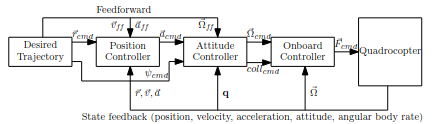
\includegraphics[scale=0.78]{../images/0001 Quadcopterregler.png}{\\Für den später verwendeten Regler wurden die Solltrajektorie zu einem Sollgeschwindigkeitsvektor vereinfacht und nur die Geschwindigkeit geregelt. Das Bild ist entnommen aus der ursprünglichen Veröffentlichung \ref{link:ETH}.}
\end{center}


\subsection{Tiefes verstärkendes Lernen}

\subsubsection{Lernproblem}
Lernen ist ein Prozess welcher darauf abzielt Zustände zu finden von welchen aus heraus der zu überblickende Aktionsraum optimaler ist als in allen vorangegangen Zuständen. 
Optimaler bedeutet der Wert des Zustandes ist maximal innerhalb der Menge aller besuchten Zustände.\\
Ein Lernproblem ist ein Problem bei welchem es im Kern darum geht Systemparameter zu finden welche zu optimalem Lernverhalten führen. 
Das Lernproblem ist eng verknüpft mit dem Teilbereich Optimierung der Elektrotechnik. 

\subsubsection{Analogien zur Regelungstechnik}
Lernende Systeme haben dasselbe Ziel wie klassische Regler sind aber in der Lage Fehler in einer Umwelt zu finden, auf die Sie nicht explizit ausgelegt wurden. Oft ist es erforderlich, dass ein Regler lernt, beispielsweise wenn sich die Reglerumwelt dynamisch ändert.\\
Tiefes verstärkendes Lernen (eng. Deep reinforcement learning) ist ein Lernparadigma das tiefe Netzwerk mit Fehlrückführungsalgorithmus und belohnungsbasierten Lernen fusioniert. Tiefe Netzwerke werden in der Regelungstechnik schon eine Weile als Regler verwendet \ref{link:Regelungstechnik2}. Eine jüngere Entwicklung ist der Einsatz des tiefen verstärkenden Lernen.
In der Regelungstechnik determinieren externe Sollwerte das Verhalten, also Werte, die aus einer Umwelt kommen, welche nicht lokal geregelt werden sollen. Im verstärkenden Lernen gibt es keine Sollwerte im Sinne der Regelungstechnik, sondern Belohnungen, welche eine Funktion der Umwelt sind, die geregelt werden soll. Will man beispielsweise die Rotationsgeschwindigkeit der Erde regeln kann man ein verstärkender Regler mit dem inversen Abstand zwischen Soll- und Istgeschwindigkeit belohnen. Auch möglich wäre die Belohnung mit der Zufriedenheit der Erdbewohner skalieren zu lassen vorausgesetzt man kann diese messen. Das Beispiel soll verdeutlichen, dass der Belohnungsbegriff einen direkteren Bezug zur Optimierung hat und mehrdeutiger ist als der Fehlerbegriff aus der klassichen Regelungstechnik.
\begin{center}
	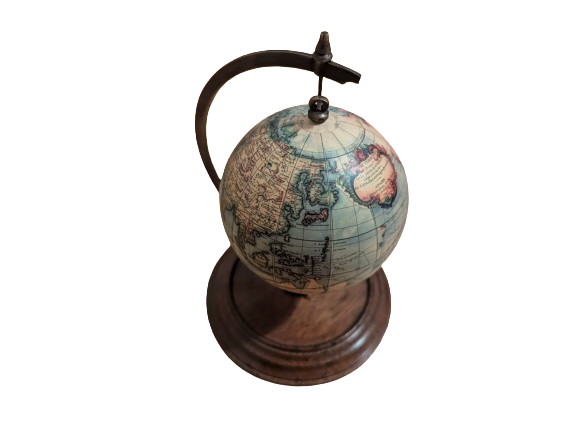
\includegraphics[scale=0.26]{../images/0046 Weltmodell ohne Hintergrund.png
	}{\\Modell der Erde und eindimensionalles Rotationsmodell zugleich}
\end{center}

\subsubsection{Vokabular des tiefen verstärkenden Lernens}
Tiefes verstärkendes Lernen ist ein breites Feld welches zahlreiche Lernalgorithmen umfasst. In dieser Arbeit wurde der Fokus auf modellfreie Policy-Gradient-Algorithmen, insbesondere Proximal-Policy-Optimization \ref{ppo} gelegt. Das Vokabular hat nicht den Anspruch alle Begriffe und Methoden einzuführen, sondern nur wenige die Policy-Gradient-Methoden zugrunde liegen.\\
Im verstärkenden Lernen werden Regler auch als Agenten bezeichnet. Dadurch wird unter anderem die Verbindung zur Robotik betont.\\
Der heilige Gral im verstärkenden Lernen ist das Lernen einer umweltspezifischen optimalen Strategie $\pi$ \ref{link:MaschinellesLernen}. Eine Strategie kann als Abbildung von Zuständen $s_t$ auf eine Wahrscheinlichkeitsverteilung über Aktionen $a_t$
\begin{align}
  a_t &= \pi(s_t)
\end{align}
in jedem Zeitschritt $t$ betrachtet werden \ref{link:MaschinellesLernen}. Vor dem Lernprozess ist eine Strategie zufällige initialisiert. Während dem Lernprozess ist das Ziel die Strategie so anzupassen, dass die optimale Aktion am stärksten gewichtet werden und das bei minimalem Rechenaufwand.\\
Agenten, diejenigen Entitäten deren Aktionen optimiert werden sollen, berechnen Verbesserungen ihrer Strategie im, modellfreien verstärkenden Lernen, allein basierend auf Umweltbeobachtungen und Belohnungssignalen $r_t$. Die Belohnungsfunktion
\begin{align}
  r(a_t) &= r_t
\end{align}
eine Methode der Umwelt bildet Aktionen auf Belohnungen ab. Die Summe aller zukünftigen Belohnungen ausgehend von aktuellem Zustand wird als Gewinn (eng. Gain) bezeichnet. 
\begin{align}
  G_t &= \sum_{k = 0}^{\infty}\gamma ^kr_{t+k+1}. 
\end{align}
Belohnungen kodieren, eine Anforderungen an das lernende System \ref{link:MaschinellesLernen}.
Die Zustandswertefunktion
\begin{align}
  V^\pi(s) &= E(G_t | s_t)
\end{align}
bewertet Zustände hinsichtlich des zukünftig in dem Zustand zu erwartenden Gewinn beim Handeln nach der Strategie $\pi$ \ref{link:MaschinellesLernen}.\\
Die Zustandswertefunktion kann herangezogen werden, um die Strategie zu optimieren \ref{link:MaschinellesLernen}.\\
Policy-Gradient-Methoden optimieren die Strategie auf Basis von Erfahrungssamples welche abgespeicherte Informationen aus einem Batch an Episoden sind. Eine Episode entspricht einem Prozess vom Start bis zum Ende. Für einen Agenten welcher einen Quadcopter regelt ist eine Episode beispielsweise ein Flug. Mit aktuellen Methoden des verstärkenden Lernens ist es nicht ansatzweise ausreichend marktreife Regler in einer Episode anzulernen. Weshalb der Lernprozess eines Agenten in einer Simulation passiert und oft mehrere Millionen Episoden lang läuft.

\subsubsection{Tiefe Netzwerke}
Biologisch inspirierte lernfähige Netze können konstruiert werden, indem Schichten $S$ aus Funktionen verkettet werden und die Funktionsparameter mit einem Algorithmus iterativ angepasst werden, sodass eine Verlustfunktion minimiert wird.
\begin{align}
  y &= S_1(S_2(...S_d(x)...)).
\end{align}
Sie sind in der Lage beliebige Funktionen zu approximieren \ref{link:MaschinellesLernen}. Also ihre Schätzung der oder besser Vorhersage über die Funktionswerte näher an den tatsächlichen Funktionswert zu bringen.
\subsubsection{Mehrschichtiges Perzeptronennetzwerk}
Bei einem Standardnetzwerk, dem Perzeptronennetzwerk, besteht eine Schicht $S$ aus Knoten welche die gewichteten Outputs der Knoten aus der davorliegenden Schicht summiert zu
\begin{align}
  v_j^{(S)} &= \sum_i w_{ij}^{(S)}x_i
\end{align}
und eine nichtlineare Aktivierungsfunktion $\sigma$
\begin{align}
  O_j^{(S)} &= \sigma \left (v_j^{(S)}\right )
\end{align}
auf die Summe anwendet. Die Aktivierungsfunktion ermöglicht dem Netzwerk das Lernen von wenn-dann-Beziehungen. Der Output eines Knotens wird an alle Knoten der nachfolgenden Schicht weitergeleitet.
\vspace*{0.5cm}
\begin{center}
  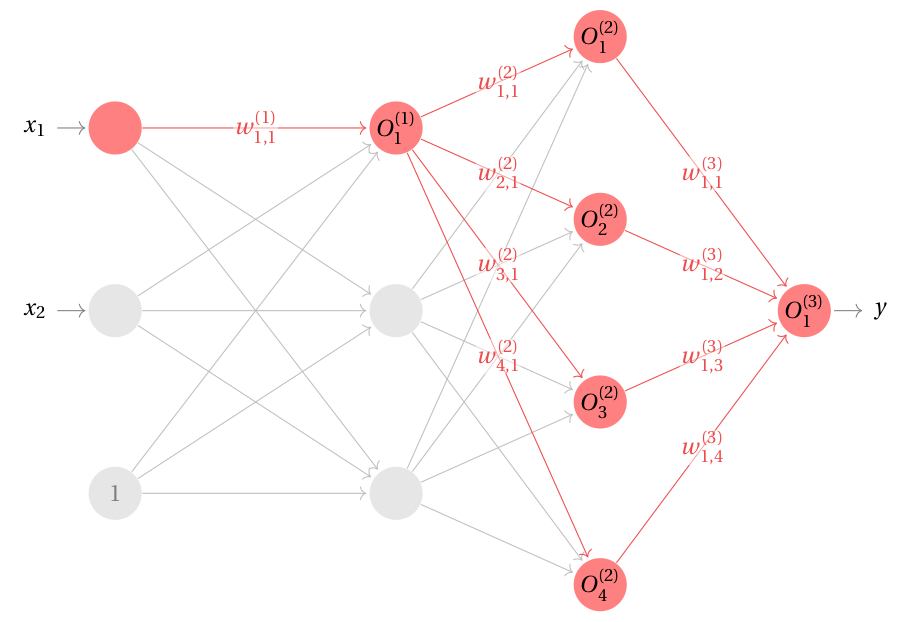
\includegraphics[
    width=0.7\textwidth, 
    keepaspectratio
  ]{../images/0032 multi-layer-perzeptron.png}{\\Ein voll verknüpftes Netzwerk in welchem alle Knoten rot sind die durch das Gewicht $w_{1,1}^{(S)}$ beeinflusst werden \ref{link:MaschinellesLernen}}
\end{center}

\subsubsection{Fehlerückführungsalgorithmus}
Die Gewichte eines Netzwerkes sollen so angepasst werden, dass der Fehler zwischen den Output des Netzwerkes $y_{Ist}$ und den Sollwerten $y_{Soll}$ minimal ist \ref{link:MaschinellesLernen}. Der Fehler $E$ wird mit einer Verlustfunktion (eng. Loss function) berechnet beispielsweise dem mittleren quadratischen Fehler
\begin{align}
  \min_{w_{ij}^{(S)}} E &= {
    \min_{w_{ij}^{(S)}}\frac{1}{2}\left (y_{\text{Soll}} - y_{Ist}\right )^2
  }.
\end{align}
Das entwickelte Optimierungsproblem, für die Gewichte $w_{ij}^{(S)}$, wird iterativ mit dem Gradientenabstiegsverfahren 
\begin{align}
  w_{ij,t+1}^{(S)} &= {
    w_{ij, t}^{(S)} - \mu \frac{\partial E}{\partial w_{ij, t}^{(S)}}
  }
\end{align}
gelöst bei einer Lernrate $\mu $ \ref{link:MaschinellesLernen}.\\
Die partielle Ableitung der Verluste als Funktion der Gewichte kann berechnet werden durch die Anwendung der Kettenregel
\begin{align}
  \frac{\partial E}{\partial w_{ij}^{(S)}} &= {
    \sum_j \left (y_{\text{Soll}} - y_{\text{Ist}}\right )\frac{\partial y}{\partial w_{ij}^{(S)}}
  }.
\end{align}
Der Output des Netzwerks $y_{Ist}$ entspricht dem Output der letzten Schicht des Netzwerks
\begin{align}
  \frac{\partial E}{\partial w_{ij}^{(S)}} &= \sum_j \left (y_{\text{Soll}} - y_{\text{Ist}}\right )\frac{\partial \sigma \left (v_j^{(S)}\right )}{\partial w_{ij}^{(S)}}.
\end{align}
Die Kettenregel wird erneut verwendet um die partielle Ableitung der Aktivierungsfunktion nach den Gewichten zu berechnen
\begin{align}
  \frac{\partial E}{\partial w_{ij}^{(S)}} &= \sum_j \left (y_{\text{Soll},j} - y_{\text{Ist}}\right )\sigma'\left (v_j^{(S)}\right )\frac{\partial v_j^{(S)}}{\partial w_{ij}^{(S)}}.
\end{align}
Die Inputgewichte werden proportional zum Fehler, der Aktivierung und dem Output des Netzwerks
\begin{align}
  \frac{\partial E}{\partial w_{ij}^{(S)}} &= \sum_j \left (y_{\text{Soll},j} - y_{Ist, j}\right )\sigma'\left (v_j^{(S)}\right )O_j
\end{align}
aktualisiert \ref{link:MaschinellesLernen}.

\subsection{\label{ppo}Proximal-Policy-Optimization}
Proximal-Policy-Optimization ist ein Policy-Gradient-Algorithmus aus dem Bereich des tiefen verstärkenden Lernens \ref{link:PPOSpinningUp}.\\
Kernelement von Proximal-Policy-Optimization sind zwei tiefe Netzwerke welche im Sinne einer Actor-Critic-Architektur zusammen fungieren. Die Idee dabei ist, dass Aktionen eines Strategienetzwerks kontinuierlich bewertet beziehungsweise kritisiert werden durch ein Netzwerk welches die Zustandswertefunktion approximieren. Das Strategienetzwerk nimmt die Rolle des Actors ein und das Zustandswertenetzwerk die des Critics.\\
Proximal-Policy-Optimization lernt nicht in jedem \textit{step} die Strategie, sondern nach einer oder mehreren Episoden \ref{link:PPOSpinningUp}. Diese Form des agieren auf der Umwelt mit der probabilistischen Strategie wird Rollout genannt. Um alle Aktionswahrscheinlichkeiten, Aktionen, Beobachtungen und Belohnungen, seit der letzten Lernphase, für die Optimierung einzubeziehen werden diese in Batches abgespeichert. Es gilt des weitern Verlustfunktionen zu berechnen um die Strategie- und Zustandswertenetzwerke zu optimieren. Aufseiten des Critics erfolgt dies auf Basis der gespeicherten Belohnungen, den sogenannten Unterwegsbelohnungen und der Vorhersage des aktuellen Zustandswertenetzwerks. Das Fehlermaß wird für die Verlustfunktion ist der Euklidische Abstand zwischen den tatsächlich erfahrenen Belohnungen $R$ und der aktuellen Annahme für $V^{\pi}$.\\
Für die Optimierung des Actors wird die Zustandswertefunktion als Kritik herangezogen. Durch Subtraktion der Zustandswerte einer Episode von den gesammelten Unterwegsbelohnungen wird auf Vorteile (eng. Advantages) A geschlossen. Diese quantifizieren die Güte der aktuellen Aktion im Vergleich zu allen möglichen Aktionen eines Zustandes.
Die Auftrittswahrscheinlichkeit der vom Actor gewählten Aktion zur letzten wird ratio genannt und bemisst die Divergenz zwischen neuer und alter Strategie. Das logarithmieren der Wahrscheinlichkeiten hilft beim Gradientenabstieg \ref{link:LogPPO}.
Eine zentrale Innovation von Proximal-Policy-Optimization gegenüber Vorgängern ist das der ratio auf den Wertebereich 0.8 und 1.2 eingekürzt wird. Durch diese Maßnahme wird sichergestellt, dass Aktionen nur gering voneinander abweichen. Der Lernprozess wird einheitlicher, konservativer und damit stabiler \ref{link:PPOSpinningUp}.
Durch die Multiplikation von Vorteilen A und ratio, siehe Bild, werden Hilfsfunktionen (eng. surrogate function) $S_1$ und $S_2$ berechnet. Durch Minimierung und Mittelwertbildung wird auf die Verluste für das Strategienetzwerk geschlossen.
\begin{center}
    \begin{tikzpicture}[font=\sffamily,every label/.append
    style={font=\small\sffamily,align=center}]

	\node[doc] at (1, 0) (Regler) {Rollout};

	\node[
		cylinder, 
		cylinder uses custom fill, 
		cylinder end fill=orange!25,
		cylinder body fill=orange!50,
		shape border rotate=90,
		text=white,
		aspect=0.4,
		minimum width=1cm,
		minimum height=1.4cm] at (4, -2) (BatchBelohnungen){Unterwegsbelohnung $R$};

	\node[cylinder, cylinder uses custom fill, cylinder end fill=violet!25,
	cylinder body fill=violet!25,shape border rotate=90,text=white,
	aspect=0.4,minimum width=1cm,minimum height=1.4cm] at (4, 0) (BatchLog){Log $log(p_{a,t-1})$};

	\node[cylinder, cylinder uses custom fill, cylinder end fill=red!25,
	cylinder body fill=red!50,shape border rotate=90,text=white,
	aspect=0.4,minimum width=1cm,minimum height=1.4cm] at (4, 2) (BatchAktionen){Aktionen $p_{a}$};

	\node[cylinder, cylinder uses custom fill, cylinder end fill=blue!25,
	cylinder body fill=blue!50,shape border rotate=90,text=white,
	aspect=0.4,minimum width=1cm,minimum height=1.4cm] at (4, 4) (BatchBeobachtungen){Beobachtungen $o$};

	\node[doc] at (7, 2) (Critic) {Actor};

	\node[doc] at (8, 4) (Evaluate) {Critic};

	\node[doc] at (7, 0) (Ratios) {$e^{x-y}$};

	\node[doc] at (7, -4) (Clamp) {Clip($0.8, 1.2$)};

	\node[circle, draw] (Advantage) at (8, -2) {-};

	\node[circle, draw] (Surr1) at (9, -2) {$\cdot$};

	\node[circle, draw] (Surr2) at (9, -3) {$\cdot$};

	\node[doc] at (12.25, -5) (MSE) {$\sqrt{R^2 - {V^{\pi}}^2}$};

	\node[doc] at (15.5, -2) (Backprop1) {Actor update\\$w_{ij} - \mu \frac{\partial L_{Actor}}{\partial w_{ij}^{(l)}}$};

	\node[doc] at (15.5, -5) (Backprop2) {Critic update\\$w_{ij} - \mu \frac{\partial L_{Critic}}{\partial w_{ij}^{(l)}}$};

	\node[doc] at (11, -2) (Mean) {$\overline{\min{S_1, S_2}}$};

	\draw[-latex] (Regler) |- (BatchBelohnungen);

	\draw[-latex] (Regler) |- (BatchAktionen);

	\draw[-latex] (Regler) |- (BatchBeobachtungen);

	\draw[-latex] (Regler) -- (BatchLog);

	\draw[-latex] (BatchBeobachtungen) -- (Evaluate);

	\draw[-latex] (BatchAktionen) -- (Critic);

	\draw[-latex] (BatchLog) -- (Ratios);

	\draw[-latex] (Evaluate) -- (Advantage) node[midway, above, font=\small\sffamily]{};

	\draw[-latex] (BatchBelohnungen) -- (Advantage);

	\draw[-latex] (Critic) -- (Ratios) node[midway, left, font=\small\sffamily]{$log(a)$};

	\draw[-latex] (Advantage) -- (Surr1) node[midway, below, font=\small\sffamily]{$A$};

	\draw[-latex] (Ratios) -| (Surr1) node[midway, right, font=\small\sffamily]{$ratio$};

	\draw[-latex] (Ratios) -- (Clamp);

	\draw[-latex] (Clamp) -| (Surr2) node[midway, right, font=\small\sffamily]{$clipped\ ratio$};

	\draw[-latex] (Advantage) |- (Surr2) node[midway, left, font=\small\sffamily]{$A$};

	\draw[-latex] (Surr1) -- (Mean) node[midway, below, font=\small\sffamily]{$S_1$};

	\draw[-latex] (Surr2) -| (Mean) node[midway, below, font=\small\sffamily]{$S_2$};

	\draw[-latex] (Mean) -- (Backprop1) node[midway, below, font=\small\sffamily]{$L_{Actor}$};

	\draw[-latex] (Evaluate) -| (MSE) node[midway, above, font=\small\sffamily]{$V^{\pi}$};

	\draw[-latex] (BatchBelohnungen) |- (MSE) node[midway, above, font=\small\sffamily]{};

	\draw[-latex] (MSE) -- (Backprop2) node[midway, above, font=\small\sffamily]{};

	\draw[-latex] (BatchBeobachtungen) -| (Critic) node[midway, above, font=\small\sffamily]{};
	\end{tikzpicture}
\end{center}
Diese Einführung zu Proximal-Policy-Optimization hat nicht den Anspruch eine vollumfängliche Implementierung zu ermöglichen. Vielmehr sollen die Grundlegenden Gedanken angesprochen werden. Für mehr Details empfielt es sich \ref{link:PPOBeginner} zu studieren.

\subsection{Stable-Baselines3}
Stable-Baselines3 implementiert Algorithmen und abstrahiert diese für das Verstärkende Lernen in der Programmiersprache Python. \label{paralleleUmwelten}Zudem, umfasst die Bibliothek weiter Funktionen, so lassen sich Modelle parallel in mehreren Umwelten trainieren, wodurch die Lerngeschwindigkeit, insbesondere auf Grafikkarten, maximiert werden kann. Ein weiterer Vorteil von Stable-Baselines3 ist, dass verschiedene Optimierungen vorgenommen worden sind, um die Lerngeschwindigkeit von Algorithmen wie Proximal-Policy-Optimization zu steigern. In \textit{stablebaselines3.py} wurden eine Reihe der angesprochenen Features implementiert. Die Klasse Umwelt implementiert die Umweltdynamik, ein Grundgerüst dieser wird in \ref{gymnasium} dargestellt.\\
Die Implementierung eines Algorithmuses reduziert sich mit Stable-Baselines3 auf das Importieren der Bibliothek, hier PPO und die Definition mitsamt Hyperparameter Übergabe. Zunächst wird der Netzwerktyp übergeben, MlpPolicy steht dabei für tiefes Perzeptronennetzwerk (eng. Multi Layer Perceptron). Der zweite Parameter im Beispiel ist die Umwelt welche vorher mit der Funktion \textit{make\_vec\_env} parallelisiert wurde. Das Lernverhalten des Modells wird mit Tensorboard aufgezeichnet in den spezifizierten Ordner. Die Daten können unter Linux durch das Ausführen des Befehls \textit{tensorboard --logdir=tensorboard} im Browser dargestellt werden. Weitere Details zu Tensorboard im Abschnitt \ref{tensorboard}. Das übergebene Dictionary enthälte Informationen zur Netzwerktopologie der Stragie- und Zustandsnetzwerke. Der nächste Parameter ist ein wichtiger Hyperparameter, die Lernrate des Gradientenabstiegsverfahren. Zuletzt wird die Batchgröße spezifiziert.\\
Durch aufrufen der Methode \textit{learn} beginnt der Lernprozess. Speziell an der dargestellten Implementierung ist, dass mit einem Callback das beste Modell periodisch zwischengespeichert wird. 
\begin{center}
    \begin{tikzpicture}[font=\sffamily,every label/.append
    style={font=\small\sffamily,align=center}]
    
    \node[doc, fill=white] (Quadcontroller) {stablebaselines3.py\\  \begin{lstlisting}[language=Python, basicstyle=\fontsize{8}{10}\selectfont]
import torch
from umwelt import Umwelt
from stable_baselines3 import PPO
from stable_baselines3.common.env_util import make_vec_env
from stable_baselines3.common.callbacks import CallbackList

class Agent():
    def __init__(self):
        super(Agent, self).__init__()
	self.ordnername = f"./Modelle/{config.Ordnername}/model"
        self.train()

    def train(self):
        # Vektorisiertes Environment
        env = Umwelt()
        envs = make_vec_env(Umwelt, seed, n_envs)
        # Architektur des Neuronalen Netzwerks
        policy_kwargs = dict(
            activation_fn = torch.nn.Tanh,
            net_arch = dict(pi = config.pi, vf = config.vf)
        )
        # Proximal policy optimization Initialisierung
        self.model = PPO(
            "MlpPolicy",
            self.envs,
            tensorboard_log = self.ordnername,
            policy_kwargs = policy_kwargs,
            learning_rate = config.lernrate,
            batch_size = config.batchmenge,
        )
        # Starten des Lernprozesses
        self.model.learn(
            config.episoden,
            callback = CallbackList([
                HyperparameterParamCallback(),
                save_best_model_callback
            ])
        )
	# Trainiertes Modell abspeichern
	self.model.save(self.ordnername)

if __name__ == "__main__":
    agent = Agent()
        \end{lstlisting}
    };
    \end{tikzpicture}
\end{center}

\subsection{\label{gymnasium}Famara Gymnasium}
In Kombination mit Stable-Baselines3 kann Famara Gymnasium eingesetzt werden zur Definition von einer Klasse mit standardisierten Methoden in welcher Umweltlogik implementiert werden kann. Der Anwender muss die Methoden   \textit{reset} und \textit{step} definitonskonform implementieren, alles andere übernimmt die Bibliothek.\\
Zunächst wird die Umwelt initialisiert. Daraufhin beginnt eine Episode welche andauert bis \textit{terminated} oder \textit{truncated} Wahr wird und ist gekennzeichnet durch das periodisch ausführen von \textit{step}. Wird die Episode abgeschlossen empfielt sich die Verwendung von \textit{terminated} wird Sie abgeborchen sollte \textit{truncated} Wahr gesetzt werden. Optional kann in jedem Schritt die Umwelt gerendert werden mit der Methode \textit{render}.\\
Stable-Baselines3 hat eine Reihe an Funktionen welche die Konfiguration vor dem Training und die Überwachung des Trainingsprozesses ermöglichen. Darunter eine beispielsweise eine Fortschrittsanzeige welche die aktuelle Episode visualisiert.
\begin{center}
    \begin{tikzpicture}[font=\sffamily,every label/.append
    style={font=\small\sffamily,align=center}]
    
    \node[doc, fill=white] (Quadcontroller) {gymnasiumenv.py\\  \begin{lstlisting}[language=Python, basicstyle=\fontsize{8}{10}\selectfont]
import gymnasium as gym
import numpy as np
from gymnasium import spaces

class Umwelt(gym.Env):
    def __init__(self):
        super(Umwelt, self).__init__()
		
        # Spezifikation des Aktionsraumes
        self.action_space = spaces.Box(
		low = -1, high = 1, shape = (4,), dtype = numpy.float32
	)
        # Spezifikation des Beobachtungsraumes 
        self.observation_space = spaces.Box(
            low = -3, high = 3, shape = (9,), dtype = numpy.float32
        )

    def reset(self, seed=None, options=None):
        # Episode zuruecksetzen
        return self.state, info

    def step(self, action):
	# Schritt auf Umwelt ausfueren
        ...
        return self.state, reward, terminated, truncated, info

    def render(self):
		...
		\end{lstlisting}
    };
    \end{tikzpicture}
\end{center}

\subsection{\label{tensorboard}Tensorboard}
Tensorboard ist ein Set an Programmen zur Visualisierung von PyTorch oder TensorFlow Lernprozessen \ref{link:DeepReinforcementLearning}. PyTorch und TensorFlow sind zwei der meistgenutzten Python Bibliotheken im Gebiet des Tiefen Verstärkenden Lernen. Verschiedene Metriken und Parameter können beim Training gespeichert werden und anschließend im Browser über einen lokalen Port visualisiert werden. Besonders wichtig sind die Episodenlänge und die Episodenbelohnung. Die Länge einer Episode entspricht der Anzahl an Schritten eines Agenten. 
\begin{center}
	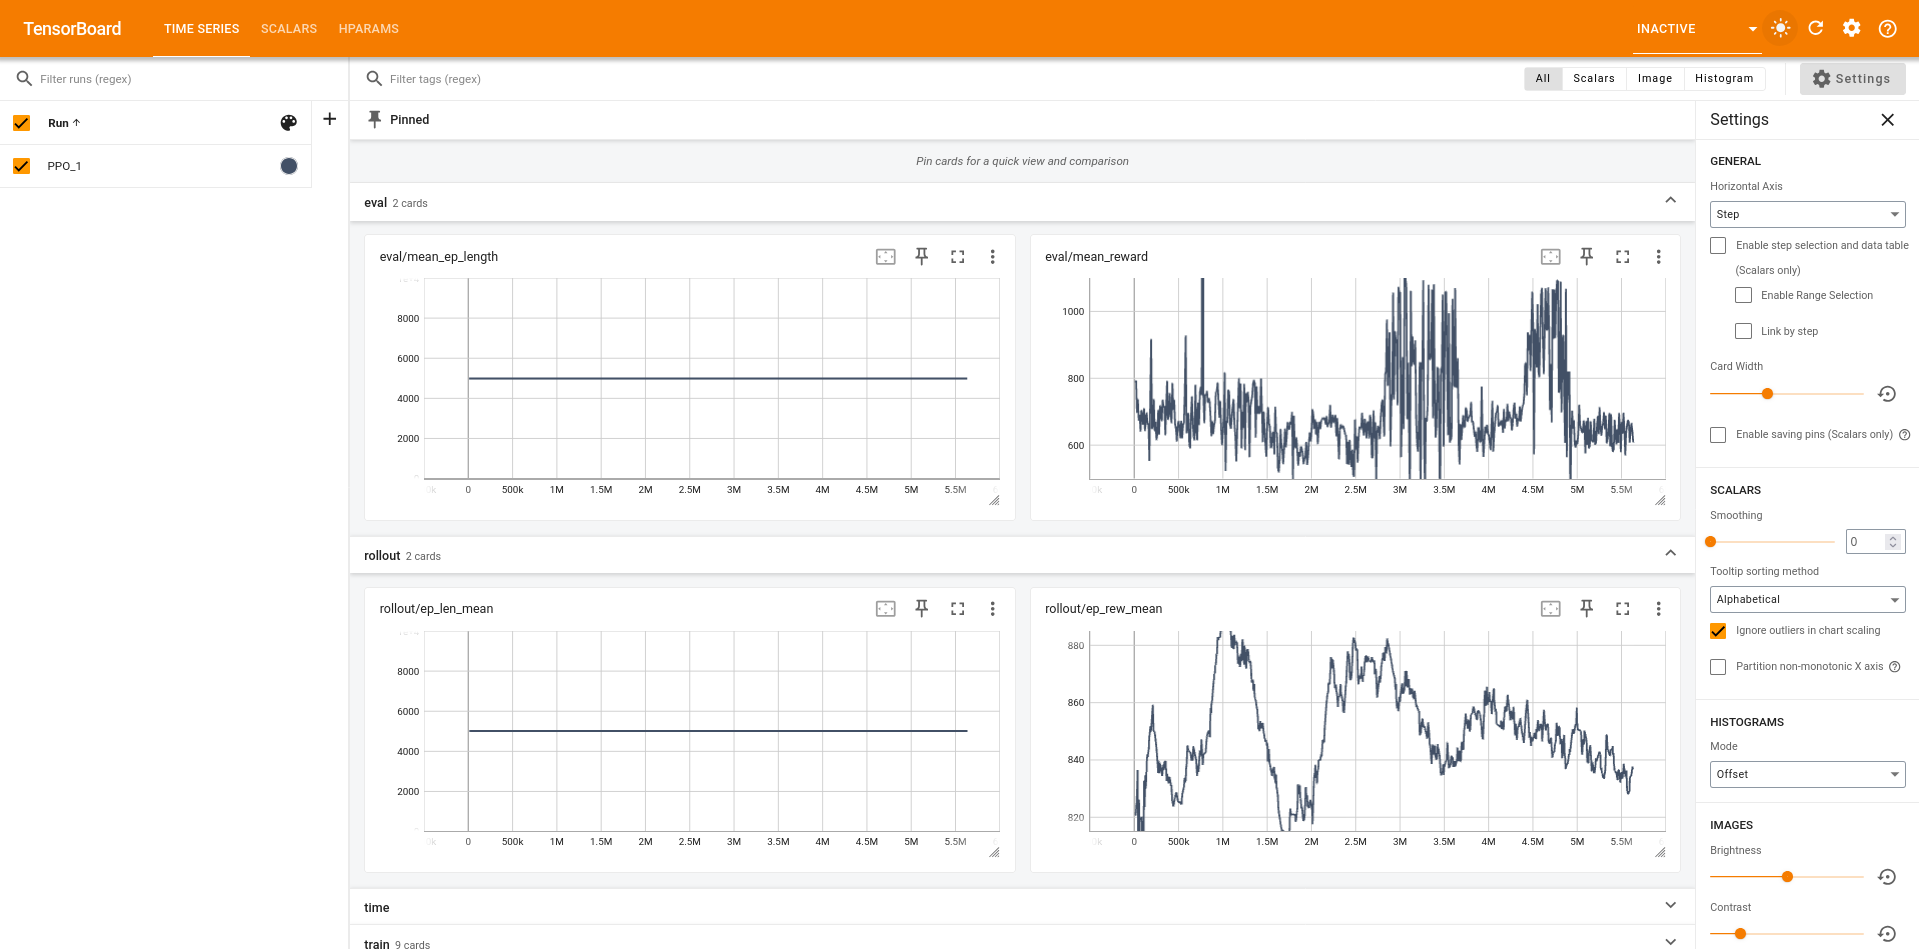
\includegraphics[width=0.98\textwidth, keepaspectratio]{../images/0058 Tensorboard.png}{\\Tensorboard welches ein Training mit PPO zeigt bei dem die mittlere Episodenanzahl konstant ist und die Belohnung im Rollout und in der Evaluation nicht wie gewünscht kontinuirlich steigt.}
\end{center}

\subsection{Zustandsobservation mit einer Inertialen Messeinheit}
Eine Inertiale Messeinheit (eng. Inertial Measuring Unit (IMU)) ist ein System welches in der Regel Beschleunigungssensoren und Drehratensensoren, manchmal auch Magnetfeldsensoren zusammenfasst. Die Bündelung der Sensoren hat sich etabliert da Sensorrohdaten aus den genannten Sensoren häufig fusioniert werden, zur Schätzung von Drehlage und linearer, also um den Gravitationsvektor gefilterte, Beschleunigung. Sensortechnologien wie Laufzeit-, Feldstärke- und Winkelmessung oder Inertialsensorik besitzen prinzipiell komplementäre Eigenschaften in Bezug auf Reichweite, Präzision oder Abtastgeschwindigkeit \ref{link:Sensorfusion}.
Komplementär- und Kalman-Filter sind Beispiele für Sensorfusionsalgorithmen. Auch Methoden des tiefen Lernens eignen sich zur Sensordatenfusion \ref{link:DeepLearningStateEstimation}.\\
Mikrocontrollerhersteller veröffentlichen neben Sensorhardware in der Regel auch Beispielprogramme welche das Auslesen und die Sensordatenfusion demonstrieren.\\
STMicroelectronics bietet die Erweiterung X-CUBE-MEMS1 an welche mit der Bibliothek MotionFX genutzt werden wird zur Sensorfusion \ref{X-CUBE-MEMS1}.

\subsection{Pulsweitenmodulation und Motoransteuerung}
Pulsweitenmodulation (PWM) ist ein Verfahren zur Signalmodulation. PWM-Signale werden unter anderen verwendet zur Ansteuerung von BLDC-Motoren.\\
Bausteine einer mikrocontrollerbasierten Pulsweitenmodulation sind ein Timer und eine Capture/Compare Einheit welche eine Ganzzahl (eng. integer) $n$ hochzählt und mit einem Wert im Capture-Compare-Register (CCR) vergleicht (eng. compare). Ist der Wert des Zählers größer als der Wert im Register wird die Spannung am Output auf Ground gezogen. Zu Beginn beziehungsweise Ende von jeder Periode, dessen Länge durch die Frequenz des Timers bestimmt ist, wird die Spannung beispielsweise auf 3.3V gesetzt. 
\begin{align}
	u(t) &= \left\{\begin{array}{ll} 3.3V, & n < CCR\ \text{mit}\ n\in N\ \text{und}\ n\in [0, CCR]\\
		0, &\text{sonst}\end{array}\right. .
\end{align}
Abhängig vom Pegel stellt sich ein Signal ein welches einen Duty-Cycle $d$ hat der dem Quotient aus Pegel und dem höchsten Wert des Capture-Compare-Registers entspricht. 
\begin{align}
	D &= \frac{n}{\max{(CCR)}}
\end{align}
Der artihmetische Mittelwert des PWM-Signals $u(t)$ ist dann proportional zum Duty-Cycle.
\begin{align}
	\bar{u} &= 3.3V\cdot d
\end{align}
BLDC-Motoren werden wegen ihres Aufbaus zur Klasse der Gleichstrommotoren gezählt\\ benötigen aber jeweils um 120° versetzte periodische, stückweise gleichförmige, Signale an den drei Anschlüssen. Diese Signale können mithilfe von PWM-Signalen aus einem Mikrocontroller generiert werden wobei der Duty-Cycle die Leistungsteuerung und damit die Drehmomentregelung des Motors ermöglicht. Da die Leistung von Mikrocontrollerpins auf 3.3V begrenzt ist, werden in der Praxis noch Leistungstransistoren wie MOSFETs oder IGBTs, sowie eine externe Spannungsquelle zwischengeschaltet. Sowohl die Funktion der Signalgeneration für den BLDC-Motor aus auch, die der Leistungselektronik sind in BLDC-Motortreibern integriert, durch welche der Entwicklungsprozess von Anwendungen mit BLDC-Motoren deutlich beschleunigt wird. Der Entwicklungsaufwand reduziert sich auf die Verschaltung des Treibers und die Generation eines PWM-Signal dessen Duty-Cycle das Motordrehmoment steuert.

\subsection{Flask und ThreeJS}
Flask ist eine Python Bibliothek welche das Programmieren von Webanwendungen vereinfacht \ref{link:Flask}. In Kombination mit der Javaskript Bibliothek ThreeJS lassen sich vergleichsweise schnell 3D-Anwendungen für den Browser entwickeln. Im Netz zugänglich ist neben der ThreeJS Dokumentation eine umfangreiche Zusammenstellung von Beispielen.
\begin{center}
	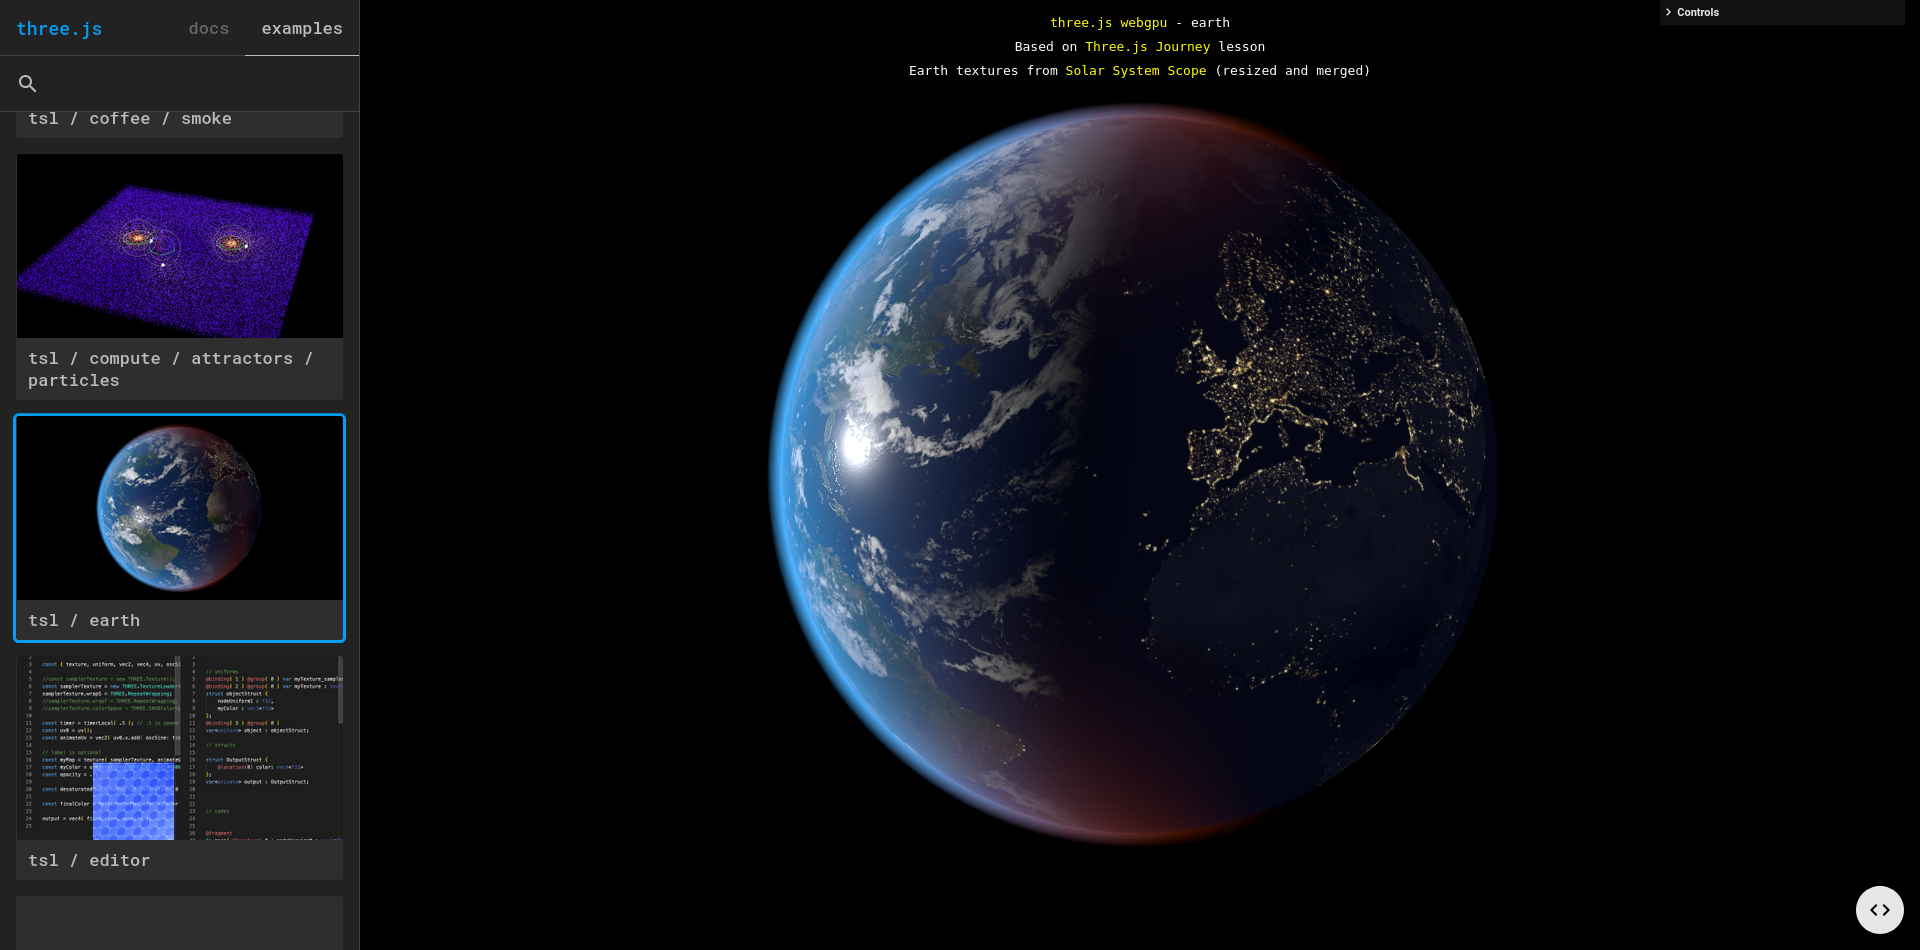
\includegraphics[width=0.9\textwidth, keepaspectratio]{../images/0062 ThreeJS Beispielselektor.png}{\\ThreeJS Beispielselektor mit Beispiel tsl/earth gewählt \ref{bild:3}}
\end{center}

\section{Implementierung}
\subsection{\label{Produktivität}Produktivität und Bellman}
Bei der Implementierung galt es Arbeit daraufhin zu orientieren, dass die Produktivität also das Verhältnis aus Ausbringungsmenge und Arbeitsaufwand maximiert wird \ref{link:Betriebswirtschaftslehre}.\\
Zu Beginn eines jeden neuen Projektes liegen weder ein optimaler Prozessablaufplan noch die zu erwartenden Prozessschrittzeiten vor. Ohne Sicherheit über die Prozessschrittzeiten kann auch keine realistische Gesamtprozesszeit ermittelt werden. Diese Unsicherheiten über das bevorstehende Unterfangen stehen im direkten Widerspruch zur Anforderung nach maximaler Produktivität da diese in der Regel auf Basis von ebensolchen Informationen passiert. Auch gegen Ende eines Projektes lässt sich nur auf Basis von einem Sample ein optimaler Prozessablaufplan abschätzten. Selbst eine mehrfache Wiederholung des Projekts würde nur insignifikante Erkenntnisse bringen da zu erwarten ist, dass die neuen Pläne an den alten orientiert sind. Ob die eigene Herangehensweise an ein Projekt sinnvoll ist kann bei diesen Bedingungen nicht determiniert werden.\\
Um auf Basis von unvollständiger Information dennoch während des Projekts Aussagen über die Produktivität treffen zu können und um diese zu optimieren wurde Bellmans\\ Optimalitätsbedingung \ref{link:DeepReinforcementLearning} als Inspirationsquelle herangezogen. Dieses sagt aus, dass Optimalität in bestimmten Prozessen dann gegeben ist, wenn alle Teilprozess optimal verlaufen. Laufen also beispielsweise alle Teilarbeitsschritte der Quadcopterentwicklung so schnell wie physikalisch möglich dann ist auch die Gesamtentwicklung optimal verlaufen, solange das gesetzte Ziel minimaler Arbeitszeitaufwand ist und kein Teilprozess irrelevant waren. Aus diesem Gedanken lassen sich Handlungsempfehlungen ableiten zur Optimierung bei unvollständiger Information über den vorliegenden Prozess. Zum einen müssen unnötige Arbeiten minimiert werden. Und zum anderen müssen zwingend notwendige Arbeiten optimal durchgeführt werden. Man mag meinen diese Analyse drehe sich im Kreis, doch tatsächlich ist diese Perspektive aussagekräftiger als die Initiale. Denn nun lässt sich sicher sagen, dass die Optimierung von Teilprozessen immer dann Produktivitätsgewinne mit sich bringt, wenn garantiert ist, dass keiner der Teilprozess unnötig ist. Mit der Nebenbedingung, dass der Optimierungsaufwand nicht den Optimierungsertrag übersteigt.\\
Für die Quadcopterentwicklung wurde in jedem Arbeitsschritt einzig und allein auf diesen fokussiert. Operationell wurden Programme, Hardwarearbeiten und Tests isoliert bearbeitet und die strategische Ebene spielte keine Rolle. Es wurde sogar so weit gegangen, dass auch parallel Prozess unabhängig voneinander bearbeitet und nicht aufeinander abgestimmt wurden. Parameter konnten gelernt und unabhängig vom Prototypen entwickelt werden. Auf Interfacekopatibilität wurde nicht geachtet da die Anpassung verschiedener Quadcoptersysteme aneinander als ein kontinuierlicher unausweichlicher Ablaufprozess betrachtet wurde. Durch die Anpassung als separaten Schritt kann insgesamt die Forderung nach einer minimalen Anzahl an unnötigen Arbeitsschritten leicht erreicht werden. Behandelt man Projekte nach diesem Prinzip ist jeder Arbeitsschritt notwendig, um ein gesetztes Ziel zu erreichen. Optionale Schritte gibt es nicht und die zu Verzögerungen werden reduziert auf die Summe der Verzögerungen der einzelnen Arbeitsschritte, welche gut zu fassen sind. Verzögerungen aufgrund von fehlender interner Kommunikation und Informationsmangel werden weitestgehend eliminiert. Es handelt sich zusammenfassend also um eine praktisch orientierte Herangehensweise, welche ohne Projektmanagement auskommt und wert auf Filterung nichtrelevanter Aufgaben legt.

\subsection{Idealer Ablaufplan der gesamten Systemintegrationsprozesses}
Der folgende ideale Ablaufplan wurde im Sinne der Erwägungen aus dem vorangegangenen Abschnitt entwickelt. Alle Schritte sind zwingend erforderlich um den Quadcopter, wie beabsichtigt, mit allen Funktionen, sicher in die Luft zu bringen.
\begin{enumerate} 
	\item Beschaffung
    \item Rahmenproduktion
    \item Montierung und Anbindung der BLDC-Motoren und Treiber
    \item Entwicklung Simulations- und Lernsoftware
    \item Lernen von PID-Parametern
    \item Lernen eines Ende-zu-Ende Modells
    \item Implementierung des Reglers
    \item Produktion der Testbench
    \item Adaption bis der Quadcopter sicher fliegt 
\end{enumerate} 
Bis auf wenige Ausnahmen ist die Ausführungsreihenfolge der Arbeitsschritt irrelevant, weil viele Schritte unabhängig voneinander bearbeitet werden können.\\
Bei der Entwicklung der Mikrocontrollersoftware kam es zu Verzögerungen. Schlussendlich wurde die Architektur nicht wie geplant mit Zephyr sondern in ST implementiert. Doch wirkte sich die Verzögerung kaum auf andere Arbeitsschritte aus. In der Praxis hat sich das Prinzip aus Kapitel \ref{Produktivität} bewährt. Zwar lässt sich auch zum Projektabschluss nicht sagen wie produktiv tatsächlich gearbeitet wurde. Aber Basis von Erfahrungen während des Projekts und mit vorangegangen Projekten ist anzuzweifeln, dass klassischen oder agiles Projektmanagement zu mehr Produktivität geführt hätte, sodass die getroffenen Aussagen zumindest auf Erfahrungswerten fundiert ist.
\subsection{\label{Beschaffung}Beschaffung}
Die Entwicklung des Quadcopters setzt voraus, dass alle Komponenten vorhanden sind. Es stellt sich, die Frage welche Teile benötigt werden. Bei einem technischen System mit einem Teil ist die Frage trivial zu beantworten. Es muss ein Teil beschafft werden, und zwar das System selbst. Ist das System zweiteilig gilt es sicherzustellen, dass Teil 1 zu Teil 2 kompatibel ist und beide beschafft werden. Bei Systemen mit drei Teilen wird es interessant, denn man könnte meinen drei Vergleiche sind notwendig. Doch das muss nicht zwingend der Fall sein. Gibt es zwischen zwei Teilen keine Impuls-, Energie- oder Informationsschnittstelle müssen die Teile nicht auf Kompatibilität überprüft werden. Stehen beispielsweise zwei Schrauben nicht in mechanischem Kontakt müssen Sie in der Regel nicht aufeinander abgestimmt werden. Müsste man jedes Teil mit jedem überprüfen würden die Vergleichskosten fakultativ wachsen
\begin{align}
	\text{Vergleichskosten} &= (\text{Teileanzahl} - 1)!
\end{align}
und damit deutlich schneller als Exponentiell.\\
Das Suchproblem, wie man Teilpaare welche auf Kompatibilität geprüft werden müssen identifiziert stellt sich. Alternativ könnte man auch das Gegenteil fragen, also welche aus allen möglichen Teilen müssen nicht verglichen werden, aber meistens ist es einfacher notwendige Überprüfungen zu finden.\\
Eine mögliche Lösung ist über die Schnittstellen auf Teilpaare zu schließen. Bei der Quadcopterentwicklung wurde dieser Ansatz gewählt und Schnittstellen wurden identifiziert.\\
Weiß man auf welche Teile zu achten ist, kann man mit dem Bestellvorgang beginnen. Doch stellt sich in der Praxis ein weiteres Suchproblem heraus. Und zwar führen Probleme zwischen Teilen in der Regel zu mehr Arbeitsaufwand, weil ein neuer Teilkandidat in Erwägung gezogen werden muss und im ungünstigsten Fall kommt es zu Retouren und ein neues Teil muss beschafft werden, welches potenziell wieder nicht kompatibel ist. Das Suchproblem ist herauszuarbeiten von welchen Teilen ausgehend und in welcher Folge Kompatibilität zwischen Teilen überprüft werden soll damit der Vergleichsaufwand minimal wird. Eine sinnvolle Heuristik ist zunächst das Teil mit den meisten Schnittstellenparametern auf Kompatibilität hin zu überprüfen. Dann alle Teile, welche eine Schnittstelle zum vorangegangenen Teil aufweisen überprüfen, wobei wiederum Teile mit vielen Schnittstellenparametern priorisiert werden.\\
Selbst für überschaubare System wie einen Quadcopter können diese theoretischen Handlungsempfehlungen Zeit und Nerven bei der Beschaffung sparen.\\
Da der Quadcopterrahmen die meisten Schnittstellen zu anderen Teilen aufwies wurden ausgehend von ihm Teile beschafft.\\
Zentrales Bauteile ist neben den BLDC-Motoren und dem Rahmen das Herzstück des Quadcopters der Rechner, auf welchem die Regelung prozessiert wird.
Um diese Aufgabe zu erfüllen wurde ein ST NUCELO-F411RE \ref{link:33} ergänzt durch ein X-NUCLEO-IKS4A1Sensorboard\\ beschafft \ref{link:34}.
\begin{center}
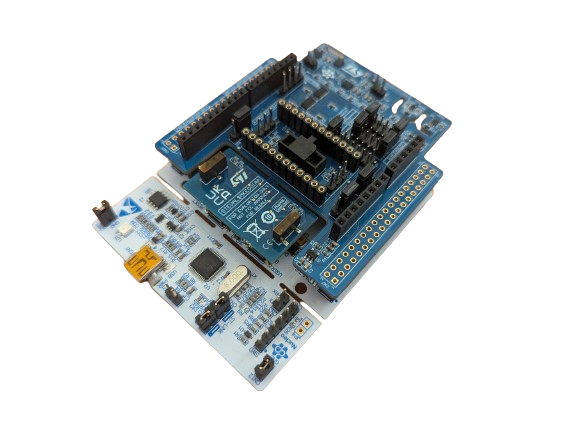
\includegraphics[scale=0.6]{../images/0002 nucleo-f411re.png}{\\STMicroelectronis NUCLEO-F411RE Mikrocontrollerboard mit X-NUCLEO-IKS4A1 Sensorboard}
\end{center}
Die Beschaffung aller Teile lief, bis auf ein überdimensioniertes Kabel und unterdimensioniert Propeller und Motoren reibungslos.\\
Allerdings war der ST NUCELO-F411RE nicht die erste Wahl. Zunächst wurde ein STM32-F4-DISCO bestellt. Da mit diesem aber keine serielle Verbindung zum Rechner aufgebaut werden konnte hatte das NUCLEO-F411RE Board die Möglichkeit sich, als würdigen Ersatz zu präsentieren. Dieser Fehler ist nicht als Beschaffungsfehler klassifiziert, sondern als Produktfehler.
\subsection{Rahmenproduktion}
Neben den Empfehlungen aus \ref{Beschaffung} hat sich auch herauskristallisiert, dass es hilft Teile zu haben, welche adaptiv sind. Der gewählte Rahmen wurde mit Teilen aus einem Baukasten der Firma Totem produziert, welche flexibel sind. Beispielsweise konnte die Rahmengeometrie oder -stärke schnell und ohne Beschaffungskosten angepasst werden. Technisch gesehen muss der Rahmen also nicht als Elementarteil, sondern schon als Produkt bezeichnet werden.
\subsection{Montierung und Anbindung der BLDC-Motoren und Treiber}
Die mechanische Schnittstelle zwischen dem Rahmen und den BLDC-Motoren muss mindestens alle nominal auftretenden Impulsströme leiten können. Nominale Zustände sind solche die beim Flug mit bis zu 30m/s und Starts- und Landungen mit bis zu 0.5m/s auftreten.\\
Die Verbindung wurde realisiert mit Bauteilen und 3mm-Schrauben aus dem Totem-Baukasten. Das Anlegen von Kraft orthogonal zum Rahmenarm offenbarte, dass die Verbindung zwischen Motor und Rahmen solide ist. Auch deutlich wurde aber, dass der Rahmen in ebendiese Richtung vergleichsweise leicht biegsam ist. Um dem entgegenzuwirken wurden für den zweiten Prototypen Querverstrebungen angeschraubt. Das Problem konnte dadurch gelöst werden zum Preis von etwas mehr Gewicht.

\subsection{\label{software:Software}Entwicklung der Simulations- und Lernsoftware}
\subsubsection{Analyse und Adaption der Quadcopterdynamik}
Die Simulationssoftware welche für die Reglerentwicklung wurde so ausgewählt und in Teilen entwickelt, dass Sie mit beliebigen Parameter funktioniert. Die Informatinen aus den vorangegangen Kapiteln mussten also nicht vorliegen für die Entwicklung der Simulationssoftware. Die folgenden Parameter sind jene die für den Großteil der Simulationen verwendet wurden. Ein wichtiger offener Punkt ist nach wie vor die Angleichung der Parameter an den Prototypen, sowie die Simulation und das Training von Reglern mit den realen Parameter. Anschließend kann die Kompatiblität des Modells zum Quadcoptersystem getestet werden. Offen geblieben sind die Punkte, da der Fokus auf der Entwicklung anderer System lag und das Training der PID-Parameter nicht wie Anfangs erwartet in einem Monat abgeschlossen werden konnte.
\vspace*{0.5cm}
\begin{center}
\begin{tabular}[h]{|l|l|l|l|l|}
\hline 
System & Komponenten & Modellparameter & Wert & Quelle \\
\hline 
Gesamt & Quadcopter & $m$ & $\approx $0.94kg & \\
& & $I_{B,xx}$ & 1.23e-2$\frac{kg}{m^2}$ & \ref{link:SimCon}\\
& & $I_{B,yy}$ & 1.23e-2$\frac{kg}{m^2}$ & \ref{link:SimCon}\\
& & $I_{B,zz}$ & 2.24e-2$\frac{kg}{m^2}$ & \ref{link:SimCon}\\
\hline
Impulsfluss & Propeller, Motor & $\tau$ & 0.1 & \ref{link:SimCon}\\
& & d & 1 (Keine Dämpfung)  & \ref{link:SimCon} \\
& & $k_p$ & 1 & \ref{link:SimCon} \\
& & $k_{Th}$ & 1.076e-5$\frac{Ns^2}{rad^2}$ & \ref{link:SimCon}\\
& & $k_{To}$ & 1.632e-7$\frac{Nms^2}{rad^2}$ & \ref{link:SimCon}\\
& Rahmen & $l$ & 0.25m & \\
& & $w$ & 0.25m & \\
& & $h_M$ & 0.05m & \\
\hline
Energiefluss & Akkumulator & $u_{max}$ & 7.4V & \ref{Akku}\\
& & $i_{max}$ & 40A & \ref{Akku}\\
& BLDC-Treiber & $u_{soll, gelb}$ & PWM(60Hz, 80\%-90\%) & \ref{link:Treiberdatenblatt}\\
& & $u_{soll, rot}$ & 5V & \ref{link:Treiberdatenblatt}\\
& & $u_{soll, braun}$ & 0V & \ref{link:Treiberdatenblatt}\\
\hline
\end{tabular}
\end{center}
\vspace*{0.5cm}
Für das Anlernen von Strategien sind dynamische Simulationen der Umwelt unabdingbar. Funktionen zur Quadcopterdynamiksimulation wurden aus dem Repository von John Bobzwik \ref{simcon:simcon} übernommen, wobei darauf zu achten war, dass die beigefügte Lizenz den Einsatz erlaubt.\\
Die Methode \textit{update} berechnet den nächsten Zustandsvektor des Quadcopters bei der in \textit{config.py} definierten Schrittweite. Der Vektor Zustand entspricht dem Zustandsvektor \ref{zustandsvektor:zustandsvektor} und in jedem Schritt aktualisiert. 
\begin{center}
\begin{tikzpicture}[font=\sffamily,every label/.append
style={font=\small\sffamily,align=center}]

\node[doc, fill=white] (Quadcontroller) {quad.py\\  \begin{lstlisting}[language=Python, basicstyle=\fontsize{8}{10}\selectfont]
...
def zustandsaenderung(self, t, zustand, motorbefehle, wind):
...

	# Differenzialgleichungen
	wddotM1 = (
		-2.0 * self.damp * self.tau * wdotM1 - 
		wM1 + 
		self.kp * motorbefehle[0]
	) / (self.tau ** 2)
	...
	
	wMotor = numpy.array([wM1, wM2, wM3, wM4])
	wMotor = numpy.clip(
		wMotor, 
		self.minWmotor, 
		self.maxWmotor
	)
	schub = self.kTh * wMotor * wMotor
	drehmoment = self.kTo * wMotor * wMotor
	
	# Inertialtensor
	IBxx = self.IB[0, 0]
	IByy = self.IB[1, 1]
	IBzz = self.IB[2, 2]
	
	MM * sdotn = RHS
	sdot = inv(MM) * RHS
	
	# Schrieben von wddot in sdot
	...
	
	self.beschleunigung = sdot[7:10]
	
	return sdot

def update(self, t, cmd, wind):
	geschwindigkeit_t_minus_1 = self.zustand[7:10]
	omega_t_minus_1 = self.zustand[10:13]
	
	self.integrator.set_f_params(cmd, wind)
	self.zustand = self.integrator.integrate(
		t, 
		t + config.Schrittweite
	)
	
	self.pos = self.zustand[0:3]
	self.quat = self.zustand[3:7]
	self.geschwindigkeit = self.zustand[7:10]
	self.omega = self.zustand[10:13]
	self.wMotor = numpy.array([
		self.zustand[13], 
		self.zustand[15], 
		self.zustand[17],
		self.zustand[19]
	])
	
	self.vel_dot = (
		self.geschwindigkeit - geschwindigkeit_t_minus_1
	) / config.Schrittweite
	self.omega_dot = (
		self.omega - omega_t_minus_1
	) / config.Schrittweite
	
	...
...
\end{lstlisting}
};
\end{tikzpicture}
\end{center}
Die Methode \textit{update} berechnet aus den Motorbefehlen, welche in der Einheit $rad/s$ vorliegen und optionalen Windparametern den nächsten Zustand.

\subsubsection{Architektur}
Zum Erreichen des Ziels der Quadcopterentwicklung wurden eine Reihe an lose gekoppelten Softwareanwendungen, welche teilweise autonom aber auch als Verbund operieren können, programmiert. In einem Repository Quadstar sind alle Daten und Programme zusammengefasst.
\begin{center}
	\begin{tikzpicture}[font=\sffamily,every label/.append
		style={font=\small\sffamily,align=center}]
		
		\node[doc, fill=white] (Quadcontroller) {./Quadstar/\\  \begin{lstlisting}[language=Python, basicstyle=\fontsize{8}{10}\selectfont] 
Modelle    
config.py       
joystick.py  
quaternion.py      
quad.py       
quadpid.py
quadendezuende.py       
quadlive.py  
quadtest.py        
quadregler.py  
quadseriell.py  
quadtrain.py  
wind.py    
			\end{lstlisting}
		};
	\end{tikzpicture}
\end{center}
Die Programmbeziehungen wurden visuell aufbereitet.
\begin{center}
	\begin{tikzpicture}[font=\sffamily,every label/.append
		style={font=\small\sffamily,align=center}]
		
		\node[doc, fill=green] at (-2, 1) (Quad) {quad.py};
		
		\node[doc, fill=green] at (-2, 3) (Quadlive) {quadlive.py};
		
		\node[doc, fill=green] at (-1, 5) (Quadtest) {quadtest.py};
		
		\node[doc, fill=green] at (-1, -1) (Quadserial) {quadserial.py};
		
		\node[doc, fill=green] at (2, 6) 
		 (Quadcontroller) {quadcontroller.py};

		\node[doc, fill=green] at (6, 3) (Quadmodel) {quadendezuende.py};

		\node[doc, fill=green] at (5, 5) (Quadpid) {quadpid.py};
		
		\node[doc, fill=blue!50] at (10, -2) (Quadsoft) {quadsoft.c};

		\node[doc,fill=blue!50] at (6, -7) (quadsoft) {quadsoft};

		\node[doc, fill=green, minimum width=2cm,minimum height=1cm] at (6, 1) (Config) {config.py};

		\node[doc, fill=green, minimum width=2cm,minimum height=1cm] at (5, -1) (Joystick) {joystick.py};

		\node[doc, fill=green, minimum width=2cm,minimum height=1cm] at (2, -2) (Quaternion) {quaternion.py};
		
		\draw[-latex] (Config.west) .. controls +(left:7mm) and +(left:7mm) .. (Quadpid.west);

		\draw[-latex] (Config.west) .. controls +(left:7mm) and +(left:7mm) .. (Quadmodel.west);

		\draw[-latex] (Config.west) .. controls +(left:7mm) and +(right:7mm) .. (Quadtest.east);

		\draw[-latex] (Config.west) .. controls +(left:7mm) and +(right:7mm) .. (Quad.east);

		\draw[-latex] (Config.west) .. controls +(left:7mm) and +(left:7mm) .. (Joystick.west);

		\draw[-latex] (Quadserial.east) .. controls +(right:7mm) and +(left:7mm) .. (Joystick.west);

		\draw[-latex] (Config.west) .. controls +(left:7mm) and +(right:7mm) .. (Quadserial.east);

		\draw[-latex] (Quad.east) .. controls +(right:7mm) and +(left:7mm) .. (Quadpid.west);

		\draw[-latex] (Config.west) .. controls +(left:7mm) and +(right:7mm) .. (Quadlive.east);

		\draw[-latex] (Quaternion.north) .. controls +(up:7mm) and +(right:7mm) .. (Quadlive.east);

		\draw[-latex] (Quadserial.east) .. controls +(right:7mm) and +(right:7mm) .. (Quadlive.east);

		\draw[-latex] (Quaternion.north) .. controls +(up:7mm) and +(right:7mm) .. (Quadtest.east);

		\draw[-latex] (Quad.east) .. controls +(right:7mm) and +(right:7mm) .. (Quadtest.east);

		\draw[-latex] (Quad.east) .. controls +(right:7mm) and +(left:7mm) .. (Quadmodel.west);

		\draw[-latex] (Quaternion.north) .. controls +(up:7mm) and +(left:7mm) .. (Quadmodel.west);

		\draw[-latex] (Quaternion.north) .. controls +(up:7mm) and +(right:7mm) .. (Quad.east);

		\draw[-latex] (Quadcontroller.south) .. controls +(down:7mm) and +(right:7mm) .. (Quadtest.east);

		\draw[-latex] (Quaternion.north) .. controls +(up:7mm) and +(left:7mm) .. (Quadpid.west);

		\draw[-latex, dash pattern=on 10pt off 5pt] (Quadserial.south) .. controls +(down:25mm) and +(up:20mm) .. (quadsoft.north) node[midway, left,font=\small\sffamily]{Sollgeschwindigkeit};

		\draw[-latex, dash pattern=on 10pt off 5pt] (Quadsoft.south) .. controls +(down:20mm) and +(up:20mm) .. (quadsoft.north);

		\draw[-latex] (Quad.east) .. controls +(right:7mm) and +(right:7mm) .. (Quadlive.east);
		
		\node[draw,dashed,rounded corners,fit=(Quadsoft),inner
		xsep=10pt,inner ysep=30pt,label={above:{STM32CubeIDE}}](fit3){};

		\node[draw,dashed,rounded corners,fit=(Quadlive) (Quadtest) (Quadserial) (Quadcontroller) (Quadmodel) (Quadpid) (Quaternion) (Quad) (Config),inner
		xsep=10pt,inner ysep=30pt,label={above:{Visual Studio Code}}](fit4){};

		\node[draw,dashed,rounded corners,fit=(fit3) (fit4),inner
		xsep=10pt,inner ysep=30pt,label={above:{Thinkpad P52s}}](fit4){};
		
		\node[parallelepiped,draw=yellow,fill=red!80,
		minimum width=2cm,minimum height=1.5cm,align=center,text=white] at (0, -7) (imu) {IMU};
		
		\node[right=1.5cm of quadsoft, doc, fill=yellow, minimum width=2cm, minimum height=1cm] (HTML) {PWM, CCR};
		
		\draw[-latex] (imu) -- (quadsoft) node[midway, above, font=\small\sffamily]{Messwerte};
		
		\draw[-latex] (quadsoft) -- (HTML) node[midway, below, font=\small\sffamily]{Befehle};
		
		\draw[-latex, dash pattern=on 10pt off 5pt] (quadsoft.north) .. controls +(up:25mm) and +(down:20mm) .. (Quadserial.south) node[midway, right,font=\small\sffamily]{Messwerte};
		
		\draw[-latex] (Quad.east) .. controls +(right:7mm) and +(down:7mm) .. (Quadcontroller.south) node[midway, right, font=\small\sffamily]{};
		
		\node[draw,dashed,rounded corners,fit=(quadsoft) (HTML),inner
		sep=10pt,label={above:{NUCLEO-F411RE}}](fit4){};
		
		\node[draw,dashed,rounded corners,fit=(imu),inner
		sep=10pt,label={above:{X-NUCLEO-IKS4A1}}](fit5){};
		
	\end{tikzpicture}
\end{center}
Alle Python Dateien enthalten eine Klasse und instanziieren mindestens eine andere Klasse. Neben den Python Dateien welche mit Visual Studio Code entwickelt worden sind, wurde das Reglerprogramm mit C in der STM32CubeIDE geschrieben.
Das Diagramm visualisiert Klassen welche andere instanziieren und Informationsflüsse über eine serielle Schnittstelle mit Pfeilen. Ein Pfeil von einer Python Datei zu einer anderen bedeutet letztere Python Datei arbeitet mit erster. Gestrichelte Pfeil stellen Informationsfluss über UART dar.\\
Die in \textit{quad.py} definierte Klasse Quadcopter umfasst vor allem die Quadcopterdynamiksimulation \ref{simcon:simcon}. Mit \textit{quadtrain.py} welche Methoden aus \textit{quadpid.py} oder \textit{quadendezuende.py} aufruft lassen sich PID-Parameter beziehungsweise Ende-zu-Ende-Modelle lernen. 
Die Klassen \textit{Quadpid} und \textit{Quadendezuende} welche in \textit{quadpid.py} beziehungsweise \textit{quadendezuende.py} definiert sind erben von \text{gym.Env} \ref{gymnasium} und implementierten die Funktionen \textit{reset} und \textit{step}. Trainiert der Nutzer ein Modell mit \textit{quadtrain.py} greift Stable Baselines3 auf eine der Umwelten zu entsprechend der Definition in \textit{config.py}. Weiterführende Details zur Implementierung, Spezifizierung und zu den Hyperparametern der Trainingsumgebungen werden in \ref{pidlernen} und \ref{EndeZuEndeModell}\\ vorgestellt. Durch den Aufruf von \textit{quadlive.py} wird ein Flask-Server gestartet mithilfe von welchem die Trajektorie eines Quadcopter im Browser simuliert wird. 
\begin{center}
	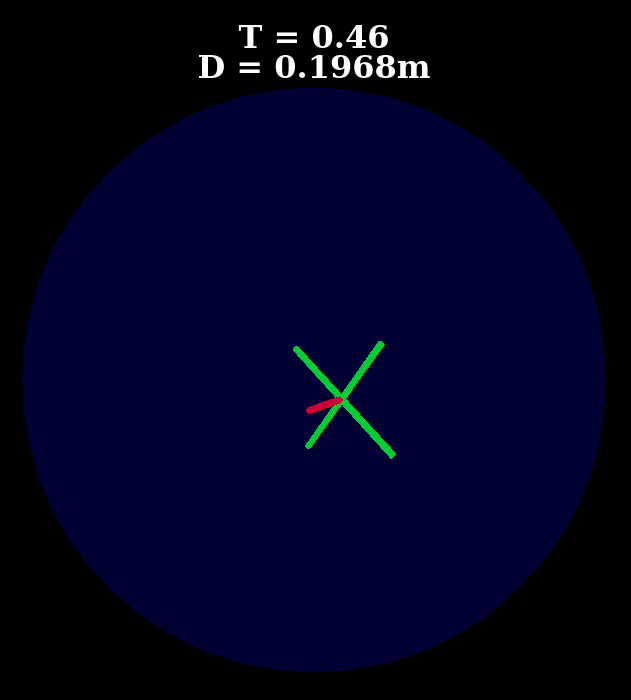
\includegraphics[scale=0.3]{../images/0068 Quadlive 1.png}{\\Visualisierung des Quadcopters mit \textit{quadlive.py} im Browser}
\end{center}
Die Webvisualisierung greift auf Methoden aus \textit{quadtest.py} zurück welche auch dazu verwendet werden können, Plots von Trajektorien zu erstellen. Gezeichnet werden 6 translatorischen Parameter welche die Position und Geschwindigkeit des Quadcopters im Nord-Ost-Unten Orientierungssystem repräsentieren und 3 rotatorische Parameter, welche die Drehlage darstellen, wobei die Darstellung in Polarkoordinaten gewählt wurde, um der periodischen Natur der Größe gerecht zu werden.\\
Die Entwicklung und Implementierung des Programms \textit{quadsoft.c}, auf dem NUCELO-F411RE Board, ist Teil des Arbeitsschrittes Reglerimplementierung \ref{Reglerimplementierung:Reglerimplementierung}.\\
Hervorzuheben ist die \textit{config.py} Datei, da in ihr alle relevant Parameter zum Einstellen des Programmverhaltens zusammengefasst sind. Daneben hat die Datei die Funktion Modellbeschreibungsdateien, welche beim Training in den Modellordner kopiert werden, zu leiten. Will der Nutzer ein trainiertes Modell testen kann er einfach die Konfigurationsdatei in das Hauptverzeichnis kopieren, wodurch das Programm dieses erkennt und anwendet, sofern der Nutzer keine Änderung an der Bezeichnung vorgenommen hat. In Zukunft ist denkbar, die Configuration kann vom Nutzer wegzuabstrahieren wodurch allerdings potenziell eine Freiheitseinschränkung mit einhergehen könnte. Die wichtigsten Parameter werden kurz beschreiben.
\vspace*{0.5cm}
\begin{center}
	\begin{tabular}[h]{|c|c|c|c|}
		\hline 
		Konfigurationsparameter & Typischer Wert & Bedeutung\\
		\hline
		Umweltparameter & & \\
		Schrittweite & 1e-3 & Schrittweite in s\\
		Finaler Zeitpunkt & 1s & Simulationsende in s\\
		Initaler Zeitpunkt & 0s & Simulationsbeginn in s\\
		\hline 
		Quadtrain & & \\
		Ordnername & QM-01-01-2024-SC42-A & Modellordner\\ 
		Episoden & 1e8 & Episodengesamtzahl \\
		Actor & [2, 2] & Schichtentopologie Actor\\
		Critic & [2, 2] & Schichtentopologie Critic\\ 
		Lernrate ($\alpha$) & 1e-4 & Lernrate \\
		Parallele Umwelten & 4 & siehe \ref{paralleleUmwelten}\\
		Batchmenge & 16 & Batchmenge\\
		\hline 
		Quadendezuende & &\\
		Aktionsraum Datentyp & float32 &\\
		Aktionsraum EndeZuEnde & [0$\frac{rad}{s}$ bis 1000$\frac{rad}{s}$] & siehe \ref{EndeZuEndeModell}\\
		Belohnungsgewichtung & [0.0, 0.4, 0.2, 0.4] & siehe \ref{Belohnung}\\
		\hline
	\end{tabular}
\end{center}
Der Ordnername, im Beispiel QM-01-01-2024-SC42-1, setzt sich zusammen aus einem Reglerbezeichner, dem Datum im Format Tag, Monat und Jahr, einem Hardwarebezeichner und abschließend einer Identifikationsnummer. Der Reglerbezeichner QM steht für Ende-zu-Ende-Modelle. PID-Regler wurden mit QP bezeichnet. Das Datum markiert den Tag, an dem mit dem Training des Modells begonnen wurde und der Identifikationsbuchstabe unterscheidet Modelle eines Tages, sodass diese bei Modellen mit unterschiedlichem Datum dieselbe sein kann.

\subsubsection{\label{Belohnung}Belohnungsfunktionen}
Die Belohnungsfunktion ist inspieriert von \ref{link:ReinforcementLearningQuadcopter}. \\
Der Nutzer kann vier Belohnungsfunktionen gewichten.
Diese berechnen die Belohnung positionsbasiert
\begin{align}
r_p(x, y, z) &= \frac{1}{1 + (x - x_{soll})^2 + (y - y_{soll})^2 + (z - z_{soll})^2}
\end{align}
lagebasiert
\begin{align}
r_{\varphi}(\phi, \theta, \psi) &= \frac{1}{1 + (\phi - \phi_{soll})^2 + (\theta - \theta_{soll})^2 + (\psi - \psi_{soll})^2}
\end{align}
geschwindigkeitsbasiert
\begin{align}
r_v(v_x, v_y, v_z) &= \frac{1}{1 + (v_x - v_{x, soll})^2 + (v_y - v_{y_soll})^2 + (v_z - v_{z, soll})^2}
\end{align}
und drehratenbasiert
\begin{align}
r_{\dot{\varphi}}(\dot{\phi}_x, \dot{\theta}_y, \dot{\psi}_z) &= \frac{1}{1 + (\dot{\phi} - \dot{\phi}_{soll})^2 + (\dot{\theta} - \dot{\theta}_{soll})^2 + (\dot{\psi} - \dot{\psi}_{soll})^2}.
\end{align}
Die Gewichtung erfolgt mit 4 Parametern 
\begin{align}
r &= \alpha_r r_p + \beta_r r_v + \gamma_r r_{\varphi} + \delta_r r_{\dot{\varphi}}.
\end{align}
Die Summe der Parameter
\begin{align}
\alpha_r + \beta_r + \gamma_r + \delta_r &= 1 
\end{align}
sollte immer Eins sein um Vergleichbarkeit herzustellen.
Die Autoren von \ref{link:ReinforcementLearningQuadcopter} beobachteten eine starke Abhängigkeit der Lernperformance von der Wahl der Parameter. Da für den Quadcopter ein Geschwindigkeitsregler implementiert werden soll, spielt die Positionsbelohnung $r_p$ nur eine untergeordnete Rolle.\\
Bei der vorgestellten Belohnungsfunktion handelt es sich nicht um die einzige verwendete.

\subsubsection{Beobachtungsraum}
Die Beobachtung enthält die Ist- und die Sollgeschwindigkeit sowie die Drehlage, welche aus der Quaternionen des Zustandsvektors $s$ berechnet wird. Zunächst wurde der Beobachtungsraum ohne die Istgeschwindigkeit aufgestellt. Da mit diesem Setup kein Modell lernte wurde Sie testweise hinzugenommen und praktisch ein Problem aus dem Bereich des Überwachten Lernens \ref{link:MaschinellesLernen} zu einem des Tiefen Verstärken Lernens gemacht. Ob das Sinnvoll ist wird nicht weiter elaboriert. Mit dem Setup gelang es aber zumindest kleine Lernerfolge \ref{EndeZuEndeModell} mit Tiefen Verstärkendem Lernen zu erzielen.
\begin{align}
	s_t &= \begin{pmatrix}
		v_3\\
		v_{3, Soll}\\
		\varphi_3
	\end{pmatrix}
\end{align}
In der Simulation werden die Werte für alle Beobachtungen direkt aus dem Zustandsvektor ausgelesen. Bedeutet es wurde kein Sensorrauschen simuliert und auch das Übertragungsverhalten der Sensoren wurde nicht betrachtet. 

\subsubsection{\label{Geschwindigkeitssollvektor}Geschwindigkeitssollvektor}
Der Geschwindigkeitssollvektor welcher für das Training aller PID und Ende-zu-Ende Modelle eingesetzt wurde, enthält 8 Elemente und ermöglicht keine Bewegung auf der Unten-Dimension. Die Unten-Dimension wurde ignoriert da das Lernen von acht Sollgeschwindigkeiten als einfacher erachtet wurde als das Lernen von 27 Dimension.
\begin{align}
	v_{Soll} &= \begin{pmatrix}
		\text{randint}(-1, +1)\\
		\text{randint}(-1, +1)\\
		0
	\end{pmatrix}
\end{align}
Auch mit einem Joystick wurden Sollwerte produziert, als Teil der Testbench \ref{testbench:testbench}. Die zwei Sollwertinterface funktionieren unabhängig voneinander. Wichtig ist nur, dass das Format für das Training dem Format des Quadcopterreglers auf dem Mikrocontroller entspricht.
Im Laufe der Entwicklung unterlief der Geschwindigkeitssollvektor kontinuierlich Anpassungen. Gewählt wurde die Form da Sie auf die Zustände eines Joysticks, ohne Schub passt. Ein Durchdrücken des Joysticks nach vorne rechts entspricht dem Geschwindigkeitssollvektor
\begin{align}
	v_{Soll,Vorne,Rechts} &= \begin{pmatrix}
		1\\
		1\\
		0
	\end{pmatrix}.
\end{align}
Alle weiteren Joystickzustände ergeben sich entsprechend. 

\subsection{\label{pidlernen}Lernen der PID-Parameter}
Durch das Lernen von PID-Parameter kann in der Theorie sowohl die Reglerperformance maximiert werden als auch auf die manuelle Parametersuche verzichtet werden.\\
Das Anlernen des PID-Geschwindigkeitsregelers umfasste bis zu 18 PID-Parameter. Zu beachten ist, dass für die Nord- und Ost-Dimension häufig eine Aktion zwei Parameter bestimmt. Die tatsächliche Zahl der PID-Parameter im Geschwindigkeitsregler ist 24.
\begin{align}
	a_t &= \begin{pmatrix}
		P_{v,3}\\
		I_{v,3}\\
		D_{v,3}\\
		P_{q,3}\\
		P_{\varphi,3}\\
		P_{\dot{\varphi},3}\\
		D_{\dot{\varphi},3}
	\end{pmatrix}
	= \begin{pmatrix}
		P-Geschwindigkeit (Nord, Ost, Unten)\\
		I-Geschwindigkeit (Nord, Ost, Unten)\\
		D-Geschwindigkeit (Nord, Ost, Unten)\\
		P-Drehlage (Quaternion)\\
		P-Drehlage (Rollen, Nicken, Gieren)\\
		P-Drehrate (Rollrate, Nickrate, Gierrate)\\
		D-Drehrate (Rollrate, Nickrate, Gierrate)\\
	\end{pmatrix}
\end{align}
Der Regler berechnet zunächst mithilfe von PID-Geschwindigkeitsregelern einen Sollschubvektor. Dieser Sollschubvektor wird umgerechnet zu einer Solldrehlage welche in Quadternionenfrom Eingang für das Kontrollgesetz ist, vergleich \ref{Quadcopterregelungsproblem}.\\
Die Visualisierung zeigt ein Standard-Regelkreis welcher Teil der Gesamtarchitektur ist die den Regelkreis ergänzt um einen PPO-Agenten und eine Belohnungsfunktion. Verdeutlichen soll die Visualisierung nicht die Softwarearchitektur sondern den Unterschied zwischen der Schrittweite des Regelkreises $n_R$ und der Schrittweite bis der Agent $n_{PPO}$ neue PID-Parameter im PID-Regler setzt. Anfangs wurden verschiedene adaptive Regler trainiert, also solche mit 
\begin{align}
	n_{PPO}\Delta t_{Modell} < n_R\Delta t_{Modell}\cdot \text{Episodenende}
\end{align}
bei denen in einer Episode die PID-Parameter nicht nur einmal zu Beginn gesetzt werden. Spätestens als sich das Problem des Lernens von PID-Parameter als schwerer als erwartet erwiesen hat wurde nicht mehr an adaptiven, kombinierten PID-/PPO-Reglern geforscht. Die Parameter wurden in jeder Episode zu Beginn einmal gesetzt, was einem \textit{step} pro Episode in Famara Gymnasium entspricht.
\begin{center}
\begin{tikzpicture}[font=\sffamily, every label/.append style={font=\small\sffamily, align=center}]

\node[doc] (Regler) {PID-Regler};

\node[right=1cm of Regler, doc] (Umweltmodell) {
	Umweltmodell, $f_U$
};

\node[below=2.3cm of Regler, doc] (Observationsmodell) {
	Observationsmodell
};

\node[left=4cm of Regler, doc] (Sollwertinterface) {
	Sollwertinterface
};

\draw[-latex] (Regler) -- (Umweltmodell) node[above, midway, font=\small\sffamily]{$\omega_t$};

\node[left=2.5cm of Regler, circle, draw] (c) at (0,0) {-}; 

\draw[-latex] (Observationsmodell) -| (c) node[midway, left, font=\small\sffamily]{$s_{t, Mess}$};

\draw[-latex] (c) -- (Regler) node[above, midway, font=\small\sffamily]{$e_t$};

\draw[-latex] (Umweltmodell) |- (Observationsmodell) node[right, midway, font=\small\sffamily]{$y_t$};

\draw[-latex] (Sollwertinterface) -- (c) node[above, midway, font=\small\sffamily]{$s_{Soll}$};

\node[
draw,
dashed,
rounded corners,
fit=(Regler) (Umweltmodell) (Sollwertinterface) (Observationsmodell),
inner sep=10pt,
label={above:{Regelkreis}}
](fit5){};

\node[above=2.6cm of Regler, doc] (PPO) {PPO};

\node[above=1cm of PPO, doc] (Belohnungsfunktion) {Belohnungsfunktion};

\draw[-latex] (Umweltmodell) |- (PPO) node[right, midway, font=\small\sffamily]{$s_{t}$};

\draw[-latex] (Umweltmodell) |- (Belohnungsfunktion);

\draw[-latex] (Belohnungsfunktion) -- (PPO) node[right, midway, font=\small\sffamily]{$r_{t}$};

\draw[-latex] (PPO) -- (Regler)node[right, midway, font=\small\sffamily]{$a_{t}$};

\draw[-latex] (Sollwertinterface) |- (Belohnungsfunktion)node[left, midway, font=\small\sffamily]{$s_{Soll}$};

\node[
	draw,
	dashed,
	rounded corners,
	fit=(Regler) (Umweltmodell) (Sollwertinterface) (Observationsmodell) (PPO) (Belohnungsfunktion) (fit5),
	inner sep=10pt,
	label={above:{Architektur}}
](all2){};


\draw[-latex] (1.8, -1) arc (90:-220:0.8) node[above, font=\small\sffamily]{$f_{R}$};

\draw[-latex] (1.8, 3) arc (90:380:0.8) node[above, font=\small\sffamily]{$f_{PPO}$};

\end{tikzpicture}
\end{center}
\vspace*{0.5cm}
Da nicht auf alle trainierten Modelle eingengangen werden kann wird der Fokus auf den vielversprechensten liegen. Das erfolgversprechenste Modell für PID-Parameter hat die folgende Konfiguration und wurde für 220e3 Episoden trainiert. 
\begin{center}
\begin{tabular}[h]{|c|c|}
\hline 
Konfigurationsparameter & Wert \\
\hline 
Umweltparameter & \\
Schrittweite $\Delta t_{Modell}$ & 1e-3s \\
Episodenende & 1s\\
\hline
Quadtrain & \\
Ordnername & QP-12-09-24-EIPC55-A\\
Lernrate $\alpha$ & 1e-4\\
Parallele Umwelten & 4\\
Batch & 16\\
Netzwerktopologie $\pi$ & [2, 2]\\
Netzwerktopologie $V^{\pi}$ & [2, 2]\\
\hline
Quadendezuende & \\
Aktionsraum Datentyp & float32\\
Aktionsraum & [0 bis 10]\\
$\alpha_r$ & 0.0\\ 
$\beta_r$ & 0.6\\
$\gamma_r$ & 0.2\\
$\delta_r$ & 0.2\\
\hline
\end{tabular}
\end{center}
\vspace*{0.5cm}
Der Rechner EIPC55 hat 32GB RAM und eine Intel Xeon CPU die mit bei zu 3900MHZ taktet. Als GPU ist eine RTXA4000 verbaut.
\begin{center}
	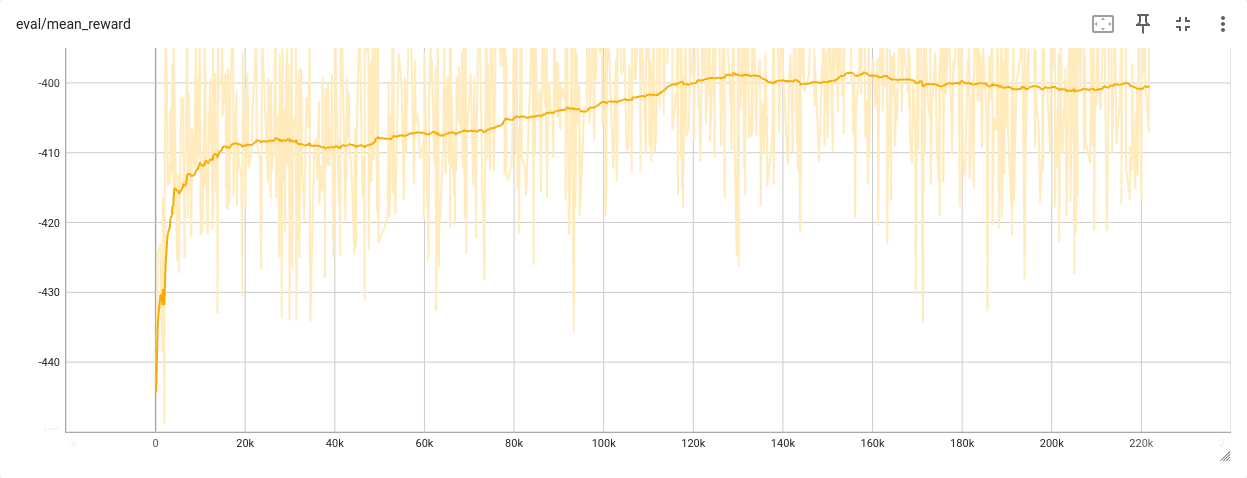
\includegraphics[scale=0.38]{../images/0089 PID Lernen.png}{\\Mittlerere Belohnung als Funktion der Episode aufgezeichnet und dargestellt mit Tensorboard. Wichtig ist das der Lernerfolg einsetzte nachdem die Belohnungsfunktion von der in \ref{Belohnung} abgewandelt wurde auf eine der From $-|e_v|$. In jedem Quadcopterschritt wird die Belohnung berechnet wie mit den vorgestellten Belohnungsfunktion \ref{Belohnung} und auf die Episodenbelohnung addiert, sodass nicht nur der Quadcopterschritt die Belohnung determiniert. Ob die veränderten Hyperparameter dieses Modell halbwegs akzeptabel lernen lassen haben oder tatsächlich die Belohnungsfunktion muss noch analysiert werden.}
\end{center}
\pagebreak 
Die Bilder zeigen exemplarisch, simulierte Positions-, Geschwindigkeits- und Drehlagetrajektorien in blau sowie Positions- und Geschwindigkeitssolltrajektorien in grün. Zunächst werden die Default PID-Parameter aus \ref{simcon:simcon} betrachtet.
\begin{center}
	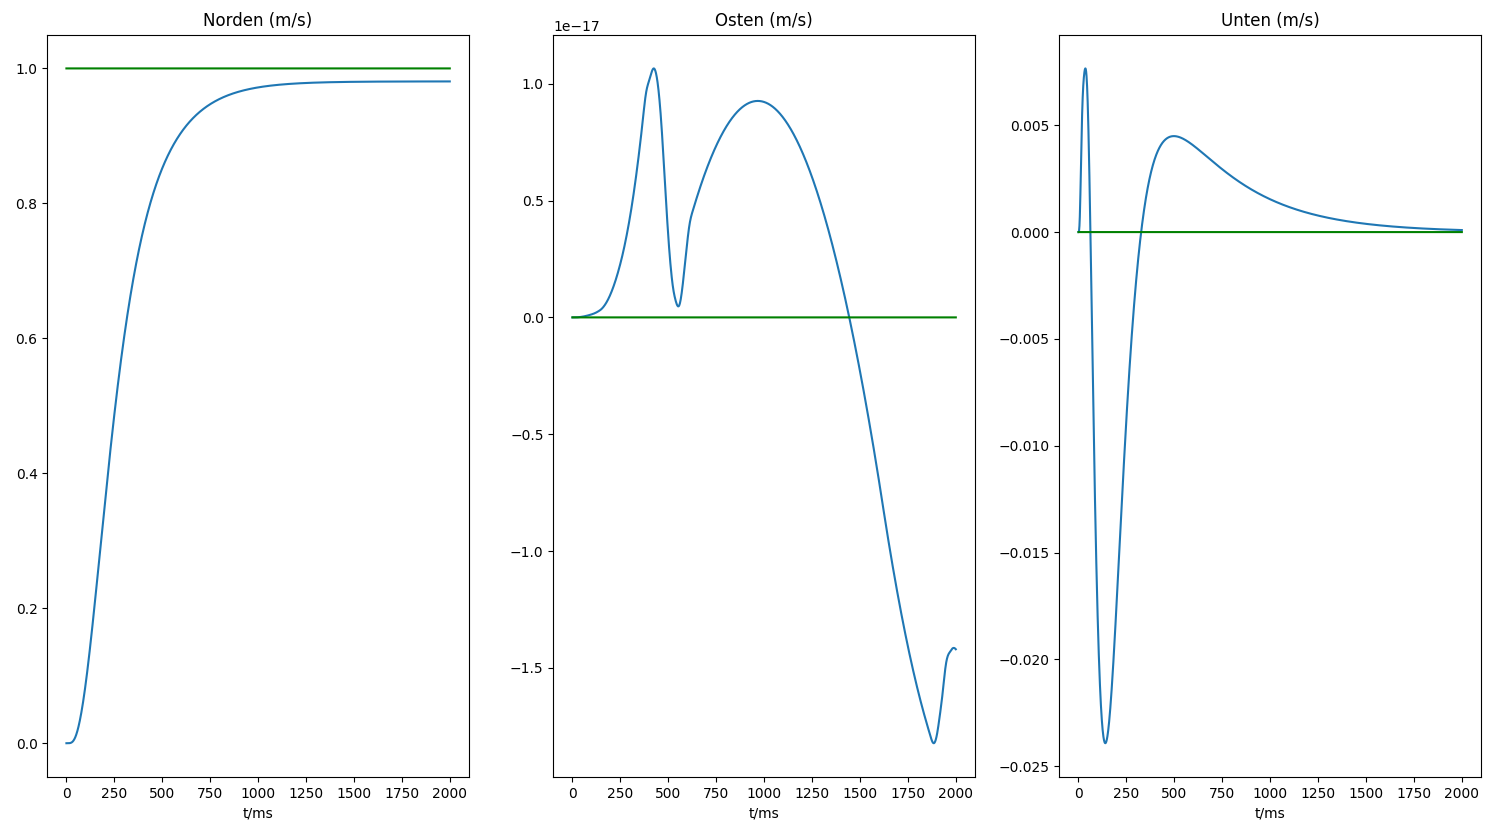
\includegraphics[scale=0.25]{../images/0096 Geschwindigkeit.png}{\\Die Istgeschwindigkeit folgt der Sollgeschwindigkeit in erster Näherung perfekt bis auf den unerwarteten verbleibenden Fehler auf der Nord-Dimension.}
\end{center}
\begin{center}
	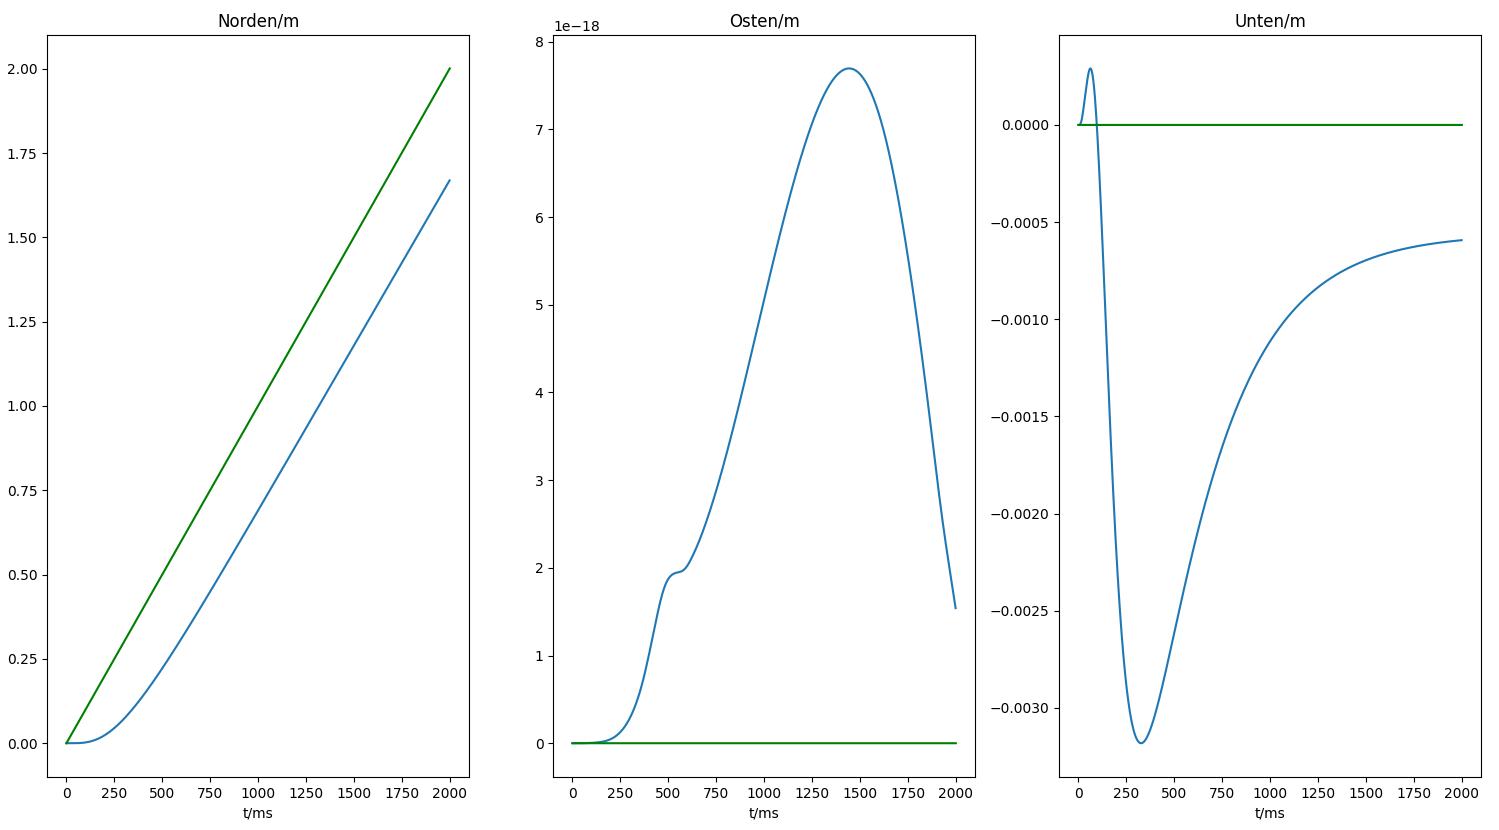
\includegraphics[scale=0.25]{../images/0098 Position.png}{\\Die Wirkung des verbleibenden Fehlers zwischen Ist- und Sollgeschwindigkeit ist im Positionsplot kaum sichbar da während der Beschleunigungsphase ein Offset entsteht.}
\end{center}
\begin{center}
	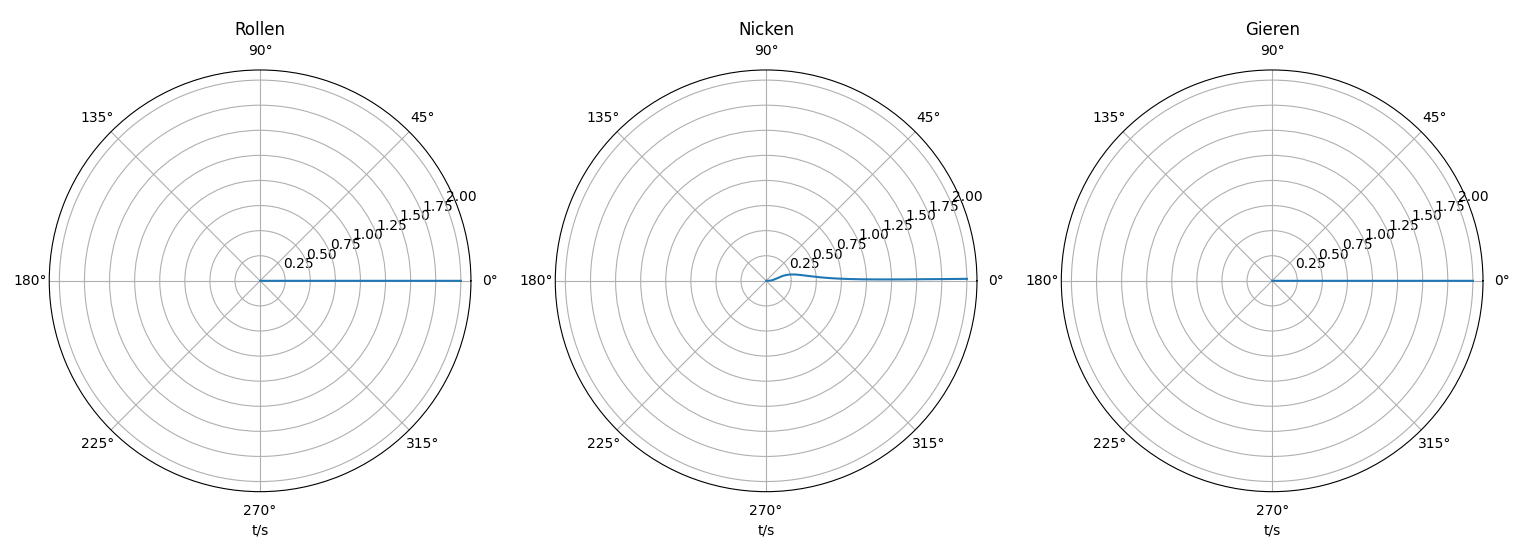
\includegraphics[scale=0.25]{../images/0097 Drehlage.png}{\\Winkel}
\end{center}
\pagebreak
Die Trajektorien ergeben sich wenn der PID-Regler mit gelernten Parametern arbeitet.
\begin{center}
	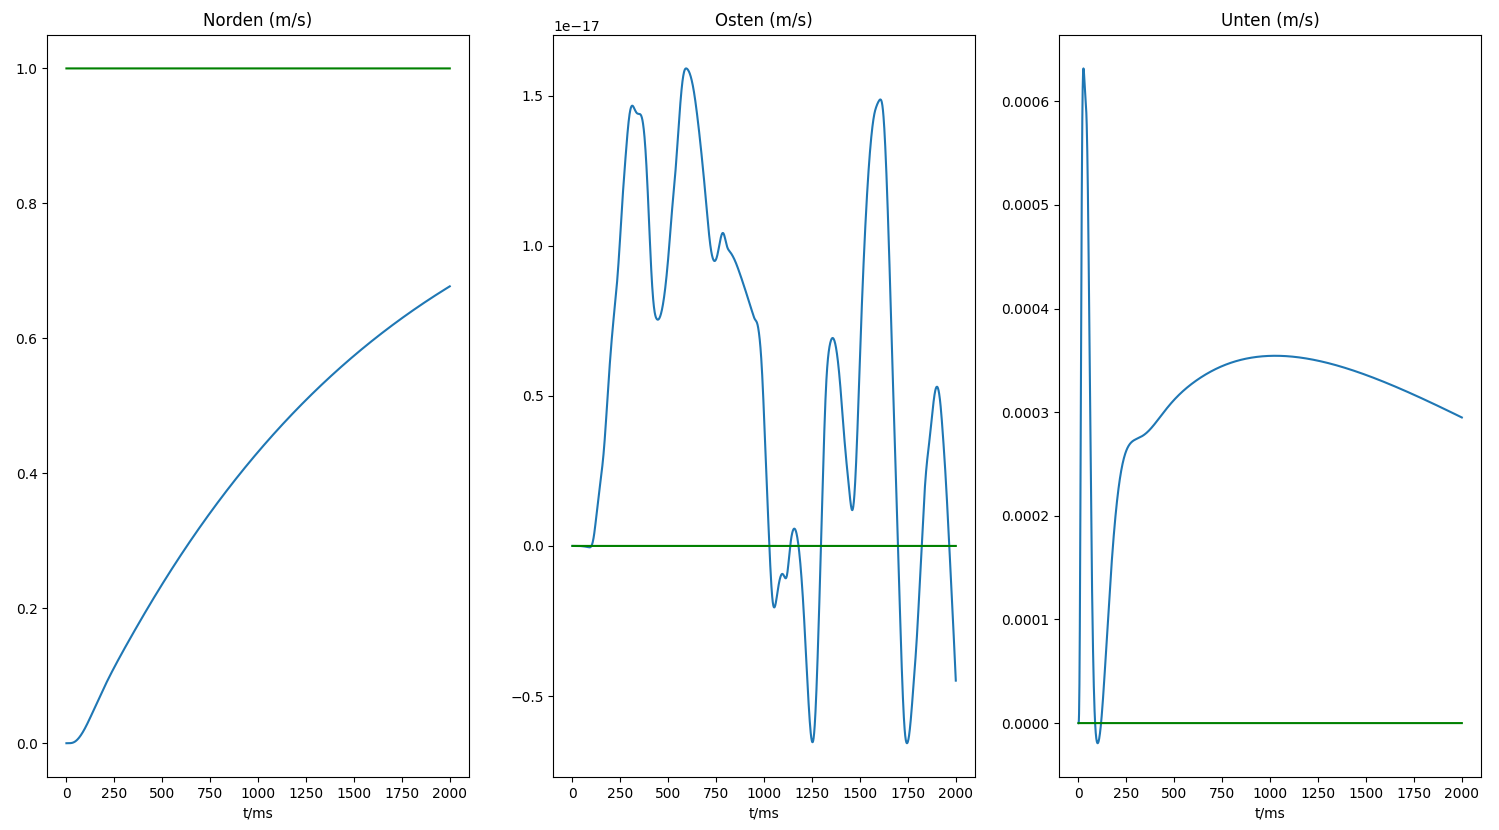
\includegraphics[scale=0.25]{../images/0093 Geschwindigkeit.png}{\\Die Parameter wurden gelernt sodass, der Regler gegen die Sollgeschwindigkeit konvergiert. Allerdings ist der gelernte PID-Regler grob abgeschätzt um den Faktor 4 mal später bei der halben Sollgeschwindigkeit.}
\end{center}
\begin{center}
	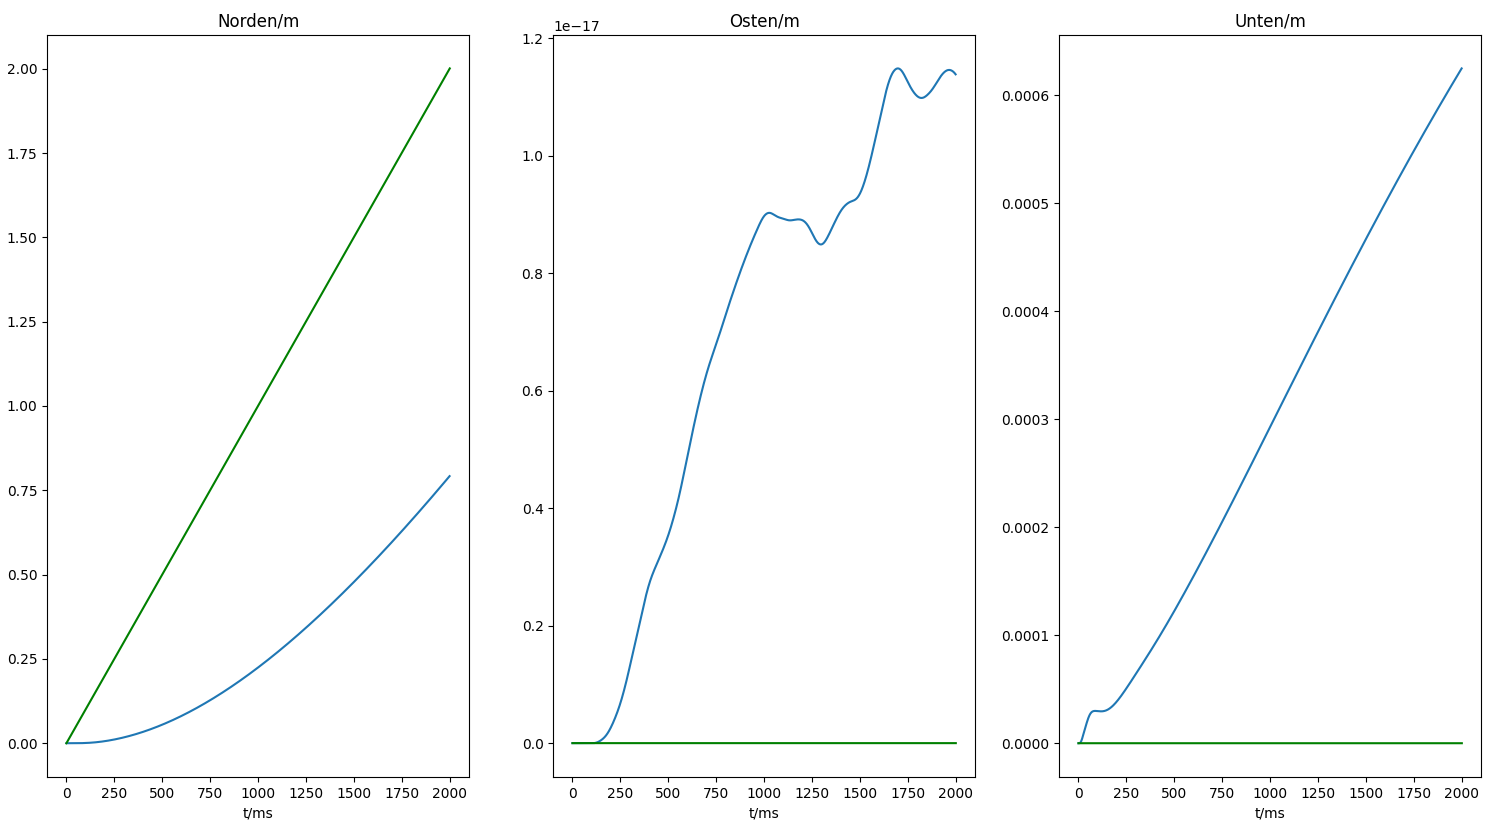
\includegraphics[scale=0.25]{../images/0094 Position.png}{\\Nach 2 Sekunden hat der Quadcopter noch keinen Meter zurückgelegt.}
\end{center}
\begin{center}
	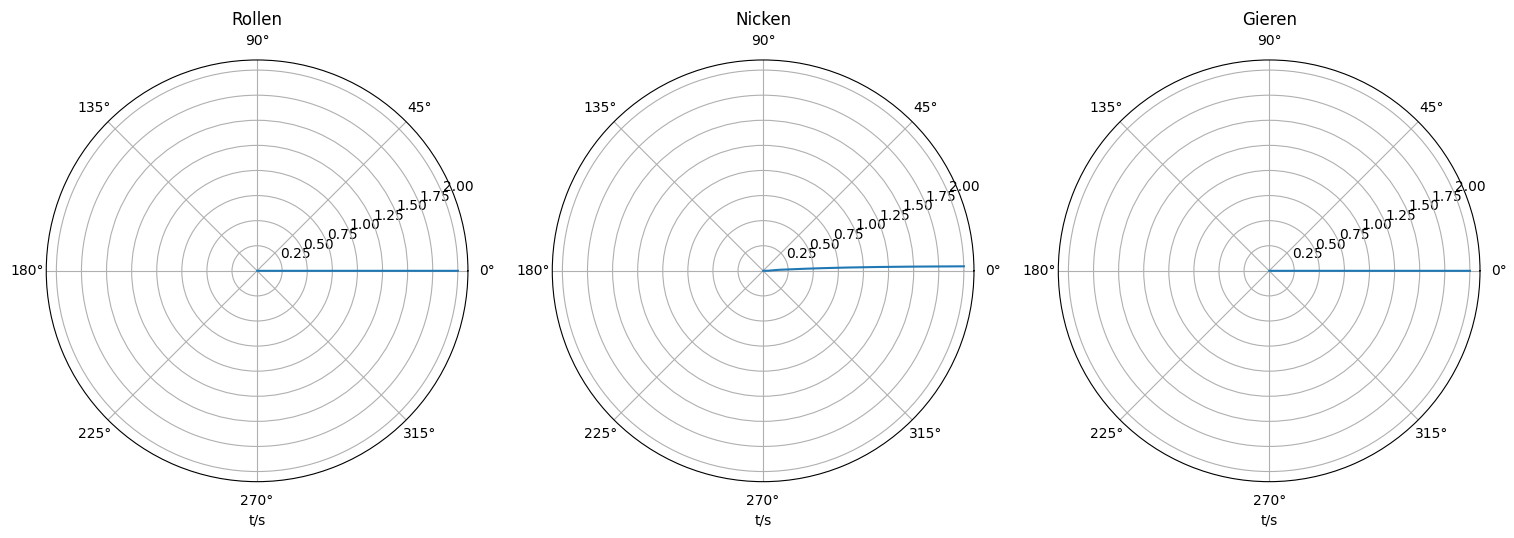
\includegraphics[scale=0.25]{../images/0095 Drehlage.png}{\\Der Quadcopter nickt deutlich schwächer.}
\end{center}
Die Herausforderung beim Lernen der PID-Parameter für den Geschwindigkeitsregler war Belohnungsfunktionen zu entwerfen die mit geringer Belohnungsvarianz und kontinuirlichen\\ Beobachtungs- und Aktionsräumen umgehen können. PID-Parameter Optimierung scheint ein stärker nichtkonvexes Problem zu sein als zunächst erwartet. Da nur einmal am Anfang pro Episode eine Aktion ausgeführt und eine Belohnung erfahren wird ist zudem die Sampleeffizient besonders gering. Die Kombination aus gewaltigem Quadcopterzustandsraum und Nichtlinearität verstärken den Fluch der Dimensionalität. Die Actor-Critic Architektur addressiert unter anderem das Problem der Sampleineffizienz scheint aber noch kein Allheilmittel zu sein. Grob geschätzt ist anzunehmen, dass nach einem Monat Training auf der vorliegenden Hardware alle Reglerparameter auf einen hohes Güteniveu gebracht werden können. Validieren lässt sich diese Aussage nur durch weiteres Training.

\subsection{\label{EndeZuEndeModell}Lernen des Ende-zu-Ende-Modells}
Ziel des Ende-zu-Ende-Lernens war mit PPO einen Agenten zu trainieren, welcher aus der Beobachtung bestimmter Quadcopterzustände direkt Motorbefehle vorhersagt, sodass die Quadcoptergeschwindigkeit so minimal wie möglich vom Geschwindigkeitssollvektor abweicht \ref{Geschwindigkeitssollvektor}. Der Aktionsraum besteht dementsprechend aus den vier Motorbefehlen.
\begin{align}
a_t &= 
\begin{pmatrix}
	u_{M1}\\
	u_{M2}\\
	u_{M3}\\
	u_{M4}
\end{pmatrix}
\end{align}
In \ref{link:ReinforcementLearningQuadcopter} wird auf ähnliche Weise versucht ein gleichwertiges Ziel zu erreichen.\\
Die Architektur für das Lernen des Ende-zu-Ende-Modells reduziert sich im Vergleich zur PID-Architektur auf das Umweltmodell, das Sollwertinterface, die Belohnungsfunktion und den Algorithmus des verstärkenden Lernens. Das Umweltmodell unterscheidet sich nur an den Schnittstellen zu dem aus der PID-Implementierung. Als Algorithmus wurde erneut Proximal-Policy-Optimization angewendet.
\begin{center}
\begin{tikzpicture}[
font=\sffamily, every label/.append style={font=\small\sffamily, align=center}]
\node[doc] (PPO) {PPO};

\node[below right=2cm of PPO, doc] (Umweltmodell) {Umweltmodell, $f_U$};

\node[above=1cm of PPO, doc] (Belohnungsfunktion) {Belohnungsfunktion};

\node[left=2cm of Belohnungsfunktion, doc] (Sollwertinterface) {Sollwertinterface};

\draw[-latex] (Umweltmodell) |- (PPO) node[right, midway, font=\small\sffamily]{$s_{t}$};

\draw[-latex] (Umweltmodell) |- (Belohnungsfunktion);

\draw[-latex] (Belohnungsfunktion) -- (PPO) node[right, midway, font=\small\sffamily]{$r_{t}$};

\draw[-latex] (Sollwertinterface) -- (Belohnungsfunktion) node[midway, above, font=\small\sffamily]{$s_{Soll}$};

\draw[-latex] (Sollwertinterface) |- (PPO) node[midway, left, font=\small\sffamily]{$s_{Soll}$};

\draw[-latex] (PPO) |- (Umweltmodell) node[left, midway, font=\small\sffamily]{$a_{t}$};

\node[
draw,
dashed,
rounded corners,
fit=(Regler) (Umweltmodell) (Sollwertinterface) (PPO) (Belohnungsfunktion),
inner sep=10pt,
label={above:{Architektur}}
](all2){};

\draw[-latex] (1.8, -0.2) arc (90:380:0.8) node[above, font=\small\sffamily]{$f_{PPO}$};

\end{tikzpicture}
\end{center}
Nach über 3e7 Episoden zeigte der Algorithmus keine Anzeichen von Belohnungsgewinnen und auch Änderungen der Hyperparameter zeigten keine signifikante Wirkung. Aus diesem Grund wurde eine Adaption der Architektur vorgenommen. Eine potenzielle Fehlerquelle für die Performance ist, dass das Modell sehr viele Zustände durchläuft und aus diesem Grund überfordert ist. Die extrem hohe Zustandsmenge des Problems hat insbesondere zwei Ursachen. Zunächst sind der Zustands- und Aktionsraum kontinuierlich da float32 Werte beide Räume bilden. Und zum anderen entspricht ein PPO-Sample einem Zeitschritt, weil die PPO-Updatefrequenz $f_{PPO}$ gleich der Umweltfrequenz $f_U$ ist. Statt als Frequenz kann man sich auch die Schritten $\Delta t_{PPO}$ und $\Delta t_{Modell}$ vorstellen. Das bedeutet, bei einer Schrittweite von 0.001s welche sinnvoll ist um das Umweltmodell präzise zu halten agiert das Modell 1000-mal pro Sekunde. Bei einer so hohen Anzahl an Aktionen ist es denkbar, dass das Modell zu Beginn, wenn die Strategiefunktion zufällige Aktionen produziert nicht lernen kann, da die Wirkung einer Aktion durch die Quadcopterdynamik bedingt erst deutlich später auftritt. Zu dem Zeitpunkt sind bereits sehr viele weitere Aktionen wirksam geworden, welche sich alle in ihrer Wirkung überlagern können. Deshalb ist bei zufälligen Aktionen denkbar, dass sich nur schwer oder gar nicht eine Aktion-Reaktion Beziehung lernen lässt, welche notwendig ist damit, dass Modell versteht welche Wirkung die eigenen Aktionen haben. Nun liegt es nahe testweise die PPO-Frequenz, um ein Vielfaches zu verringern. Gewählt wurde ein anderer Ansatz, welcher das Problem der optimalen Schrittperiodenwahl dem Modell selbst überlässt. Dazu hat das Modell neben dem Rotordrehraten noch eine Schrittperiodenaktion bekommen.
\begin{align}
a_t &= 
\begin{pmatrix}
	u_{M1}\\
	u_{M2}\\
	u_{M3}\\
	u_{M4}\\
	\frac{1}{f_{PPO}}
\end{pmatrix}
= \begin{pmatrix}
	u_{M1}\\
	u_{M2}\\
	u_{M3}\\
	u_{M4}\\
	\Delta t_{PPO}
\end{pmatrix},\ \text{mit}\ n\in N
\end{align}
Dadurch wird das Modell in die Lage versetzt die eigene Schrittweite $f_{PPO}$ im Verhältnis zur Umweltmodellschrittweite $f_U$ zu regulieren.
\begin{center}
\begin{tikzpicture}[font=\sffamily, every label/.append style={font=\small\sffamily, align=center}]
\node[doc] (PPO) {PPO};

\node[below right=2cm of PPO, doc] (Umweltmodell) {Umweltmodell, $f_U$};

\node[above=1cm of PPO, doc] (Belohnungsfunktion) {Belohnungsfunktion};

\node[left=2cm of Belohnungsfunktion, doc] (Sollwertinterface) {Sollwertinterface};

\draw[-latex] (Umweltmodell) |- (PPO) node[right, midway, font=\small\sffamily]{$s_{t}$};

\draw[-latex] (Umweltmodell) |- (Belohnungsfunktion);

\draw[-latex] (Belohnungsfunktion) -- (PPO) node[right, midway, font=\small\sffamily]{$r_{t}$};

\draw[-latex] (Sollwertinterface) -- (Belohnungsfunktion) node[midway, above, font=\small\sffamily]{$s_{Soll}$};

\draw[-latex] (Sollwertinterface) |- (PPO) node[midway, left, font=\small\sffamily]{$s_{Soll}$};

\draw[-latex] (PPO) |- (Umweltmodell) node[left, midway, font=\small\sffamily]{$a_{t}$};

\node[
draw,
dashed,
rounded corners,
fit=(Regler) (Umweltmodell) (Sollwertinterface) (PPO) (Belohnungsfunktion),
inner sep=10pt,
label={above:{Architektur}}
](all2){};

\draw[-latex] (1.8, -0.2) arc (90:380:0.8) node[above, font=\small\sffamily]{$f_{PPO}(a_t)$};

\draw[-latex] (PPO) to[out=270, in=180] (1, -1);
		
\end{tikzpicture}
\end{center}
Das neue Setup führt zu einer leicht adaptierten \textit{config.py} Datei. Auch mit dem neuen Ansatz war neben dem Aktionsraum und den Netzwerktopologien insbesondere die Lernrate Gegenstand zahlreicher Trainingstests.
\vspace*{0.5cm}
\begin{center}
\begin{tabular}[h]{|c|c|c|c|}
\hline 
Konfigurationsparameter & Wert \\
\hline 
Umweltparameter & \\
Schrittweite $\Delta t_{Modell}$ & 0.001s \\
Episodenende & 1s (1000 Schritte)\\
\hline
Quadtrain & \\
Ordnername & QM-16-08-24-EIPC55-E\\
$\alpha$ & 1e-4\\
Parallele Umwelten & 4\\
Batch & 16\\
Netzwerktopologie $\pi$ & [2, 2]\\
Netzwerktopologie $V^{\pi}$ & [2, 2]\\
\hline
Quadendezuende & \\
Aktionsraum & [100$\frac{rad}{s}$\ bis\ 600$\frac{rad}{s}$, 15$\Delta t_{Modell}$\ bis\ 45$\Delta t_{Modell}$]\\
Belohnungsfunktion & [$\alpha_r$ = 0.0, $\beta_r$ = 0.6, $\gamma_r$ = 0.2, $\delta_r$ = 0.2]\\
\hline
\end{tabular}
\end{center}
Mit dem neuen Setup konnte ein erstes Modell dazu gebracht werden zu lernen.
\begin{center}
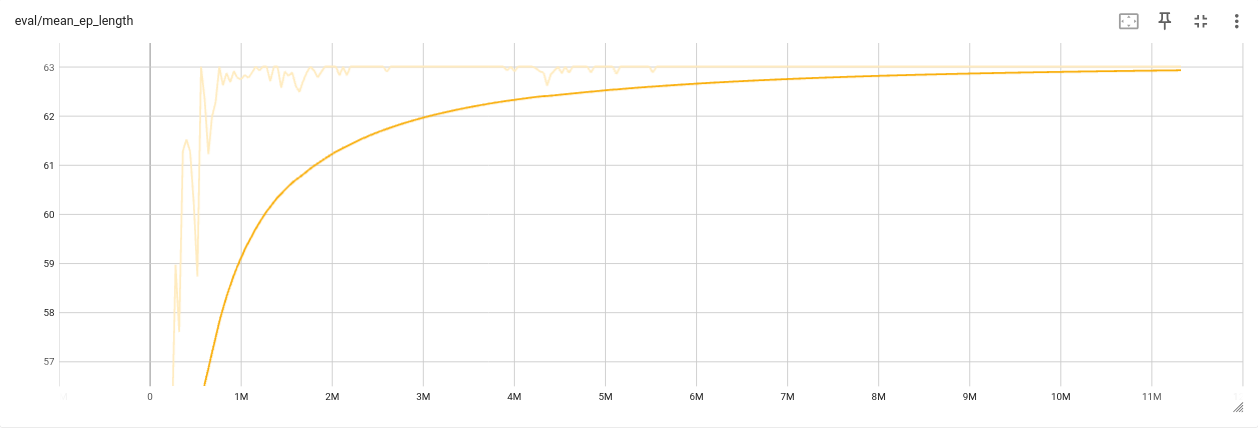
\includegraphics[scale=0.36]{../images/0091 Ende-zu-Ende 1.png}{\\Die mittlere Episodendauer nimmt ab. Das Modell scheint kürzere Updateschrittweiten zu bevorzugen. Welche darüberhinausgehende Bedeutung das Verhalten hat, könnte durch weiterführende Untersuchungen analysiert werden.}
\end{center}
\begin{center}
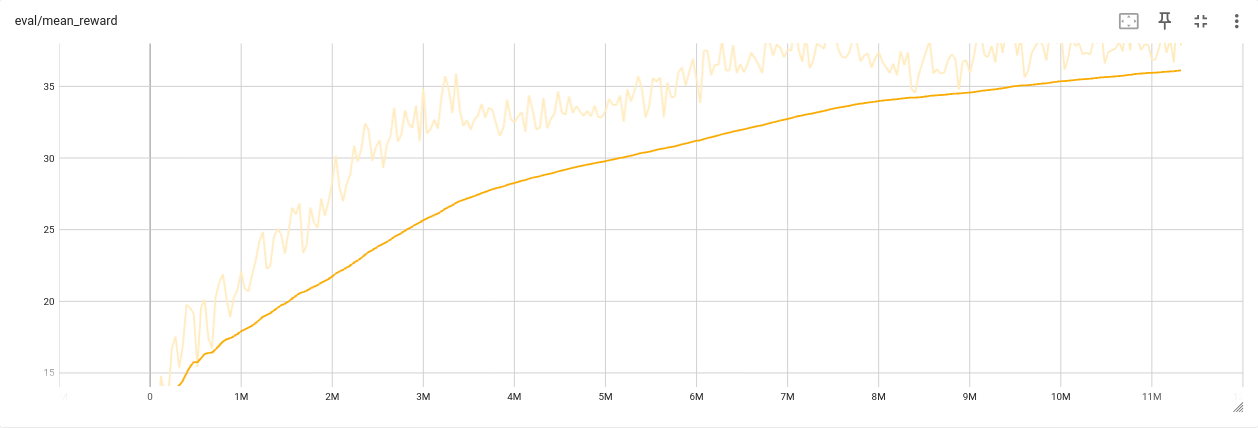
\includegraphics[scale=0.36]{../images/0092 Ende-zu-Ende 2.png}{\\Der Plot zeigt die erste stetig steigende Belohnungskurve eines Ende-zu-Ende-Modells. Ideal wäre, das die mittlere Belohnung der mittleren Episodenlänge entspricht. Doch davon ist das Modell nach 11.2e6 Episoden noch weit entfernt.}
\end{center}
Parallel zum Training mit modellbestimmter Schrittweite wurden die Hyperparameter der Default Ende-zu-Ende Version täglich aktualisiert und neue Modelle antrainiert. Mit folgenden Hyperparametern gelang es ein Modell zu trainieren welches lernte und akzeptabel performte.
\vspace*{0.5cm}
\begin{center}
\begin{tabular}[h]{|c|c|c|c|}
\hline 
Konfigurationsparameter & Wert \\
\hline 
Umweltparameter & \\
Schrittweite $\Delta t_{Modell}$ & 0.001s \\
Episodenende & 1s (1000 Schritte)\\
\hline
Quadtrain & \\
$\alpha$ & 1e-4\\
Parallele Umwelten & 4\\
Batch & 16\\
Netzwerktopologie $\pi$ & [2, 2]\\
Netzwerktopologie $V^{\pi}$ & [2, 2]\\
\hline
Quadendezuende & \\
Aktionsraum & [100$\frac{rad}{s}$\ bis\ 600$\frac{rad}{s}$, $\Delta t_{PPO}$ = $\Delta t_{Modell}$]\\
Belohnungsfunktion & [$\alpha_r$ = 0.0, $\beta_r$ = 0.6, $\gamma_r$ = 0.2, $\delta_r$ = 0.2]\\
\hline
\end{tabular}
\end{center}
\vspace*{0.5cm}
Als Regler kann dieses Modell noch nicht eingesetzt werden, da es insbesondere die Drehlageregelung\\ noch nicht generalisiert hat. Aber zumindest hat das Modell verstanden den 8 Sollgeschwindigkeitsvektoren mehr oder minder zu folgen. Zu erwarten ist, dass durch längeres Training die Güte weiter maximiert werden kann. Ob das tatsächlich der Fall ist, wird Gegenstand zukünftiger Trainings- und Testepochen sein.
\begin{center}
	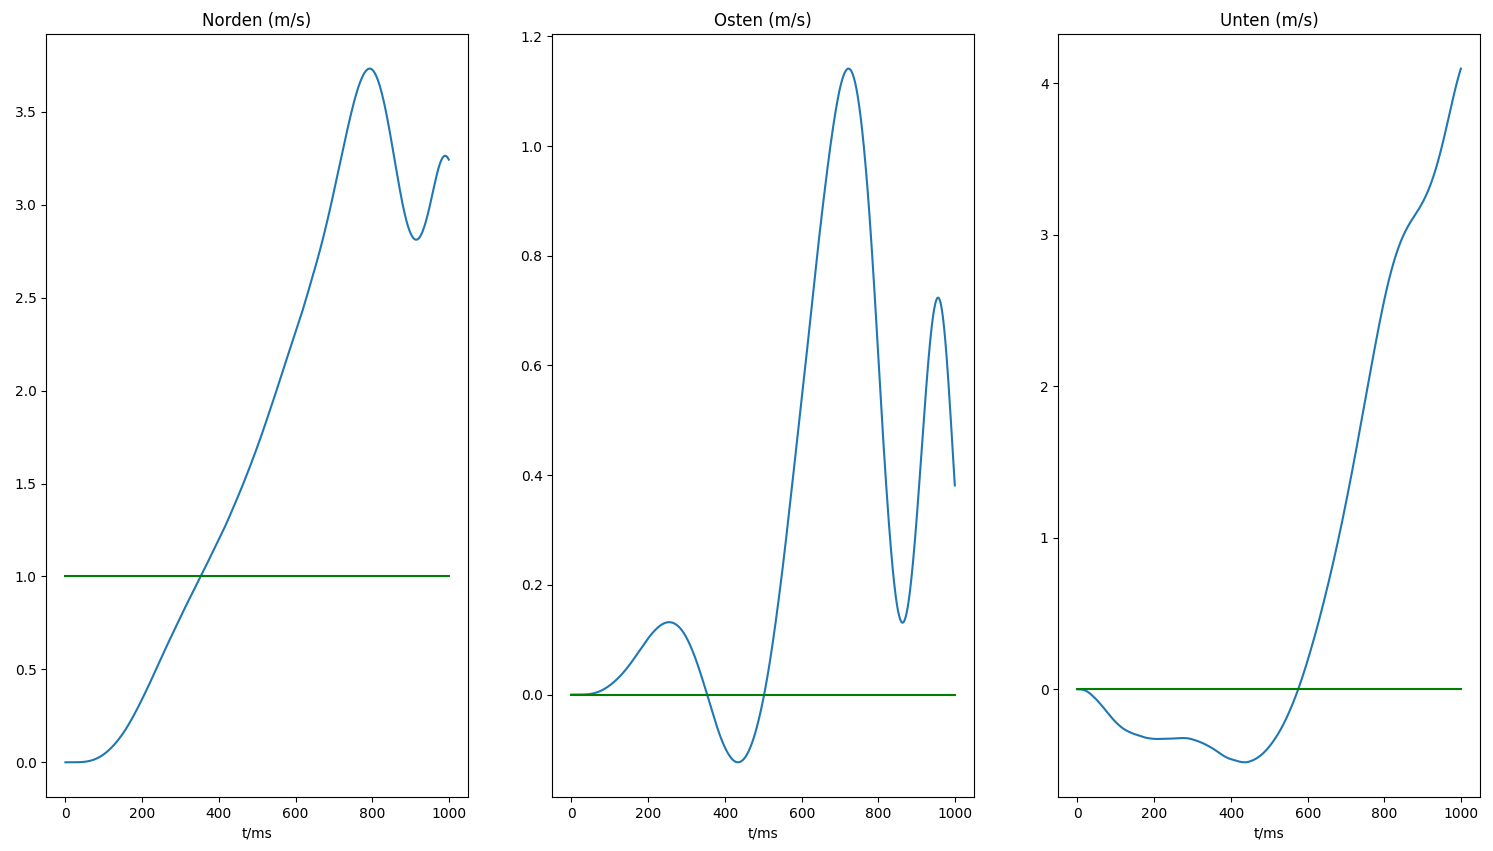
\includegraphics[scale=0.25]{../images/0081 Model E 1.png}{\\Sollgeschwindigkeit nach Norden ist 1 und nach Osten Null. Das Modell regelt den Quadcopter in die korrekte Richtung schwingt aber stark über. Auf den anderen Achsen zeigt das Modell unerwünschtes Verhalten, so driftet der Quadcopter um bis zu 1m und fällt 4m kann sich nach Osten hin aber stabilisieren mit einem erkennbar abnehmenden Fehler.}
\end{center}
\begin{center}
	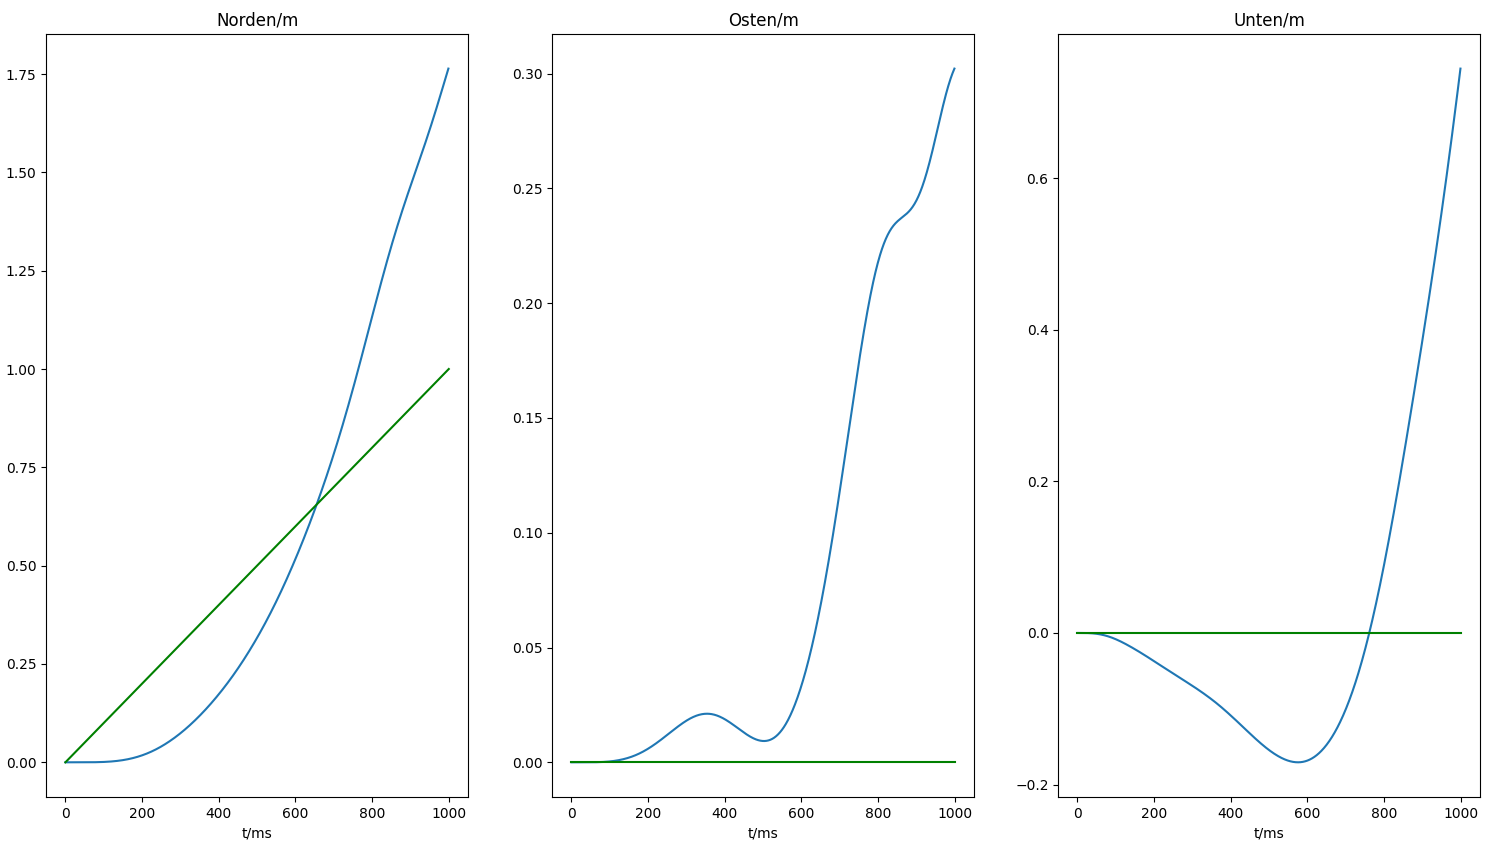
\includegraphics[scale=0.25]{../images/0080 Model E 2.png}{\\Interessant ist zunächst, dass das Integral zwischen der Differenz von der Soll- und Isttrajektorie über den Episodezeitraum von 1s ungefähr Null ist. Womöglich nur Zufall.}
\end{center}
\begin{center}
	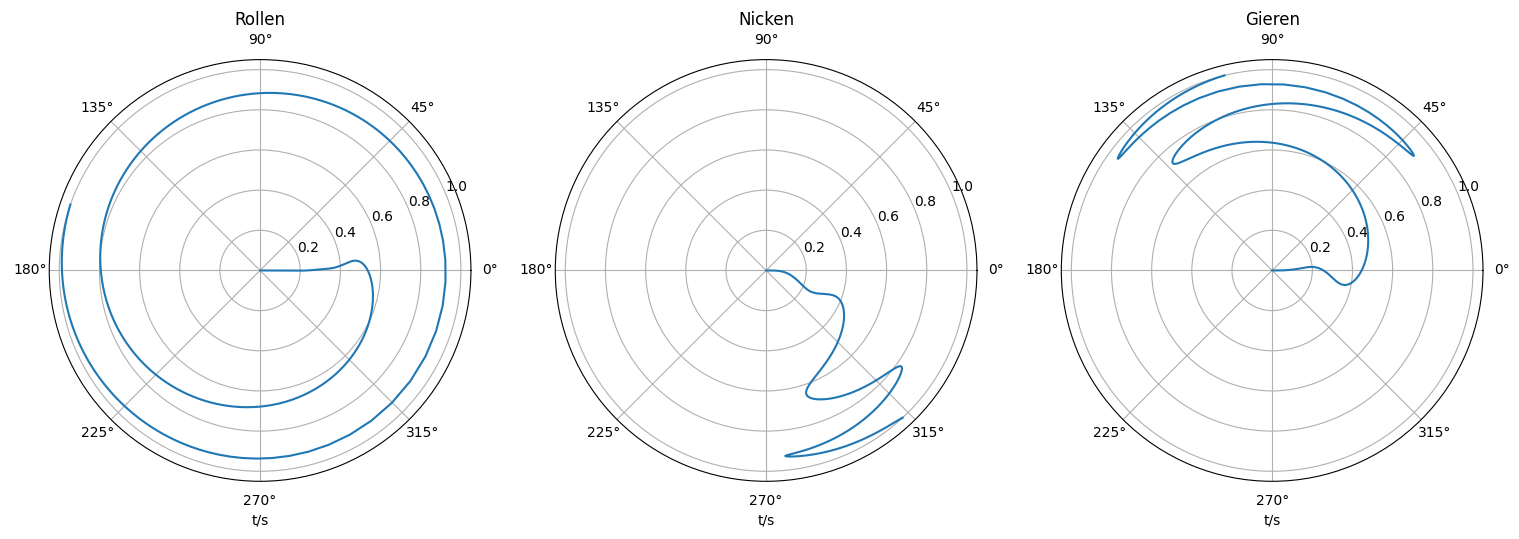
\includegraphics[scale=0.25]{../images/0079 Model E 3.png}{\\Die Drehlagentrajektorien offenbaren das Problem des Ende-zu-Ende-Modells. Nach circa 0.4s verliert es die Kontrolle über die Drehlage.}
\end{center}
Für einen anderen Geschwindigkeitssollvektor welcher nach Süd-Osten zeigt ergeben sich die folgenden Bilder.
\begin{center}
	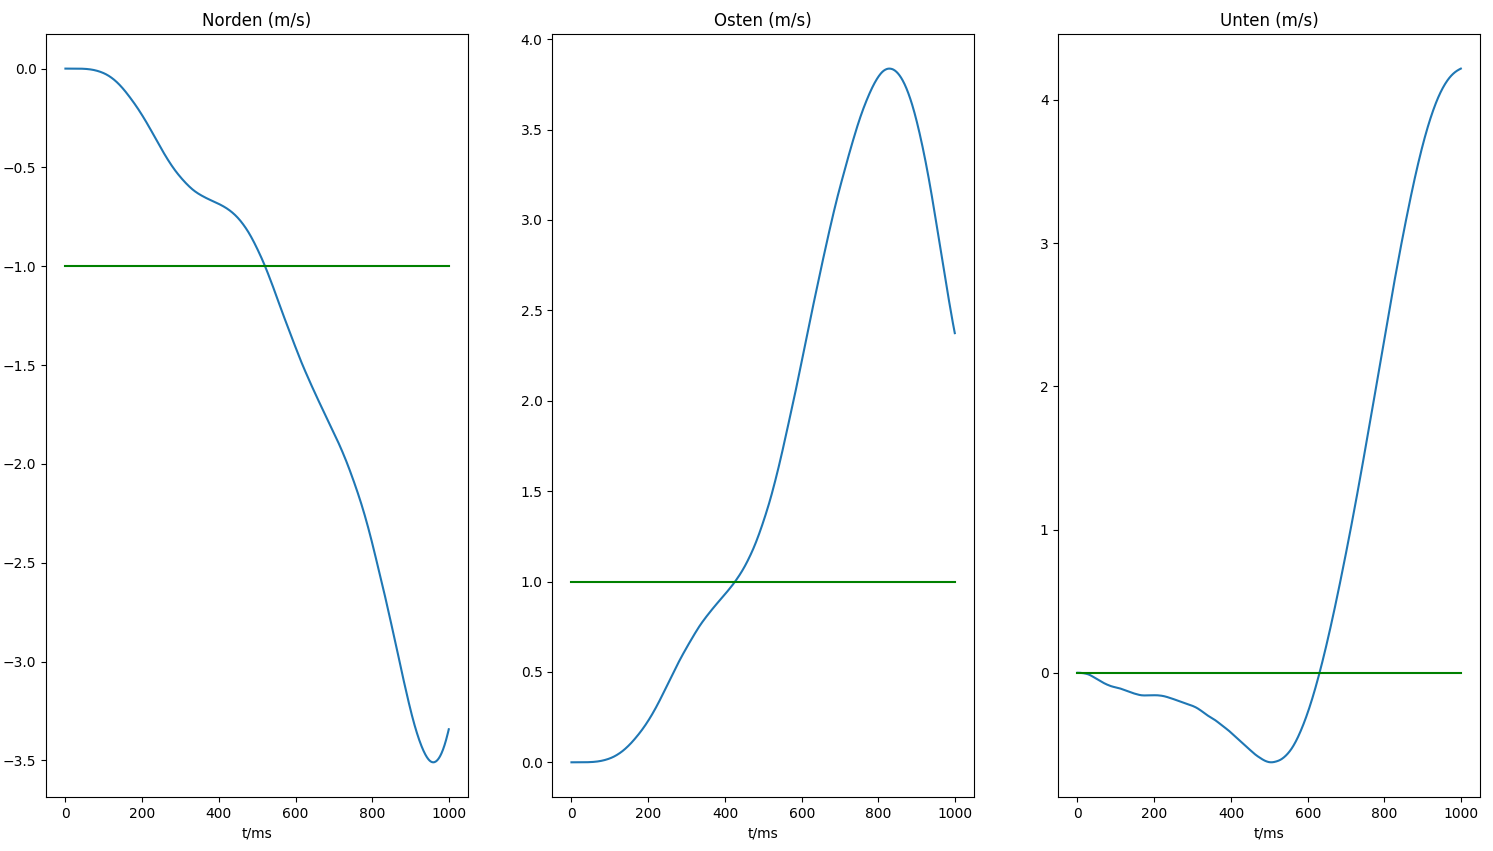
\includegraphics[scale=0.25]{../images/0085 Ende-zu-Ende Nordgeschwindigkeit Ostgeschwindigkeit Untengeschwindigkeit.png}{\\Grundsätzlich ist das Modell in der Lage grob den Sollgeschwindigkeiten zu folgen.}
\end{center}
\begin{center}
	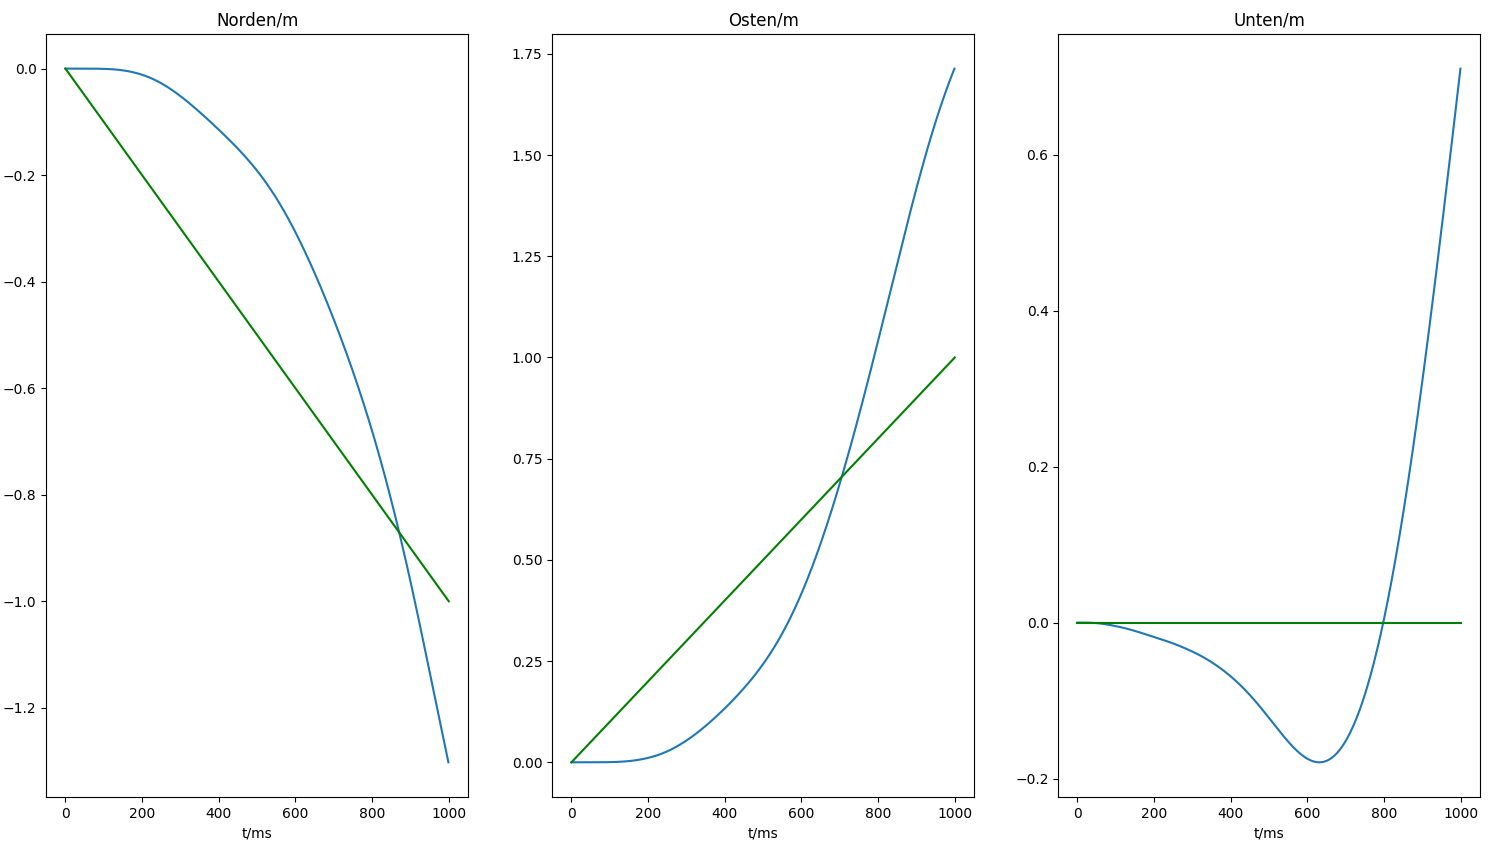
\includegraphics[scale=0.25]{../images/0084 Ende-zu-Ende Nord Ost Unten.png}{\\Die Positionstrajektorien zeigen ein ähnliches Bild wie im vorangegangen Beispiel.}
\end{center}
\begin{center}
	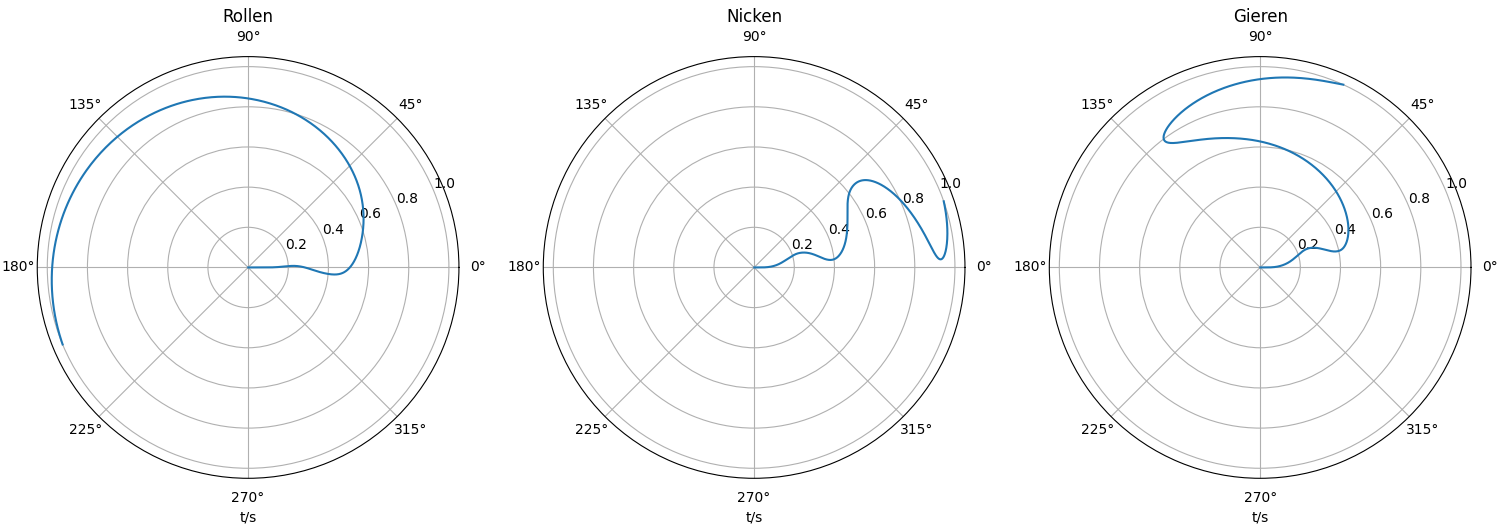
\includegraphics[scale=0.25]{../images/0086 Ende-zu-Ende Rolllage Nickrate Gierrate.png}{\\Auch bei einem anderen Sollgeschwindigkeitsvektor verliert das aktuell beste Modell die Kontrolle über den Quadcopter macht aber auch deutlich, das es die Aufgabe verstanden hat.}
\end{center}

\subsection{\label{Reglerimplementierung:Reglerimplementierung}Implementierung des Reglers}
Die Implementierung des Reglers umfasst alle Implementierungsschritte, die notwendig sind zur Quadcopterzustandsschätzung, zur Berechnung von Reglerbefehlen und für die BLDC-Motorenansteuerung.\\
Für die Programmierung der Informationsflussteilsysteme wurde neben der STM32CubeIDE Entwicklungsumgebung auch Zephyr in Kombination mit Visual Studio Code als Implementierung des Reg Entwicklungsumgebung betrachtet. Nachdem sich der Aufwand für das vollumfängliche Lernen des Zephyr-Devicetrees als zu umfänglich herausgestellt hatte, wurde für die weitere Entwicklung mit der STM32CubeIDE in der Version 1.16.0 gearbeitet.\\
Aus zeitlichen Gründen konnte eine Implementierung des trainierten Modells auf dem Mikrocontroller nicht angegangen geschweige den getestet werden. Dafür wurde der PID-Regler aus \ref{simcon:simcon} adaptiert und portiert auf den STM32F411RE Mikrocontroller. \\
Die vier BLDC-Motoren werden angesteuert über vier unabhängige PWM-Signale welche alle mit Timer 1 generiert werden. Die PWM-Signale liegen auf den Pins PA8, PA9, PA10, und PA11. Aus der Pinkonfiguration ist ersichtlich, dass diesen Pins jeweils ein Timer-Kanal zugeordnet ist. 
\begin{center}
	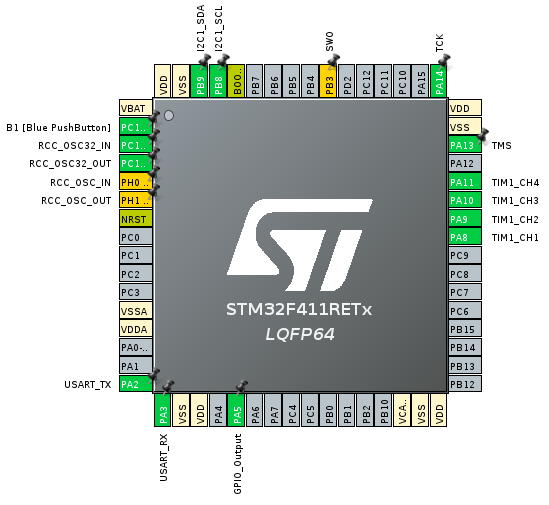
\includegraphics[scale=0.5]{../images/0064 Pinbelegung.png}{\\Pinkonfiguration in der STM32CubeIDE}
\end{center}
Das Pindiagramm wurde herangezogen um die Pins auf dem Board zu lokalisiert. Um die Pins während der Entwicklungsphase schnell zu finden wurden die verwendeten Pins vorsichtig angewinkelt.
\begin{center}
	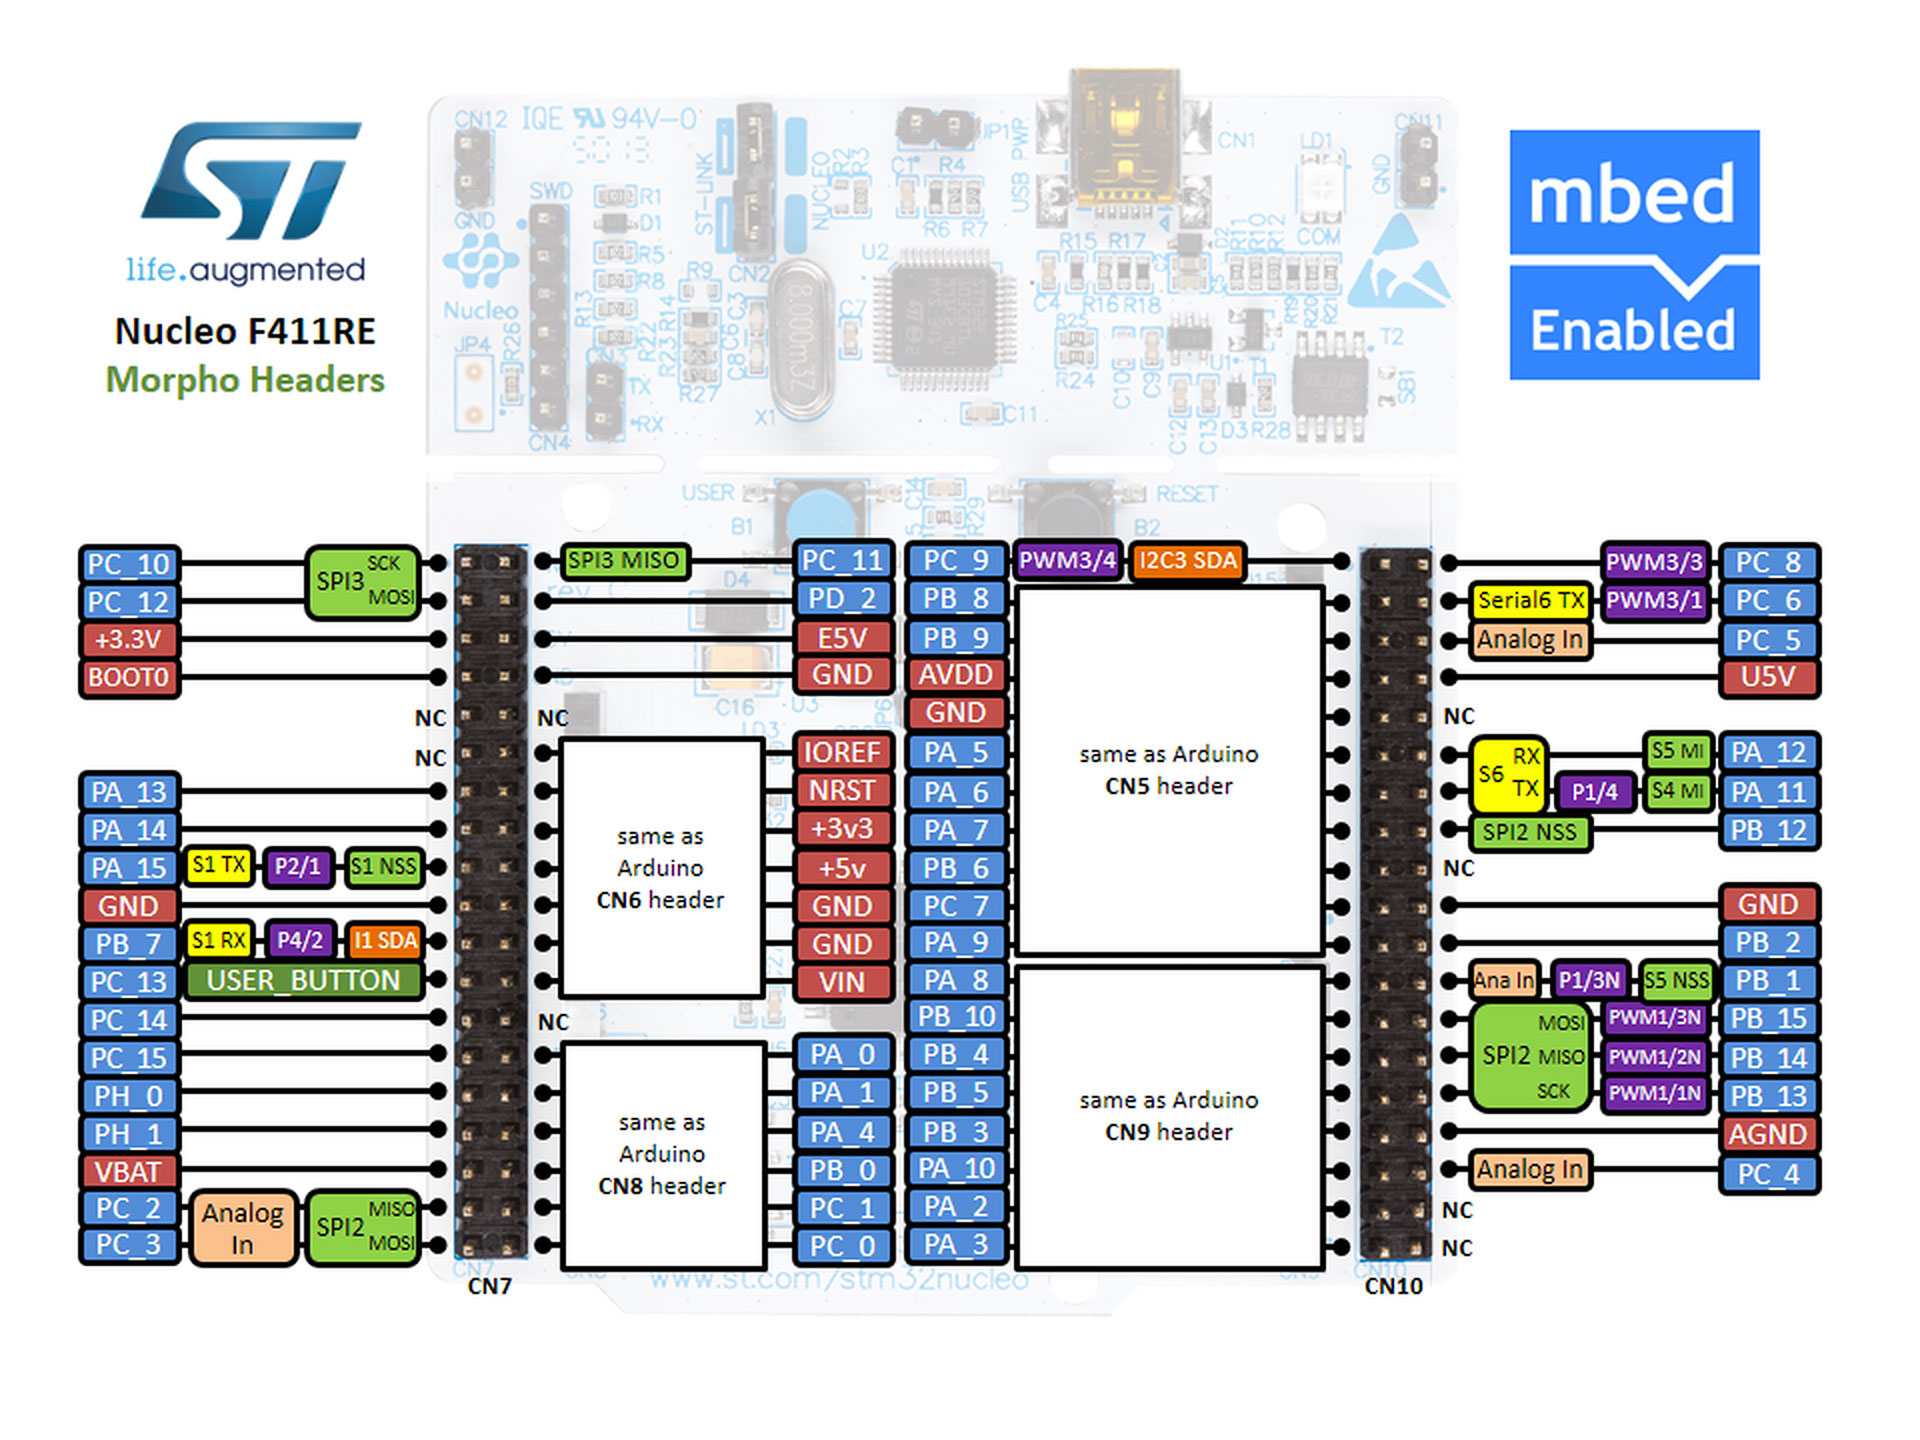
\includegraphics[scale=0.14]{../images/0067 Pinout NUCLEO F411RE.jpeg}{\\Pindiagramm des NUCLEO-F411RE Boards \ref{bild:Pinout}}
\end{center}
Der Duty-Cycle entspricht dem Wert im Capture-Compare-Register (CCR) in welche die Sollwerte direkt geschrieben werden. Die PWM-Frequenz mit welcher die Treiber arbeiten kann zwischen 50Hz und 60Hz liegen \ref{link:Treiberdatenblatt}. Diese wurde mit der System Clock eingestellt. Bei einer Frequenz von 16Mhz wurde ein Prescaler mit Wert 8 und einer Periode von 30259 eingestellt, um circa 60Hz für das PWM-Signal bereitzustellen.
\begin{center}
	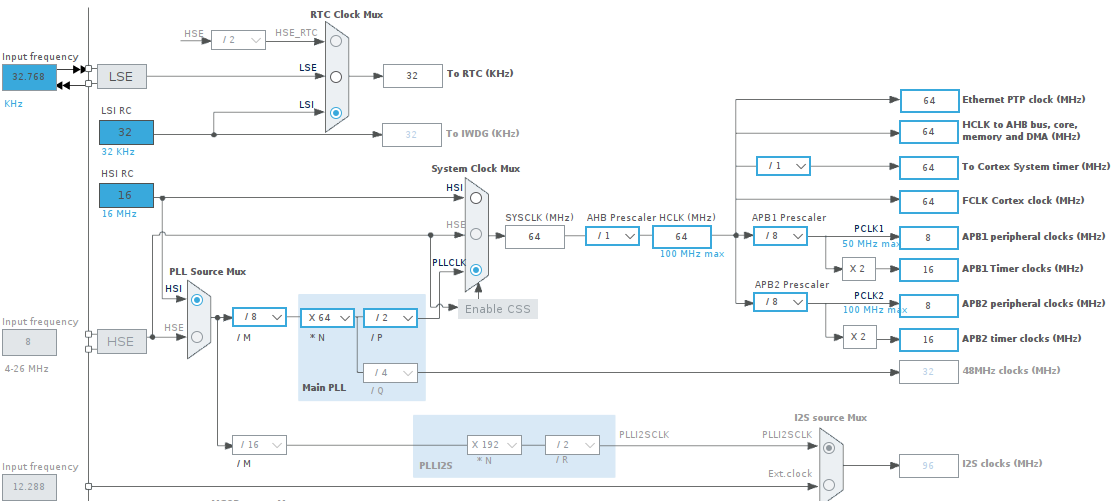
\includegraphics[scale=0.35]{../images/0065 Clock.png}{\\Clock Konfiguration in der STM32CubeIDE}
\end{center}
Mit einer Frequenz von 100Hz wird die Funktion \textit{regelschritt} ausgeführt. Frei wählbar war die Frequenz nicht da es galt sie auf die MotionFX Sensorfusion abzustimmen. Die Funktion \textit{MX\_MEMS\_INIT} initialisiert die Inertiale Messeinheit und konfigurert den Kalmanfilter für die Sensorfusion. 
\begin{center}
\begin{tikzpicture}[font=\sffamily,every label/.append
style={font=\small\sffamily,align=center}]

\node[doc, fill=white] (Quadcontroller) {quadregler.c\\  \begin{lstlisting}[language=C, basicstyle=\fontsize{8}{10}\selectfont]
...
int main(void)
{
	uint16_t timer_val;

	HAL_Init();
	SystemClock_Config();
	MX_GPIO_Init();
	MX_DMA_Init();
	MX_CRC_Init();
	MX_TIM3_Init();
	MX_RTC_Init();
	MX_TIM1_Init();
	MX_TIM2_Init();
	MX_MEMS_Init();
	MX_USART2_UART_Init();

	HAL_TIM_PWM_Start(&htim1, TIM_CHANNEL_1);
	HAL_TIM_PWM_Start(&htim1, TIM_CHANNEL_2);
	HAL_TIM_PWM_Start(&htim1, TIM_CHANNEL_3);
	HAL_TIM_PWM_Start(&htim1, TIM_CHANNEL_4);

	DWT_Start();
	HAL_TIM_Base_Start(&htim2);
	timer_val = __HAL_TIM_GET_COUNTER(&htim2);

	while (1)
	{
		if (__HAL_TIM_GET_COUNTER(&htim2) - timer_val >= 20)
		{
			timer_val = __HAL_TIM_GET_COUNTER(&htim2);
			regelschritt();
		}
	}
}
...
\end{lstlisting}
};
\end{tikzpicture}
\end{center}
Unter anderem wird in dem Prozess die Funktion \textit{MotionFX\_manager\_init} aufgerufen. In dieser kann unter anderem die Orientierung der Sensoren festgelegt werden. Hilfreich war dabei die Dokumention von STMicroelectronics, ganz besonders \ref{link:MotionFX}.
\begin{center}
\begin{tikzpicture}[font=\sffamily,every label/.append
style={font=\small\sffamily,align=center}]

\node[doc, fill=white] (Quadcontroller) {MotionFX\_manager\_init.c\\\begin{lstlisting}[language=C, basicstyle=\fontsize{8}{10}\selectfont]
...
void MotionFX_manager_init(void)
{
	...
	MotionFX_initialize((MFXState_t *) mfxstate);
	MotionFX_getKnobs(mfxstate, ipKnobs);

	ipKnobs->ATime = 1.0;
	ipKnobs->MTime = 8.0;
	ipKnobs->FrTime = 1.0;
	strcpy(ipKnobs->acc_orientation, "NED");
	strcpy(ipKnobs->gyro_orientation, "NED");
	strcpy(ipKnobs->mag_orientation, "NED");
	BSP_SENSOR_ACC_GetOrientation(ipKnobs->acc_orientation);
	BSP_SENSOR_GYR_GetOrientation(ipKnobs->gyro_orientation);
	BSP_SENSOR_MAG_GetOrientation(ipKnobs->mag_orientation);
	ipKnobs->gbias_acc_th_sc = GBIAS_ACC_TH_SC;
	ipKnobs->gbias_gyro_th_sc = GBIAS_GYRO_TH_SC;
	ipKnobs->gbias_mag_th_sc = GBIAS_MAG_TH_SC;
	ipKnobs->output_type = MFX_ENGINE_OUTPUT_NED;
	// Lernmodus
	ipKnobs->LMode = 1;
	...
}
...
\end{lstlisting}
};
\end{tikzpicture}
\end{center}
In der Funktion \textit{regelschritt} werden alle Tasks ausgeführt, welche der Regler hat. Zunächst werden die Sensoren auslesen und mit der Bibliothek MotionFX fusioniert.
\begin{center}
\begin{tikzpicture}[font=\sffamily,every label/.append
style={font=\small\sffamily,align=center}]

\node[doc, fill=white] (Quadcontroller) {quadcontroller.c\\\begin{lstlisting}[language=C, basicstyle=\fontsize{8}{10}\selectfont]
...
void regelschritt(void) {
	// Beschleunigungsensor auslesen mit einer Funktion
	// des X-Cube-MEMS1 Board Support Package
	// BSP_SENSOR_ACC_GetAxes(&AccValue);
	READ_ACCELEROMETER();
	// Gyro auslesen
	// BSP_SENSOR_GYR_GetAxes(&GyrValue);
	READ_GYRO();
	// Magnetometer auslesen
	// BSP_SENSOR_MAG_GetAxes(&MagValue);
	READ_MAG();
	/* Convert angular velocity from [mdeg/s] to [deg/s] */
	// Gieren (Uhrzeigersinn)
	data_in.gyro[0] = (float) GyrValue.x * FROM_MDPS_TO_DPS;
	// Nicken (Nase nach unten ist negatives nicken)
	data_in.gyro[1] = (float) GyrValue.y * FROM_MDPS_TO_DPS;
	// Rollen (Mit Blick von hinten im Uhrzeigersinn)
	data_in.gyro[2] = (float) GyrValue.z * FROM_MDPS_TO_DPS;
	// Norden in g
	data_in.acc[0] = (float) AccValue.x * FROM_MG_TO_G;
	// Osten in g
	data_in.acc[1] = (float) AccValue.y * FROM_MG_TO_G;
	// Oben in g
	data_in.acc[2] = (float) AccValue.z * FROM_MG_TO_G;
	data_in.mag[0] = (float) MagValue.x * FROM_MGAUSS_TO_UT50;
	data_in.mag[1] = (float) MagValue.y * FROM_MGAUSS_TO_UT50;
	data_in.mag[2] = (float) MagValue.z * FROM_MGAUSS_TO_UT50;
	delta_t_s = DWT_Stop() * 1e-6f;
	DWT_Start();
	// Sensorfusion bei 100Hz
	MotionFX_manager_run(fusionin, fusionout, 0.01f);
	...
}
...
\end{lstlisting}
};
\end{tikzpicture}
\end{center}
Eingangswerte für die Fusion wurden vorher in die Struktur \textit{fusionein} geschrieben und Ausgangswerte werden in \textit{fusionout} gespeichert. Diese sind die Lage in Quaternionenform und in Eulerwinkelform, lineare Beschleunigung, der Gravitationsvektor und ein Richtungsfehler. Daraufhin werden die Werte skaliert und zu Gleitkommazahlen umgewandelt, sodass Sie vom Drehlage- und geschwindigkeitsrechner sinnvoll prozessiert werden. Da die linearen Beschleunigungswerte für den Geschwindigkeitsregler einmal integriert werden wird $\Delta t_{PID}$ bestimmt. Auch möglich wäre mit einem Konstanten Wert von 1e-2s zu arbeiten da diese Frequenz im Regelfall vorliegt. Für den Entwicklungszeitraum hat die Messung als robuster erwiesen.
\begin{center}
\begin{tikzpicture}[font=\sffamily,every label/.append
style={font=\small\sffamily,align=center}]

\node[doc, fill=white] (Quadcontroller) {quadcontroller.c\\\begin{lstlisting}[language=C, basicstyle=\fontsize{8}{10}\selectfont]
...
void regelschritt(void) {
	...
	// Setzen der Sollposition mit Joystickwerten
	sollgeschwindigkeit.norden = joystick_nicken / 50.0f;
	sollgeschwindigkeit.osten = joystick_rollen / 50.0f;
	sollgeschwindigkeit.unten = joystick_schub / 50.0f;

	// Integration der Beschleunigungen
	// [m/s]
	geschwindigkeit[NORDEN] += (
		delta_t_s * fusionout->linear_acceleration[SENSOR_NORDEN] / 9.81f
	);
	// [m/s]
	geschwindigkeit[OSTEN] += (
		delta_t_s * fusionout->linear_acceleration[SENSOR_WESTEN] / 9.81f
	);
	// [m/s]
	geschwindigkeit[UNTEN] += (
		delta_t_s * fusionout->linear_acceleration[SENSOR_OBEN] / 9.81f
	);
	drehlage.w = fusionout->quaternion[QW];
	drehlage.x = fusionout->quaternion[QX];
	drehlage.y = fusionout->quaternion[QY];
	drehlage.z = fusionout->quaternion[QZ];
	// Rollwinkel [deg/s]
	drehrate.rollen = (fusionout->rotation[2] - drehlage_tminus1.rollen) / delta_t_s;
	// Nickwinkel [deg/s]
	drehrate.nicken = (fusionout->rotation[1] - drehlage_tminus1.nicken) / delta_t_s;
	// Gierwinkel [deg/s]
	drehrate.gieren = 0.0f * data_in.gyro[0];
	drehlage_tminus1.rollen = fusionout->rotation[2];
	drehlage_tminus1.nicken = fusionout->rotation[1];
	omega_dot.rollen = (drehrate.rollen - drehgeschwindigkeit_tminus1.rollen) / delta_t_s;
	omega_dot.nicken = (drehrate.nicken - drehgeschwindigkeit_tminus1.nicken) / delta_t_s;
	omega_dot.gieren = 0.0f;
	drehgeschwindigkeit_tminus1.rollen = drehrate.rollen;
	drehgeschwindigkeit_tminus1.nicken = drehrate.nicken;
	...
	// Drehlage- und -geschwindigkeitsregler
	...
	// Setzen der PWM-Signale 
	skalar = (pwmoberegrenze - pwmunteregrenze) / 1000.0f;
	// Pin PA8
	TIM1->CCR1 = (
		(
			skalar * schub * ((
				w_cmd[M1] + w_cmd_tminus1[M1]
			) / 2) + pwmunteregrenze
		) / 1000.0f
	) * 30259;
	...
}
...
\end{lstlisting}
};
\end{tikzpicture}
\end{center} 
Neben der Drehlage arbeitet der Geschwindigkeitsregler auch mit der Drehrate und optional der Drehbeschleunigung. Auf die Drehrate wird durch einen Differenzenquotienten der Drehlage, in Eulerwinkelform, geschlossen. Liegen alle Werte als Gleitkommazahlen vor und sind nicht undefiniert berechnet der Drehraten- und -geschwindigkeitsregler die Motorbefehle. Diese werden skaliert und mit einem einfachen Tiefpass beaufschlagt um die Elektronik und Mechanik zu schonen. Der Duty-Cycle muss auf die ganzzahlige Periode des Timers hoch multipliziert werden. Am Oszilloskop wurde die Validität aller Motorsignale geprüft, wofür die Testbench \ref{testbench:testbench} die perfekten Voraussetzungen bot.\\
Mit der Implementierung des Reglers auf dem Mikrocontroller war die Entwicklung aller System für den Quadcopter vorerst abgeschlossen. Das System war damit in einem Zustand der erste operationelle Tests erlaubte.
\begin{center}
	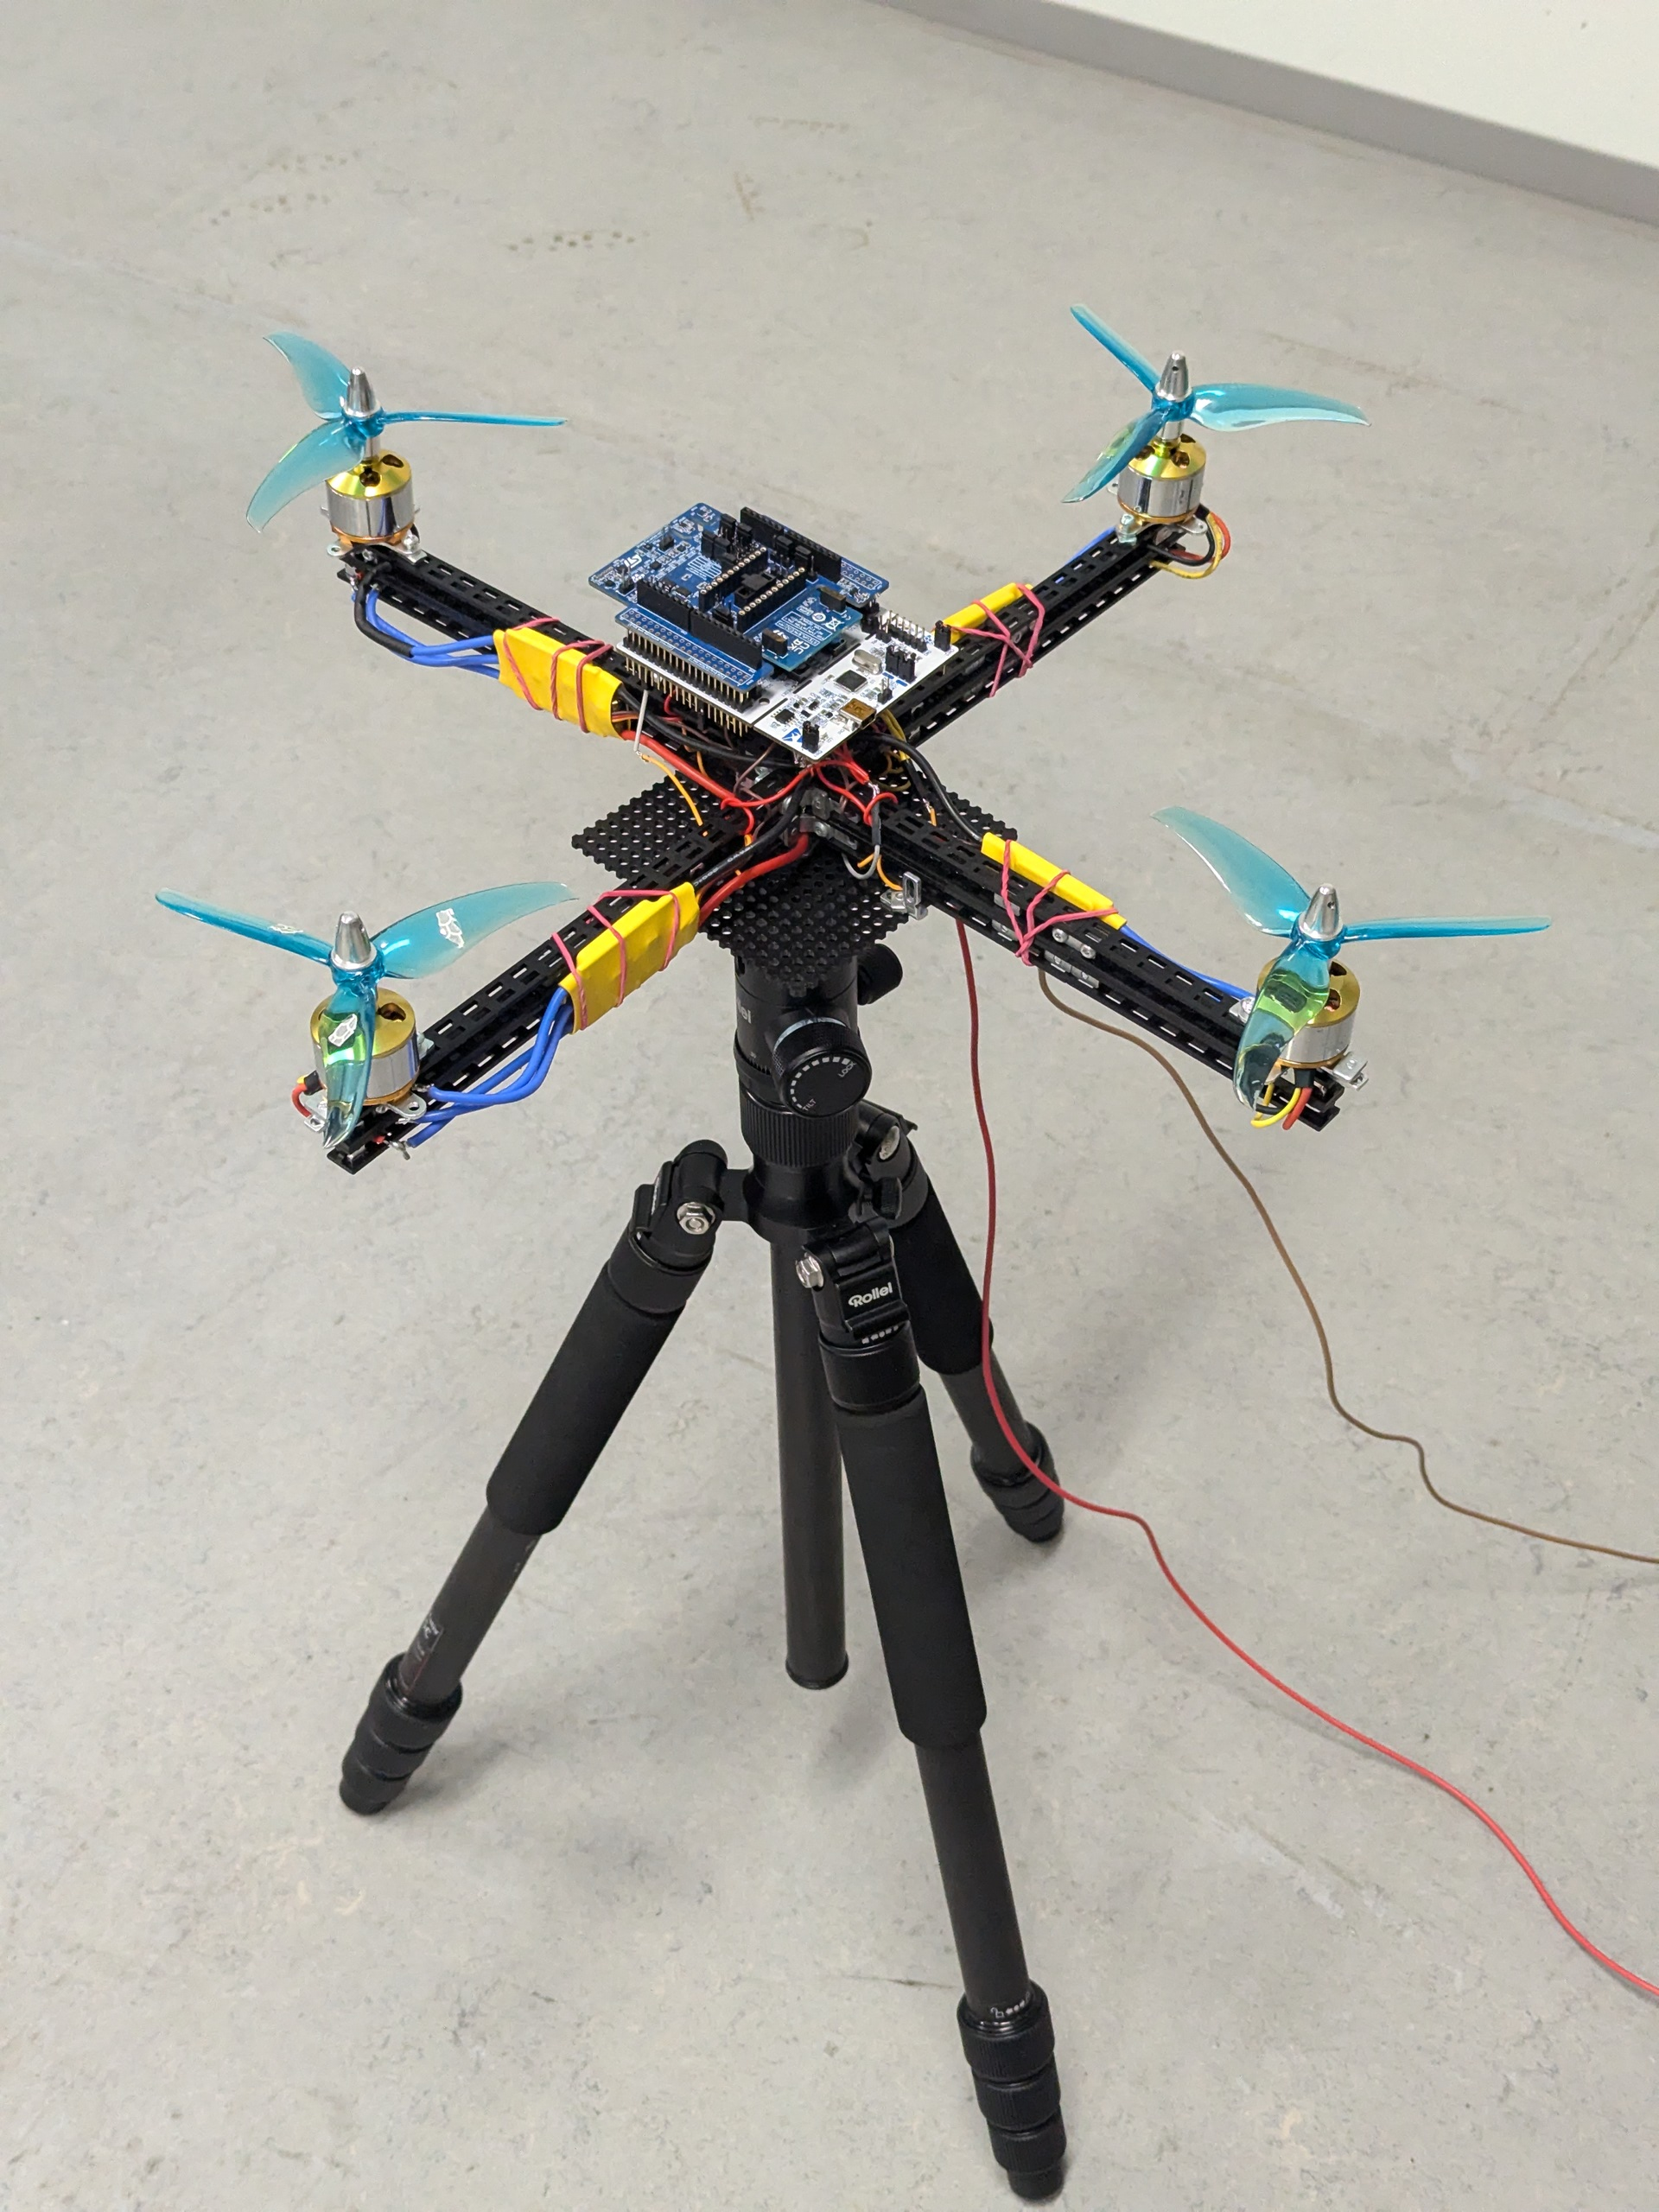
\includegraphics[scale=0.1]{../images/0070 Modell 1.jpg}{\\Prototyp 1 montiert auf einem Kamerastativ}
\end{center}


\subsection{\label{testbench:testbench}Produktion der Testbench}
Die Testbench umfasst, ein Sollwertinterface, die Visualisierung des Quadcopterzustands mittels Flask und ThreeJS sowie das Stativ, auf welchem der Quadcopter befestigt wird, mit Leistung aus einer Spannungsquelle versorgt wird und dessen Signale mit einem Oszilloskop analysiert und aufgezeichnet werden. Das Joystick-Sollwertinterface sampelt den Zustand eines Joysticks mit dem Programm \textit{joystick.py} und sendet den Schubwert und die Lage an die serielle Schnittstelle des NUCLEO-F411RE Board welche aus den Daten eine Sollgeschwindigkeit für den Regler berechnet. Die Samplefrequenz ist Default auf 30Hz eingestellt. Im Gegensatz zum Sollwertinterface welches für das Training der Agenten eingesetzt wurde tangiert das Sollwertinterface nun nicht mehr nur Informationsflussteilsysteme.
Das Pythonprogramm \textit{joystick.py} nutzt die Funktionalitäten der Bibliothek Pygame, wodurch viele verschiedene Joysticks unterstützt werden.\\
\begin{center}
	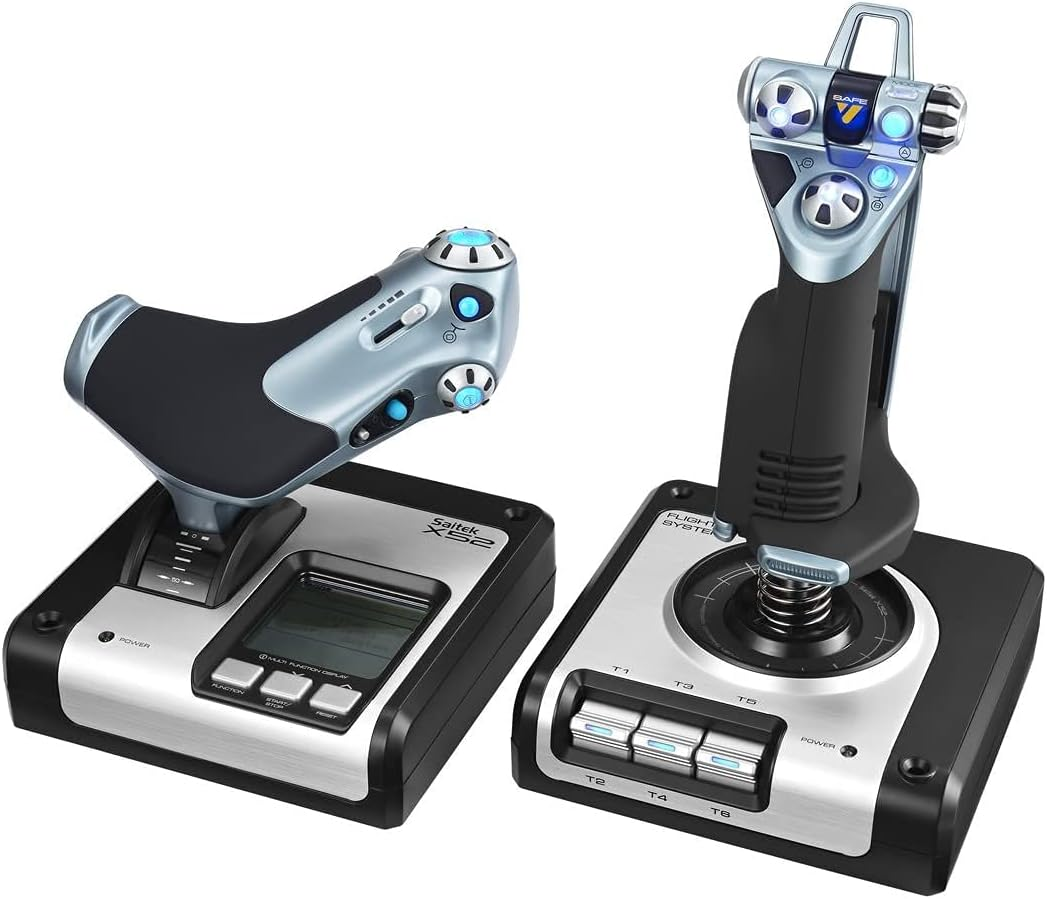
\includegraphics[scale=0.125]{../images/0063 Joystick.jpg
	}{\\Eingesetzter Joystick Saitek X52 \ref{bild:4}}
\end{center}
Der Joystickzustand wird, wenn sich ein Wert ändert, an \textit{quadseriell.py} weitergeleitet und mit der Bibliothek \textit{pyserial} an den Quadcopter gesendet. Der UART-Callback wurde erweitert, um die Joystickbefehle zu prozessieren. Die Befehle für die Nick-, Rollrichtung und den Schub werden auf Intervalle modelliert in welchen alle Werte dreistellig sind. Dadurch wird die Eindeutigkeit der Stellen sichergestellt. Im Callback werden die Werte extrahiert, zurück moduliert und in globale Variablen geschrieben. Am Joystick kann mit einem Radregler welcher visuelles Feedback gibt ein Modus selektiert werden.
\begin{center}
	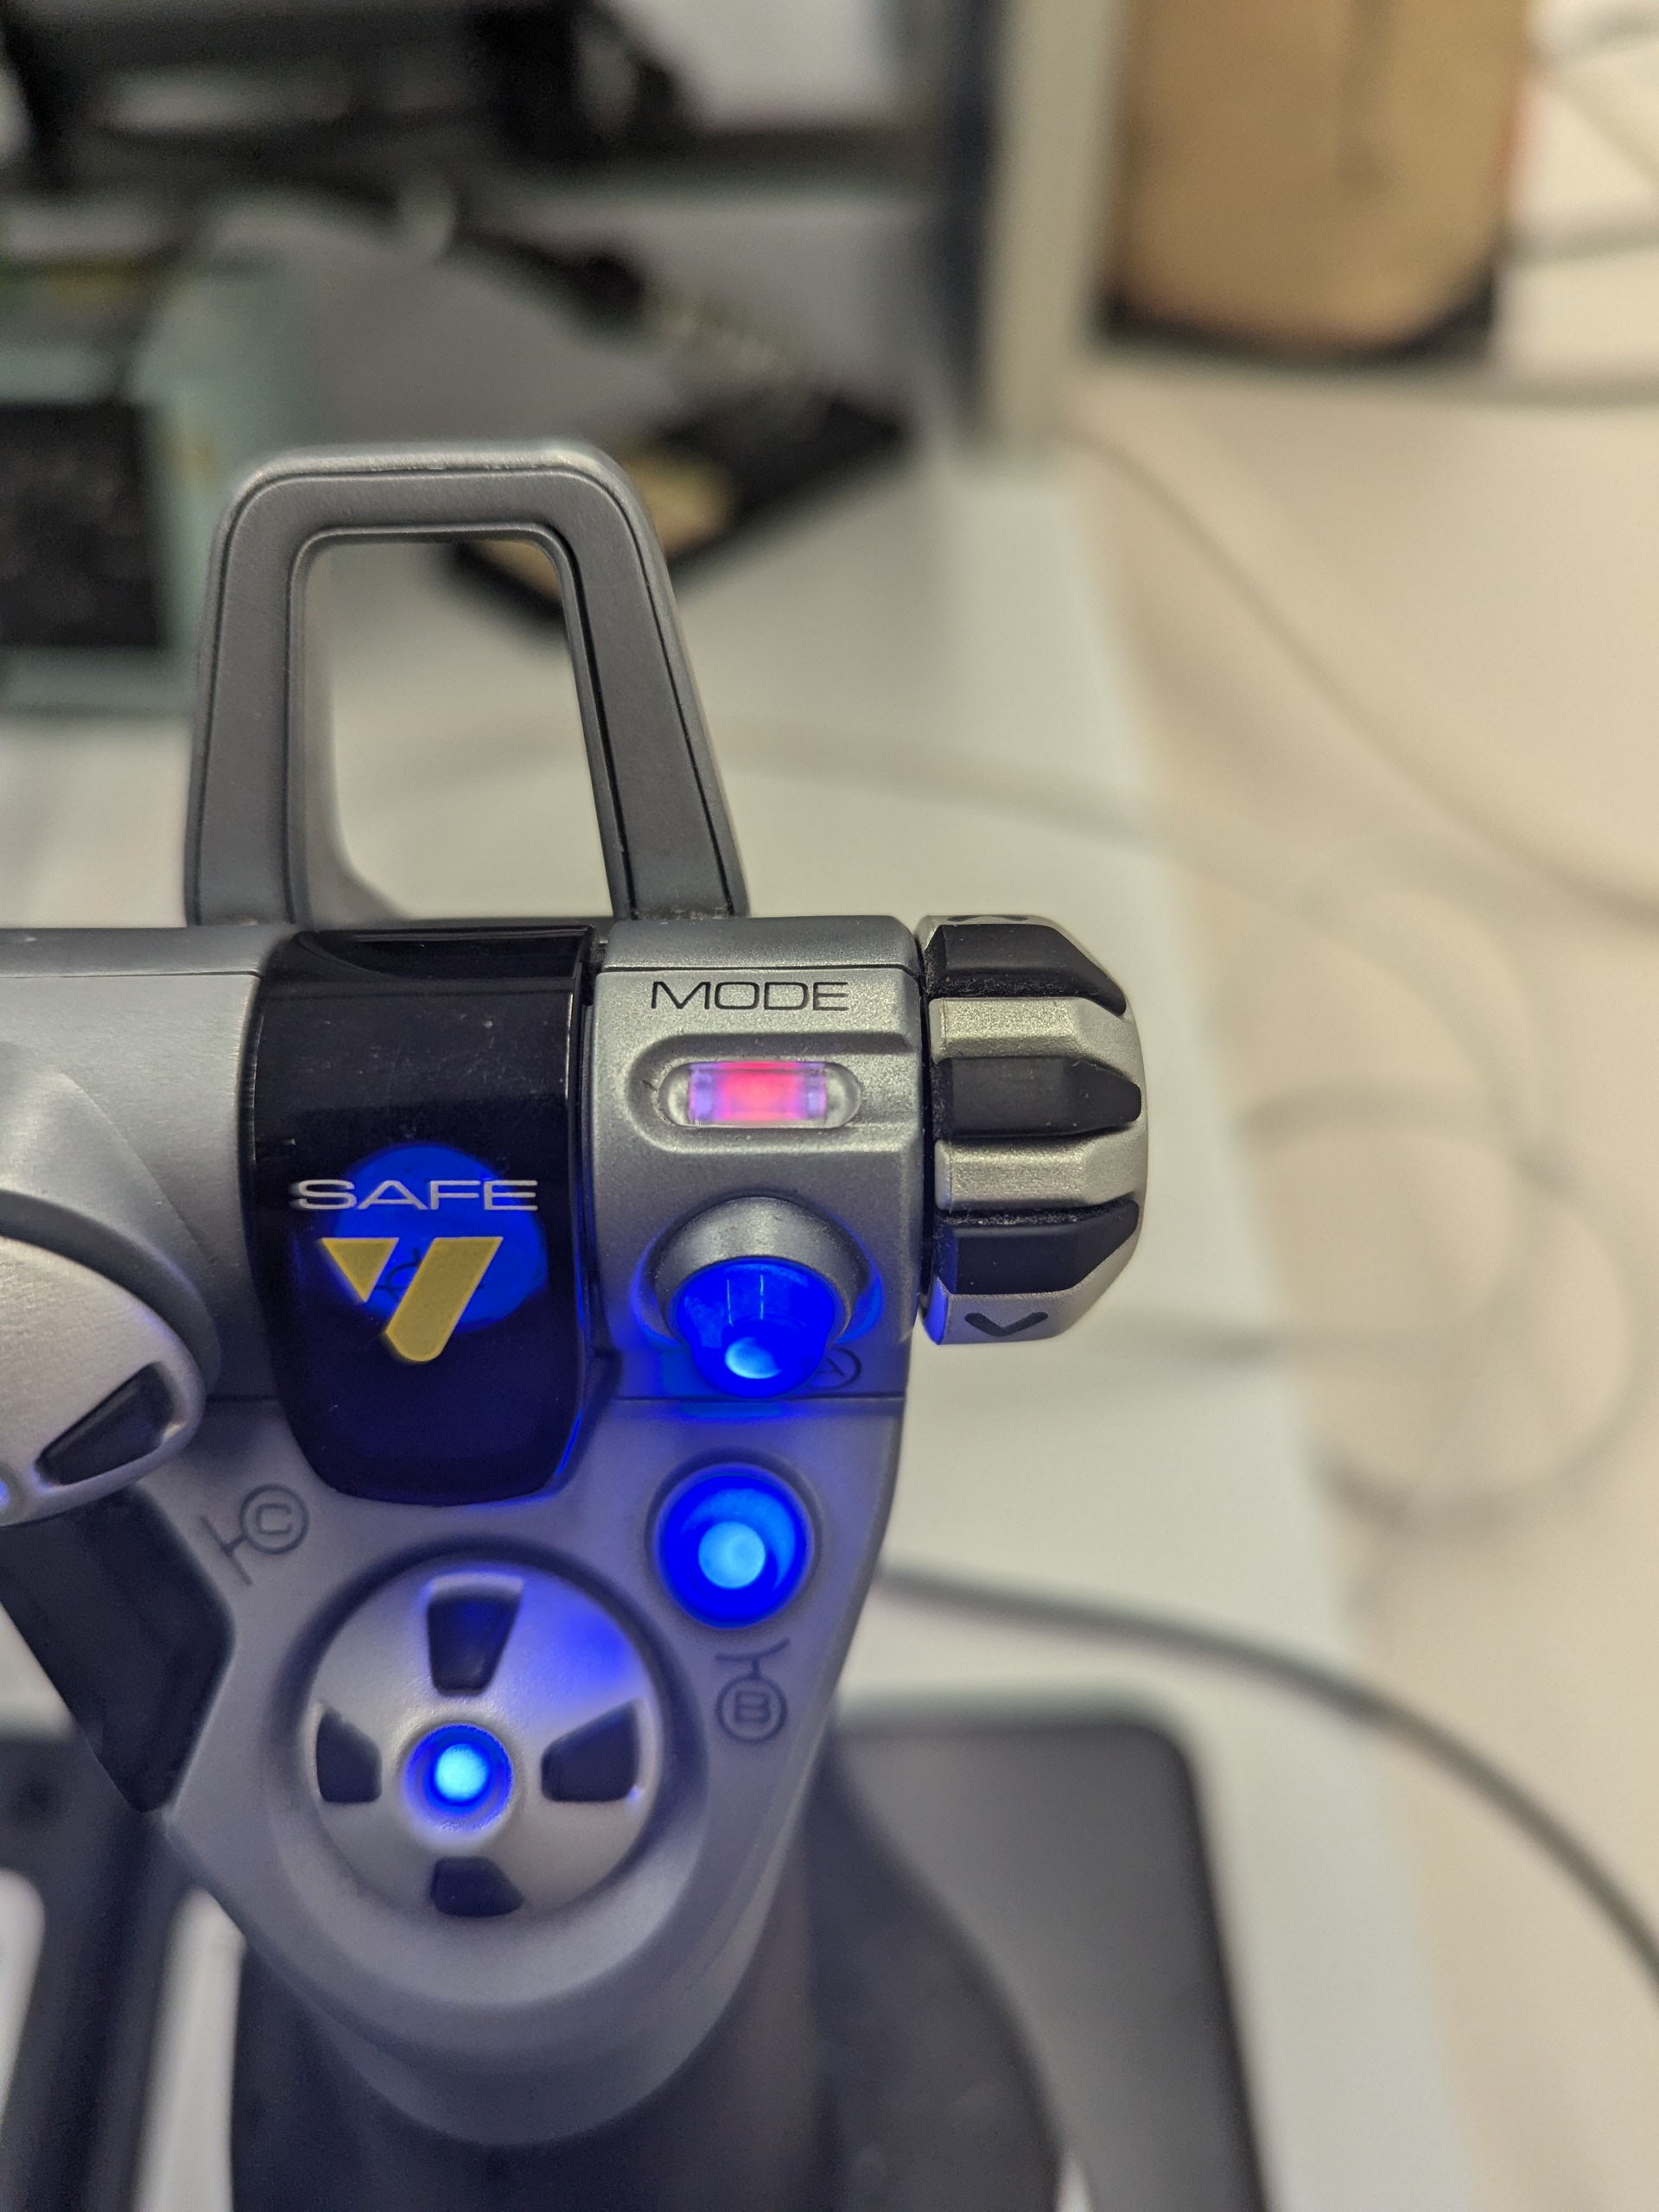
\includegraphics[scale=0.08]{../images/0088 Joystick Mode.jpg}{\\Modus 1 am Joystick ist eingestellt und die LED leuchtet leicht rot.}
\end{center}
Im Modus 0 haben Änderungen am Joystick keinen Effekt auf den Quadcopter. Im Modus 1 entspricht der Joystickschubprozentsatz direkt dem Duty-Cycle wodurch die Drehzahlregler und BLDC-Motoren getestet und programmiert werden können. Der Regler wird aktiv, wenn der Nutzer in Modus 2 wechselt.
\begin{center} 
\begin{tikzpicture}[font=\sffamily,every label/.append
style={font=\small\sffamily,align=center}]

\node[doc, fill=white] (Quadcontroller) {quadcontroller.c\\  \begin{lstlisting}[language=C, basicstyle=\fontsize{8}{10}\selectfont]
...
void USART_CharReception_Callback(void)
{
	/* Auslesen des Zeichens. */
	__IO uint32_t received_char = LL_USART_ReceiveData8(USARTx_INSTANCE);

	if (received_char == '\r') {
		rx_index = 0;
		joystick_schub = (
			100 * ((rx_buffer[0] - '0') - 1) + 
			10 * (rx_buffer[1] - '0') + 
			(rx_buffer[2] - '0')
		);
		if (joystick_schub < 5.0f) {
			regleran = 0;
		} else {
			regleran = 1;
		}
		joystick_nicken = (
			100 * rx_buffer[3] + 10 * rx_buffer[4] + rx_buffer[5] - 500
		);
		joystick_rollen = (
			100 * rx_buffer[6] + 10 * rx_buffer[7] + rx_buffer[8] - 500
		);
		modus2 = rx_buffer[9];
	  	modus1 = rx_buffer[10];
	} else {
		rx_buffer[rx_index] = received_char - '0';
		rx_index += 1;
	}
}
...
\end{lstlisting}
};
\end{tikzpicture}
\end{center}
Die Stromversorgung des Quadcopters wird auf der Testbench mit Kabel sichergestellt welche an ein Netzteil oder einen Lithium-Polymer-Akkumulator geklemmt werden können.\\
Im Modellbaubereich werden Akkus standardisiert nach der Anzahl der in Serie geschalteten Standardzellen. Eine Standardzelle hat 3.7V und wird als S1 bezeichnet. Für den Quadcopter wurde sowohl mit 7.4V als auch mit 11.1V gearbeitet, also mit S2 und S3 Akkus. Wichtig ist einen Kondensator parallel zur Spannungsquelle zu schalten um die Gleichspannung zu stabilieren und auf diese Weise die Elektronik vor Spannungsprüngen und Störrauschen zu 
schützen.
\begin{center}
	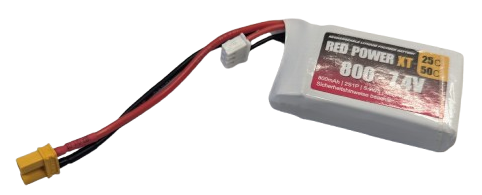
\includegraphics[scale=0.42]{../images/0082 Akku.png}{\\\label{Akku}S2 Akkumulator welcher als Alternativ zu einem Netzteil verwendet werden kann}
\end{center}
Die Montierung des Quadcopters auf einem Kamerastativ war nützlich. Mit leichten Modifikationen und Bauteilen aus dem \textit{Totem} Bausatz konnte der Quadcopter sicher fixiert werden auch ohne festgeschraubt werden zu müssen.
\begin{center}
	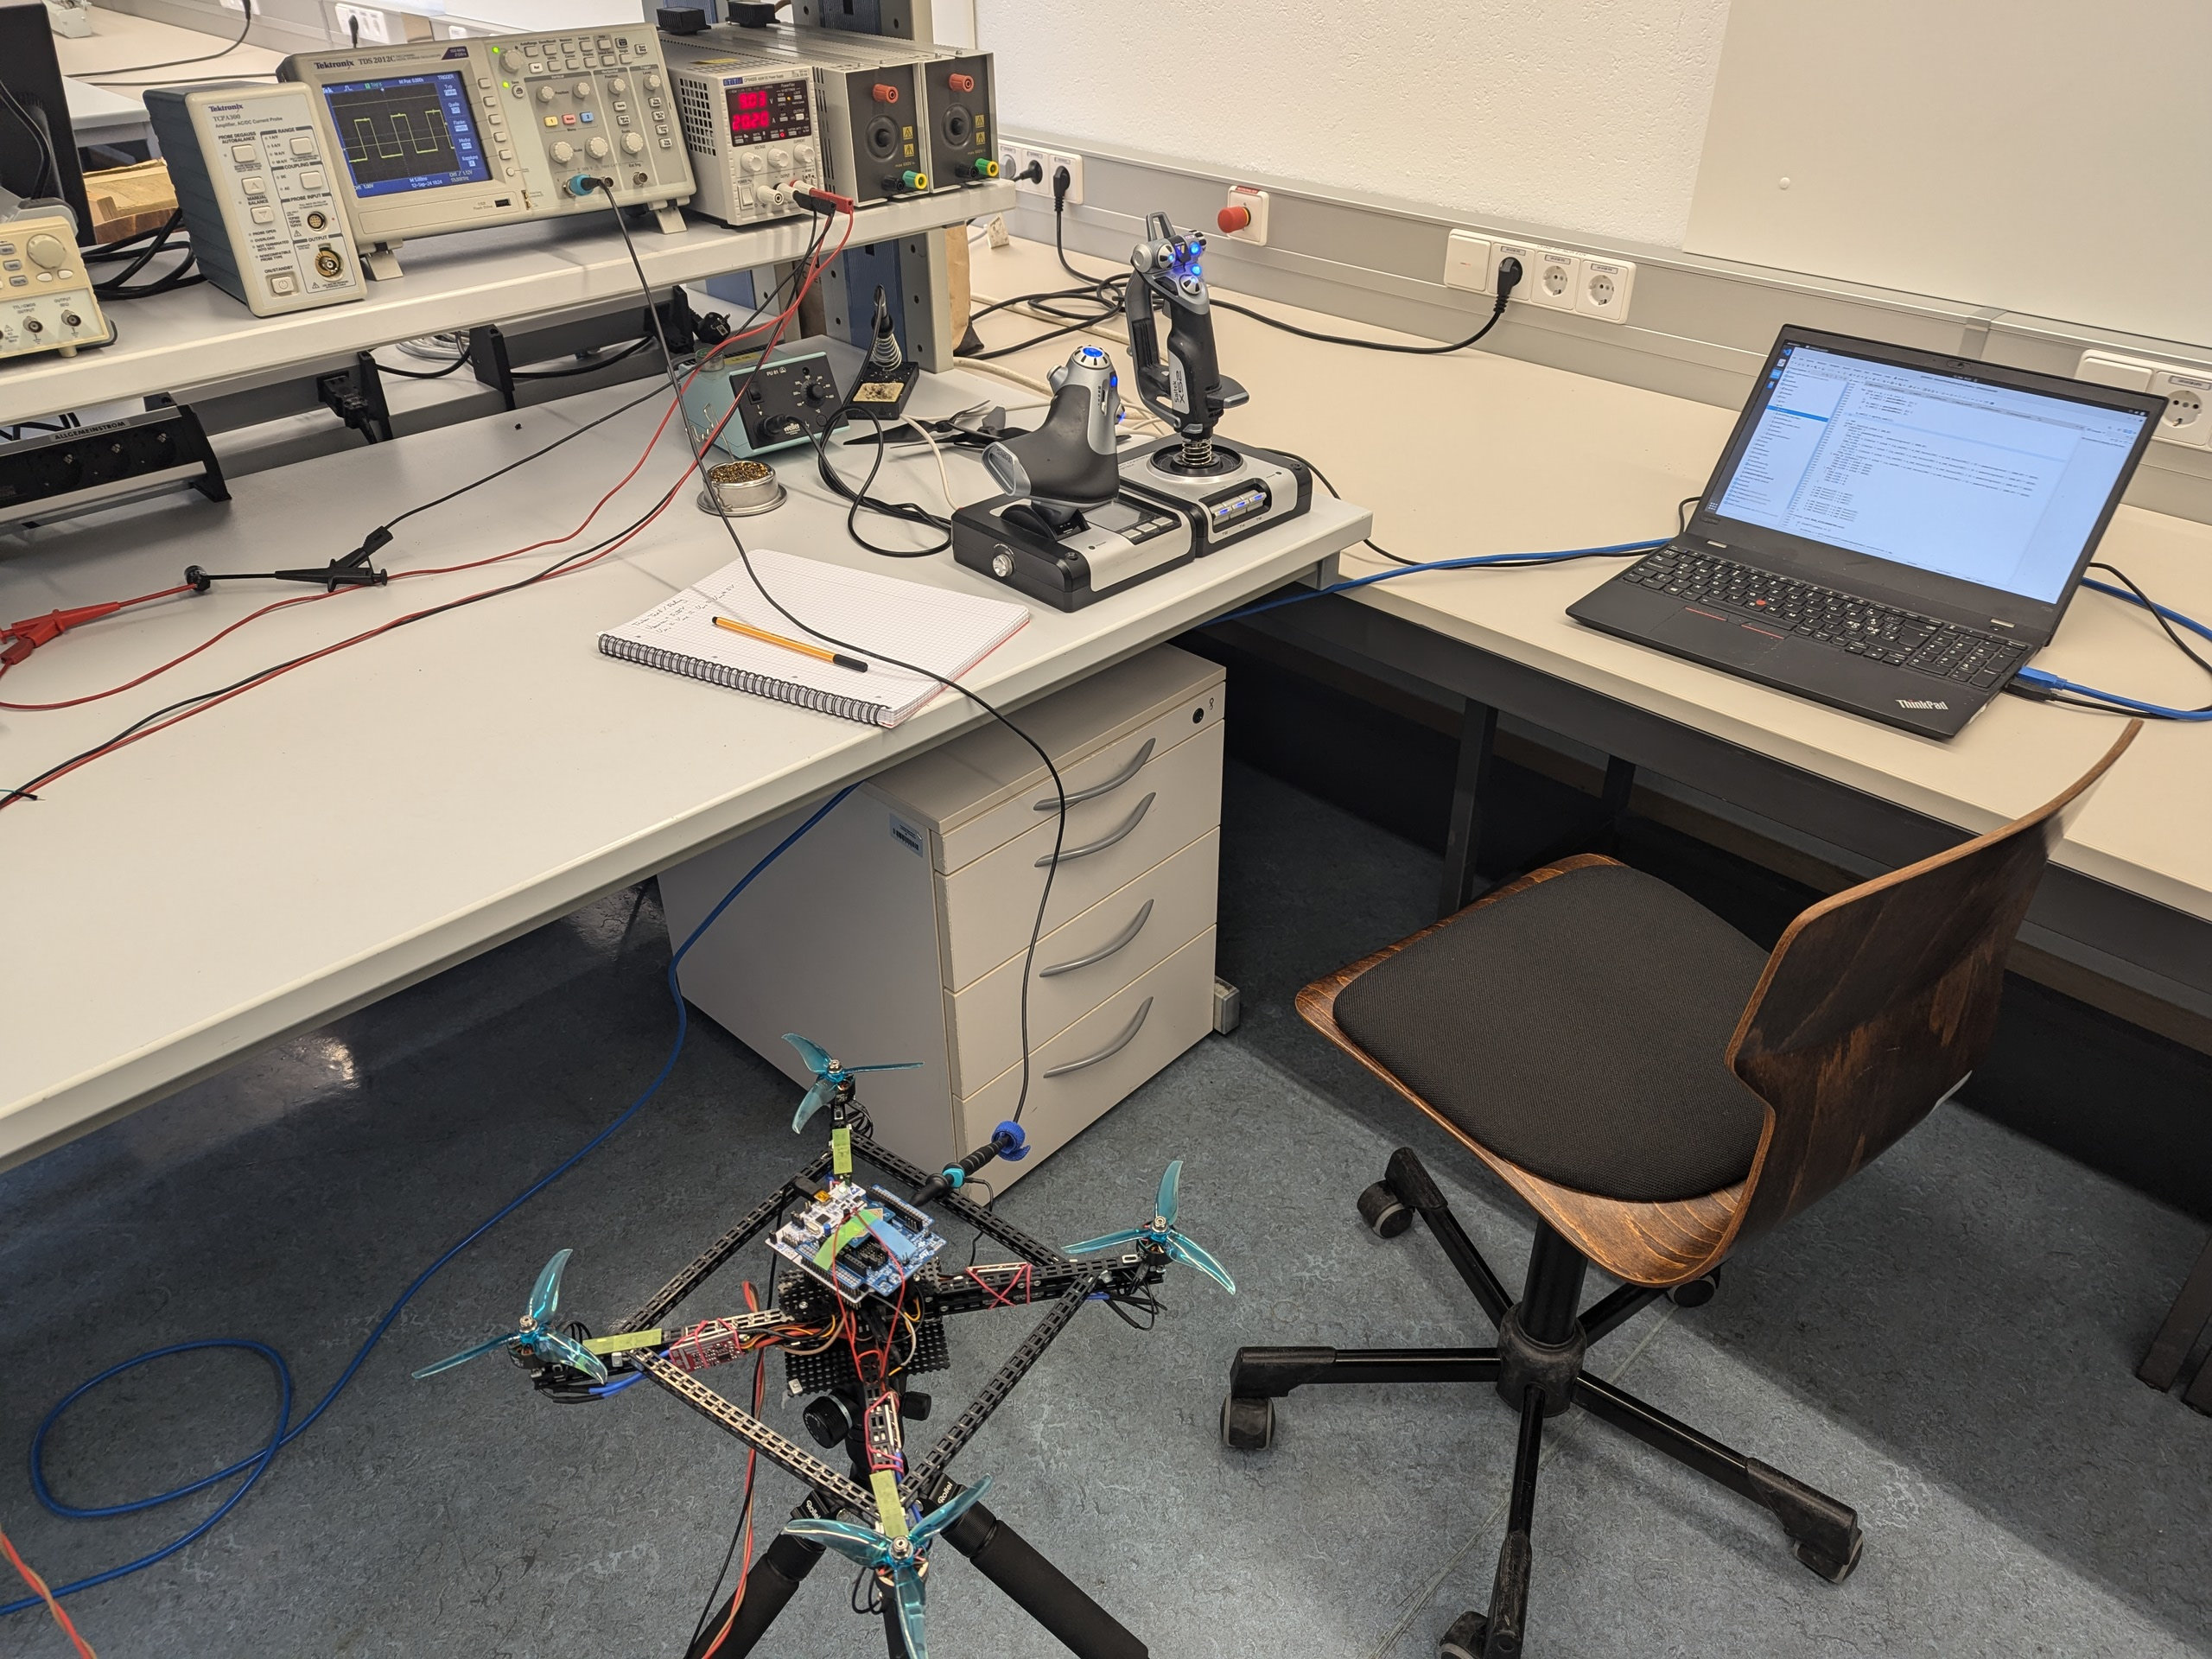
\includegraphics[scale=0.18]{../images/0087 Testbench.jpg}{\\Prototyp 2 montiert auf dem Stativ mit dem Testsetup im Hintergrund}
\end{center}

\subsection{Adaption}
Der Adaptionsteilprozess enthält alle Arbeitsschritte die anfallen, wenn ein neues Teilziel definiert wird oder ein Ziel abgeändert wird. Beispielsweise wurden neue BLDC-Motoren beschafft da die ursprünglich vorgesehenen nicht die gewünschte Drehzahl erreichten. Der Beschaffungsprozess musste also adaptiert werden. Der Adaptionsteilprozess bezieht sich immer auf mindestens einen anderen Teilprozess.\\
Auch Teil der Adaptionsphase waren erste vorsichtige Flugtests welche zur Evaluation und Optimierung des Reglers ausgewertet wurden.
\begin{center}
	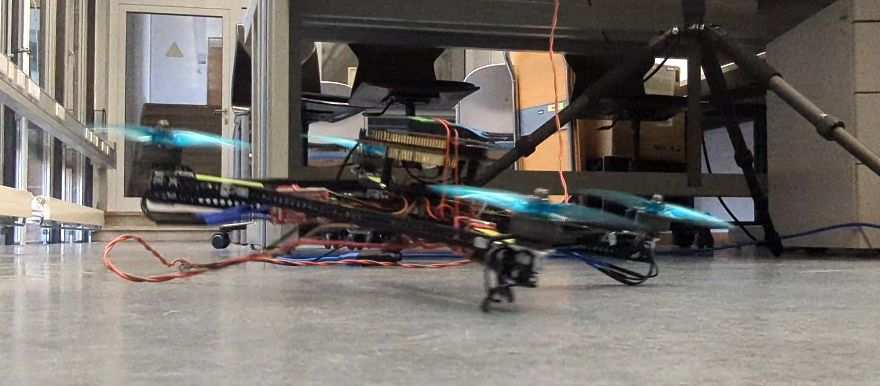
\includegraphics[scale=0.4]{../images/0073 Flugtest.png}{\\Flugtest mit PID-Regler und Joysticksollwertinterface mit Schräglage gleich nach dem Start.}
\end{center}
\begin{center}
	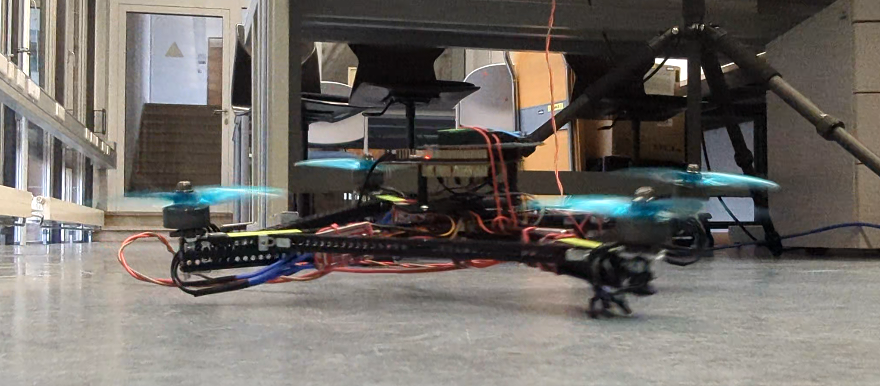
\includegraphics[scale=0.4]{../images/0074 Flugtest.png}{\\Weiterer Flugtest mit PID-Regler und Joysticksollwertinterface bei dem der Quadcopter sich auch schnell zur Seite neigt und instabil wird. Auch ein Gegensteuern am Joystick zeigt kaum Wirkung.}
\end{center}
\begin{center}
	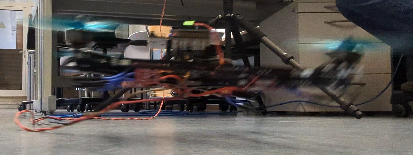
\includegraphics[scale=0.85]{../images/0075 Flugtest.png}{\\Der Quadcopter gewinnt an Höhe doch wird kurz darauf instabil.}
\end{center}
Im aktuellen Zustand geht es bei den Flugtests vor allem darum, den Regler zu debuggen und geeignete PID- und Sensorfusionsparameter zu testen. Die ersten Fehlversuche des Quadcopters wurden noch nicht ausreichend untersucht um abschließend festhalten zu können, warum der Quadcopter schnell instabil wird. Sehr wahrscheinlich ist, dass sich einer der Drehzahlregler kurz nach dem Start ausschaltet. Hinweise dafür ist ein Ton der wenige Sekunden nach dem Abheben zu hören ist und die Tatsache das einer der BLDC-Motoren in einem anderen Duty-Cycle Bereich aktiv wird beim Hochfahren. Möglich ist das der Drehzahlregler defekt oder falsch programmiert ist. Unwahrscheinlicher ist ein Fehler im Regler selbst da dieser in Test die richtigen Motorbefehle demonstrierte und das statische Verhalten der BLDC-Motoren einen korrekten Eindruck macht. Auch nicht auszuschließen ist, dass der Kalman-Filter durch die Eigenschwingungen des Quadcopters gestört wird. Maßnahmen zur Schwingungsminimierung wurden getroffen mit einem verstärkten Rahmen und gefederter Lagerung des Mikrocontrollers sind aber potenziell unzulänglich.\\
Im letzten Implementierung- beziehungsweise Adaptionsschritt wurden alle Software-, Hardwarekomponenten und die Dokumentation auf das wesentliche reduziert, getestet, validiert und geprüft.
Ziel dabei war das Gesamtsystem in einen Zustand zu bringen der zukünftigen Arbeiten so einfach wie möglich macht. Das Problem dabei ist, dass zukünftige Anforderung unbekannt sind. Nichtsdestotrotz lohnt es sich immer auf Nutzerfreundlichkeit zu achten.

\section{Zusammenfasssung}
Entwickelt wurde ein System welches sich aus Impuls-, Energie- und Informationsflussteilsystemen zusammensetzt und eignet zur Simulation, Optimierung und Entwicklung von Quadcopterreglern. Das Gesamtsystem kann auch von Nutzern mit geringer Programmiererfahrung bedient werden.\\
Die Entwicklung von serienreifen Reglern auf Basis von der Software ist noch in ihren Anfängen. So wurden diverse Modelle antrainiert welche teilweise erste Anzeichen von Qualität zeigen. Weiteres Hyperparametertuning ist notwendig um die gelernten Regler auf ein Markttaugliches Niveau zu bringen. Auch sind die Regler für sich genommen unspektakulär. Die Integration von weitere Funktionen wie Trajektorien-Folgeregelung oder Multi-Agenten-Simulationen können zukünftige Schritte sein, um den Nutzen des Gesamtsystems weiter zu steigern.\\
Die Entwicklung des physikalisch Quadcopters ist in den letzten Zügen, noch zu optimieren beziehungsweise zu debuggen sind die Drehzahlregler sowie die Parametrisierung der Sensordatenfusion. Die Integration von einem Regler welcher mit gelernten Parameter oder direkt mit einem Ende-zu-Ende-Modell arbeiten ist auch schon in Aussicht.

\section{Referenzen}
\subsection{Literatur}
\begin{enumerate}[label=\textbf{[\arabic*]}]
	\item \label{link:Regelungstechnik1}Günter Ludyk, Theoretische Regelungstechnik 1, Springer Verlag, 1995
	\item \label{link:Regelungstechnik2}Günter Ludyk, Theoretische Regelungstechnik 2, Springer Verlag, 1995
	\item \label{link:MaschinellesLernen}Jörg Frochte, Maschinelles Lernen Grundlagen und Algorithmen in Python, Carl Hanser Verlag, 04.02.2024
	\item \label{link:DeepReinforcementLearning}Alexander Zai; Brandon Brown, Einstieg in Deep Reinforcement Learning, Carl Hanser Verlag, 2020 
	\item \label{link:Python}Michael Weigend, Python 3 Lernen und professionell anwenden 8. erweiterte Auflage, mitp, 2018 
	\item \label{link:Betriebswirtschaftslehre}Günter Wöhe; Ulrich Döring; Gerrit Brösel, Einführung in die Allgemeine Betriebswirtschaftslehre 28. Auflage, Vahlen, 2024
	\item \label{link:ReinforcementLearningQuadcopter}Fang-I Hsiao; Cheng-Min Chiang; Alvin Hou, Reinforcement Learning Based Quadcopter
	Controller, Stanford, 2019
	\item \label{link:Modelle}Jeffrey Koperski, Models, https://iep.utm.edu/models/, Internet Encyclopedia of Philosophy, abgerufen am 26.08.2024
	\item \label{link:LocalTangent}Local tangent plane coordinates, https://en.wikipedia.org/wiki/Local\_tangent\_\\plane\_coordinates, Wikipedia, abgerufen am 08.09.24
	\item \label{link:Flask}Flask Dokumentation, https://flask.palletsprojects.com/en/3.0.x/, Flask, abgerufen am 24.08.24
	\item \label{link:PWM}STM32 PWM Example - Timer PWM Mode Tutorial, https://deepbluembedded.com/stm32-pwm-example-timer-pwm-mode-tutorial/, abgerufen am 22.08.2024
	\item \label{link:Eulerwinkel}Eulerwinkel, http://groolfs.de/Verschiedenespdf/EulerWinkel.pdf, Eulerwinkel, abgerufen am 15.08.2024
	\item \label{link:Zephyr}Zephyr, https://zephyrproject.org/, Zephyr, abgerufen am 14.08.2024
	\item \label{link:PPOSpinningUp}Proximal Policy Optimization, https://spinningup.openai.com/en/latest/algorithms/\\ppo.html, OpenAI, abgerufen am 18.08.2024
	\item \label{link:Sensorfusion}Sensorfusion, https://www.iis.fraunhofer.de/de/ff/lv/dataanalytics/sensorfusion.html,\\
	Fraunhofer IIS, abgerufen am 08.09.2024
	\item \label{link:Quaternion}Rotation Quaternions and how to Use Them, https://danceswithcode.net/engineeringnotes/\\
	quaternions/quaternions.html, abgerufen am 08.09.2024
	\item \label{link:MotorControl}Motor control, http://stickyfish.dk/Motor Control.html, Raspberry Fly, abgerufen am 08.09.2024
	\item \label{link:DeepLearningStateEstimation}Deep-Learning-Based-State-Estimation, zshicode, https://
	github.com/zshicode/\\Deep-Learning-Based-State-Estimation, abgerufen am 08.09.2024
	\item \label{link:A2217}A2217, https://www.suppomodel.com/motor/A2217.html, Suppo Model, abgerufen am 07.09.2024
	\item \label{link:Kane}Equations of Motion for robotic manipulators using the Kane Method,\\
	https://www.youtube.com/watch?v=QwWiY13Ptk0, abgerufen am 16.08.2024
	\item \label{link:SimCon}John Bobzwik, SimCon, Quadcopter\_SimCon, https://github.com/bobzwik/Quadcopter, abgerufen am 25.08.2024
	\item \label{link:STM32CubeBSP} UM2298 STM32Cube BSP drivers development guidelines, STMicroelectronics, 2019
	\item \label{link:31} Why do we use the log in gradient-based reinforcement algorithms?,\\
	https://cs.stackexchange.com/questions/70518/why-do-we-use-the-log-in-gradient-based-reinforcement-algorithms, StackExchange, abgerufen am 08.09.2024
	\item \label{link:32} John S; Filip W, Prafulla D; Alec R; Oleg K, Proximal Policy Optimization Algorithms, OpenAI, 2017
	\item \label{link:33} STM32F411xC/E advanced Arm® -based 32-bit MCUs, STMicroelectronics, 2018
	\item \label{link:34} Getting started with the X-NUCLEO-IKS4A1 motion MEMS and environmental sensor expansion board for STM32 Nucleo, STMicroelectronics, 2024
	\item \label{link:Treiberdatenblatt}ESC Datenblatt, 30A BLDC ESC, abgerufen am 10.09.2024 
	\item \label{link:ETH}Brescianini Dario; Hehn Markus; D'Andrea Raffaello, Nonlinear Quadrocopter Attitude Control, ETH Zürich, abgerufen am 10.09.2013 
	\item \label{link:MPC} Model Predictive Control for Quadrotors with extension to Perception-Aware MPC, https://github.com/uzh-rpg/rpg\_mpc, Robotics and Perception Group, abgerufen am 12.09.24
	\item \label{link:LogPPO} Why do we use the log in gradient-based reinforcement algorithms?,\\ https://cs.stackexchange.com/questions/70518/why-do-we-use-the-log-in-gradient-based-reinforcement-algorithms, StackExchange, abgerufen am 12.09.24
	\item \label{link:PPOBeginner}View ericyangyu's full-sized avatar Eric Yu, https://github.com/ericyangyu/PPO-for-Beginners, Github, abgerufen am 12.09.24
	\item \label{link:MotionFX}Andrea Vitali, MotionFX orientation estimation DT0075, STMicroelectronics, 2017
	\item \label{X-CUBE-MEMS1} UM2220 Getting started with MotionFX sensor fusion library in X-CUBE-MEMS1
	expansion for STM32Cube, STMicroelectronics, 2021
\end{enumerate}

\subsection{Bilderverzeichnis}
\begin{enumerate}[label=\textbf{[\arabic*]}]
	\item \label{bild:1} http://groolfs.de/Verschiedenespdf/EulerWinkel.pdf, abgerufen am 22.08.2024
	\item \label{bild:2} https://huggingface.co/learn/deep-rl-course/unit1/exp-exp-tradeoff?fw=pt, Huggingface, abgerufen am 31.08.2024
	\item \label{bild:3} https://threejs.org/examples/, abgerufen am 13.08.24
	\item \label{bild:4} https://www.amazon.co.uk/Logitech-Saitek-Flight-Control-System/dp/B01M9EWQ2W, abgerufen am 05.09.24
	\item \label{bild:Pinout} IOT-Jungle, https://www.iot-jungle.com/boutique/cpu-boards-uk/nucleo-uk/\\nucleo-f411re/, abgerufen am 11.09.24
\end{enumerate}

\subsection{Repository}
Alle Teile dieser Arbeit können in einem öffentlichen Repository gefunden werden. 
\begin{align*}
	\text{https://codeberg.org/TimStraube/Quadstar/}
\end{align*}

\end{document}
